\documentclass[twoside]{book}

% Packages required by doxygen
\usepackage{calc}
\usepackage{doxygen}
\usepackage{graphicx}
\usepackage[utf8]{inputenc}
\usepackage{makeidx}
\usepackage{multicol}
\usepackage{multirow}
\usepackage{textcomp}
\usepackage[table]{xcolor}

% Font selection
\usepackage[T1]{fontenc}
\usepackage{mathptmx}
\usepackage[scaled=.90]{helvet}
\usepackage{courier}
\usepackage{amssymb}
\usepackage{sectsty}
\renewcommand{\familydefault}{\sfdefault}
\allsectionsfont{%
  \fontseries{bc}\selectfont%
  \color{darkgray}%
}
\renewcommand{\DoxyLabelFont}{%
  \fontseries{bc}\selectfont%
  \color{darkgray}%
}

% Page & text layout
\usepackage{geometry}
\geometry{%
  a4paper,%
  top=2.5cm,%
  bottom=2.5cm,%
  left=2.5cm,%
  right=2.5cm%
}
\tolerance=750
\hfuzz=15pt
\hbadness=750
\setlength{\emergencystretch}{15pt}
\setlength{\parindent}{0cm}
\setlength{\parskip}{0.2cm}
\makeatletter
\renewcommand{\paragraph}{%
  \@startsection{paragraph}{4}{0ex}{-1.0ex}{1.0ex}{%
    \normalfont\normalsize\bfseries\SS@parafont%
  }%
}
\renewcommand{\subparagraph}{%
  \@startsection{subparagraph}{5}{0ex}{-1.0ex}{1.0ex}{%
    \normalfont\normalsize\bfseries\SS@subparafont%
  }%
}
\makeatother

% Headers & footers
\usepackage{fancyhdr}
\pagestyle{fancyplain}
\fancyhead[LE]{\fancyplain{}{\bfseries\thepage}}
\fancyhead[CE]{\fancyplain{}{}}
\fancyhead[RE]{\fancyplain{}{\bfseries\leftmark}}
\fancyhead[LO]{\fancyplain{}{\bfseries\rightmark}}
\fancyhead[CO]{\fancyplain{}{}}
\fancyhead[RO]{\fancyplain{}{\bfseries\thepage}}
\fancyfoot[LE]{\fancyplain{}{}}
\fancyfoot[CE]{\fancyplain{}{}}
\fancyfoot[RE]{\fancyplain{}{\bfseries\scriptsize Generated on Sat Sep 14 2013 15:16:06 for Burngine 3D OpenGL-Engine by Doxygen }}
\fancyfoot[LO]{\fancyplain{}{\bfseries\scriptsize Generated on Sat Sep 14 2013 15:16:06 for Burngine 3D OpenGL-Engine by Doxygen }}
\fancyfoot[CO]{\fancyplain{}{}}
\fancyfoot[RO]{\fancyplain{}{}}
\renewcommand{\footrulewidth}{0.4pt}
\renewcommand{\chaptermark}[1]{%
  \markboth{#1}{}%
}
\renewcommand{\sectionmark}[1]{%
  \markright{\thesection\ #1}%
}

% Indices & bibliography
\usepackage{natbib}
\usepackage[titles]{tocloft}
\setcounter{tocdepth}{3}
\setcounter{secnumdepth}{5}
\makeindex

% Hyperlinks (required, but should be loaded last)
\usepackage{ifpdf}
\ifpdf
  \usepackage[pdftex,pagebackref=true]{hyperref}
\else
  \usepackage[ps2pdf,pagebackref=true]{hyperref}
\fi
\hypersetup{%
  colorlinks=true,%
  linkcolor=blue,%
  citecolor=blue,%
  unicode%
}

% Custom commands
\newcommand{\clearemptydoublepage}{%
  \newpage{\pagestyle{empty}\cleardoublepage}%
}


%===== C O N T E N T S =====

\begin{document}

% Titlepage & ToC
\hypersetup{pageanchor=false}
\pagenumbering{roman}
\begin{titlepage}
\vspace*{7cm}
\begin{center}%
{\Large Burngine 3\-D Open\-G\-L-\/\-Engine \\[1ex]\large Development }\\
\vspace*{1cm}
{\large Generated by Doxygen 1.8.4}\\
\vspace*{0.5cm}
{\small Sat Sep 14 2013 15:16:06}\\
\end{center}
\end{titlepage}
\clearemptydoublepage
\tableofcontents
\clearemptydoublepage
\pagenumbering{arabic}
\hypersetup{pageanchor=true}

%--- Begin generated contents ---
\chapter{Namespace Index}
\section{Namespace List}
Here is a list of all namespaces with brief descriptions\-:\begin{DoxyCompactList}
\item\contentsline{section}{\hyperlink{namespaceburn}{burn} \\*$<$-\/ G\-L\-F\-W }{\pageref{namespaceburn}}{}
\end{DoxyCompactList}

\chapter{Hierarchical Index}
\section{Class Hierarchy}
This inheritance list is sorted roughly, but not completely, alphabetically\-:\begin{DoxyCompactList}
\item \contentsline{section}{burn\-:\-:Base\-Texture}{\pageref{classburn_1_1_base_texture}}{}
\begin{DoxyCompactList}
\item \contentsline{section}{burn\-:\-:Cube\-Map}{\pageref{classburn_1_1_cube_map}}{}
\item \contentsline{section}{burn\-:\-:Render\-Texture}{\pageref{classburn_1_1_render_texture}}{}
\item \contentsline{section}{burn\-:\-:Shadow\-Cube\-Map}{\pageref{classburn_1_1_shadow_cube_map}}{}
\item \contentsline{section}{burn\-:\-:Shadow\-Map}{\pageref{classburn_1_1_shadow_map}}{}
\item \contentsline{section}{burn\-:\-:Texture}{\pageref{classburn_1_1_texture}}{}
\end{DoxyCompactList}
\item \contentsline{section}{burn\-:\-:Burngine\-Shaders}{\pageref{structburn_1_1_burngine_shaders}}{}
\item \contentsline{section}{burn\-:\-:Character}{\pageref{classburn_1_1_character}}{}
\item \contentsline{section}{burn\-:\-:Clock}{\pageref{classburn_1_1_clock}}{}
\item \contentsline{section}{burn\-:\-:Font}{\pageref{classburn_1_1_font}}{}
\item \contentsline{section}{burn\-:\-:G\-Buffer}{\pageref{classburn_1_1_g_buffer}}{}
\item \contentsline{section}{burn\-:\-:Gui}{\pageref{classburn_1_1_gui}}{}
\item \contentsline{section}{burn\-:\-:Gui\-Node}{\pageref{classburn_1_1_gui_node}}{}
\begin{DoxyCompactList}
\item \contentsline{section}{burn\-:\-:Rectangle\-Shape}{\pageref{classburn_1_1_rectangle_shape}}{}
\item \contentsline{section}{burn\-:\-:Text}{\pageref{classburn_1_1_text}}{}
\begin{DoxyCompactList}
\item \contentsline{section}{burn\-:\-:Label}{\pageref{classburn_1_1_label}}{}
\end{DoxyCompactList}
\end{DoxyCompactList}
\item \contentsline{section}{burn\-:\-:Keyboard}{\pageref{classburn_1_1_keyboard}}{}
\item \contentsline{section}{burn\-:\-:Material}{\pageref{classburn_1_1_material}}{}
\item \contentsline{section}{burn\-:\-:Mesh}{\pageref{classburn_1_1_mesh}}{}
\item \contentsline{section}{burn\-:\-:Model}{\pageref{classburn_1_1_model}}{}
\item \contentsline{section}{burn\-:\-:Mouse}{\pageref{classburn_1_1_mouse}}{}
\item \contentsline{section}{burn\-:\-:Open\-Gl\-Control}{\pageref{classburn_1_1_open_gl_control}}{}
\item \contentsline{section}{burn\-:\-:Rectangle$<$ T $>$}{\pageref{classburn_1_1_rectangle}}{}
\item \contentsline{section}{burn\-:\-:Reporter}{\pageref{classburn_1_1_reporter}}{}
\item \contentsline{section}{burn\-:\-:Sampler}{\pageref{classburn_1_1_sampler}}{}
\item \contentsline{section}{burn\-:\-:Scene}{\pageref{classburn_1_1_scene}}{}
\item \contentsline{section}{burn\-:\-:Open\-Gl\-Control\-:\-:Settings}{\pageref{classburn_1_1_open_gl_control_1_1_settings}}{}
\item \contentsline{section}{burn\-:\-:Shader}{\pageref{classburn_1_1_shader}}{}
\item \contentsline{section}{burn\-:\-:Sky\-Box}{\pageref{classburn_1_1_sky_box}}{}
\item \contentsline{section}{burn\-:\-:String}{\pageref{classburn_1_1_string}}{}
\item \contentsline{section}{burn\-:\-:Time}{\pageref{classburn_1_1_time}}{}
\item \contentsline{section}{burn\-:\-:Transformable}{\pageref{classburn_1_1_transformable}}{}
\begin{DoxyCompactList}
\item \contentsline{section}{burn\-:\-:Camera}{\pageref{classburn_1_1_camera}}{}
\item \contentsline{section}{burn\-:\-:Light}{\pageref{classburn_1_1_light}}{}
\begin{DoxyCompactList}
\item \contentsline{section}{burn\-:\-:Directional\-Light}{\pageref{classburn_1_1_directional_light}}{}
\begin{DoxyCompactList}
\item \contentsline{section}{burn\-:\-:Spot\-Light}{\pageref{classburn_1_1_spot_light}}{}
\end{DoxyCompactList}
\end{DoxyCompactList}
\item \contentsline{section}{burn\-:\-:Scene\-Node}{\pageref{classburn_1_1_scene_node}}{}
\begin{DoxyCompactList}
\item \contentsline{section}{burn\-:\-:Static\-Mesh\-Node}{\pageref{classburn_1_1_static_mesh_node}}{}
\end{DoxyCompactList}
\end{DoxyCompactList}
\item \contentsline{section}{burn\-:\-:Utf$<$ N $>$}{\pageref{classburn_1_1_utf}}{}
\item \contentsline{section}{burn\-:\-:Utf$<$ 16 $>$}{\pageref{classburn_1_1_utf_3_0116_01_4}}{}
\item \contentsline{section}{burn\-:\-:Utf$<$ 32 $>$}{\pageref{classburn_1_1_utf_3_0132_01_4}}{}
\item \contentsline{section}{burn\-:\-:Utf$<$ 8 $>$}{\pageref{classburn_1_1_utf_3_018_01_4}}{}
\item \contentsline{section}{burn\-:\-:Vertex}{\pageref{classburn_1_1_vertex}}{}
\item \contentsline{section}{burn\-:\-:Vertex\-Buffer\-Object}{\pageref{classburn_1_1_vertex_buffer_object}}{}
\item \contentsline{section}{burn\-:\-:Window}{\pageref{classburn_1_1_window}}{}
\item \contentsline{section}{burn\-:\-:Window\-Settings}{\pageref{classburn_1_1_window_settings}}{}
\end{DoxyCompactList}

\chapter{Class Index}
\section{Class List}
Here are the classes, structs, unions and interfaces with brief descriptions\-:\begin{DoxyCompactList}
\item\contentsline{section}{\hyperlink{classburn_1_1_base_texture}{burn\-::\-Base\-Texture} }{\pageref{classburn_1_1_base_texture}}{}
\item\contentsline{section}{\hyperlink{structburn_1_1_burngine_shaders}{burn\-::\-Burngine\-Shaders} }{\pageref{structburn_1_1_burngine_shaders}}{}
\item\contentsline{section}{\hyperlink{classburn_1_1_camera}{burn\-::\-Camera} }{\pageref{classburn_1_1_camera}}{}
\item\contentsline{section}{\hyperlink{classburn_1_1_character}{burn\-::\-Character} }{\pageref{classburn_1_1_character}}{}
\item\contentsline{section}{\hyperlink{classburn_1_1_clock}{burn\-::\-Clock} }{\pageref{classburn_1_1_clock}}{}
\item\contentsline{section}{\hyperlink{classburn_1_1_cube_map}{burn\-::\-Cube\-Map} }{\pageref{classburn_1_1_cube_map}}{}
\item\contentsline{section}{\hyperlink{classburn_1_1_directional_light}{burn\-::\-Directional\-Light} }{\pageref{classburn_1_1_directional_light}}{}
\item\contentsline{section}{\hyperlink{classburn_1_1_font}{burn\-::\-Font} }{\pageref{classburn_1_1_font}}{}
\item\contentsline{section}{\hyperlink{classburn_1_1_g_buffer}{burn\-::\-G\-Buffer} }{\pageref{classburn_1_1_g_buffer}}{}
\item\contentsline{section}{\hyperlink{classburn_1_1_gui}{burn\-::\-Gui} }{\pageref{classburn_1_1_gui}}{}
\item\contentsline{section}{\hyperlink{classburn_1_1_gui_node}{burn\-::\-Gui\-Node} }{\pageref{classburn_1_1_gui_node}}{}
\item\contentsline{section}{\hyperlink{classburn_1_1_keyboard}{burn\-::\-Keyboard} }{\pageref{classburn_1_1_keyboard}}{}
\item\contentsline{section}{\hyperlink{classburn_1_1_label}{burn\-::\-Label} }{\pageref{classburn_1_1_label}}{}
\item\contentsline{section}{\hyperlink{classburn_1_1_light}{burn\-::\-Light} }{\pageref{classburn_1_1_light}}{}
\item\contentsline{section}{\hyperlink{classburn_1_1_material}{burn\-::\-Material} }{\pageref{classburn_1_1_material}}{}
\item\contentsline{section}{\hyperlink{classburn_1_1_mesh}{burn\-::\-Mesh} }{\pageref{classburn_1_1_mesh}}{}
\item\contentsline{section}{\hyperlink{classburn_1_1_model}{burn\-::\-Model} \\*A model can load 3d models from file }{\pageref{classburn_1_1_model}}{}
\item\contentsline{section}{\hyperlink{classburn_1_1_mouse}{burn\-::\-Mouse} }{\pageref{classburn_1_1_mouse}}{}
\item\contentsline{section}{\hyperlink{classburn_1_1_open_gl_control}{burn\-::\-Open\-Gl\-Control} }{\pageref{classburn_1_1_open_gl_control}}{}
\item\contentsline{section}{\hyperlink{classburn_1_1_rectangle}{burn\-::\-Rectangle$<$ T $>$} }{\pageref{classburn_1_1_rectangle}}{}
\item\contentsline{section}{\hyperlink{classburn_1_1_rectangle_shape}{burn\-::\-Rectangle\-Shape} }{\pageref{classburn_1_1_rectangle_shape}}{}
\item\contentsline{section}{\hyperlink{classburn_1_1_render_texture}{burn\-::\-Render\-Texture} }{\pageref{classburn_1_1_render_texture}}{}
\item\contentsline{section}{\hyperlink{classburn_1_1_reporter}{burn\-::\-Reporter} }{\pageref{classburn_1_1_reporter}}{}
\item\contentsline{section}{\hyperlink{classburn_1_1_sampler}{burn\-::\-Sampler} }{\pageref{classburn_1_1_sampler}}{}
\item\contentsline{section}{\hyperlink{classburn_1_1_scene}{burn\-::\-Scene} }{\pageref{classburn_1_1_scene}}{}
\item\contentsline{section}{\hyperlink{classburn_1_1_scene_node}{burn\-::\-Scene\-Node} }{\pageref{classburn_1_1_scene_node}}{}
\item\contentsline{section}{\hyperlink{classburn_1_1_open_gl_control_1_1_settings}{burn\-::\-Open\-Gl\-Control\-::\-Settings} }{\pageref{classburn_1_1_open_gl_control_1_1_settings}}{}
\item\contentsline{section}{\hyperlink{classburn_1_1_shader}{burn\-::\-Shader} }{\pageref{classburn_1_1_shader}}{}
\item\contentsline{section}{\hyperlink{classburn_1_1_shadow_cube_map}{burn\-::\-Shadow\-Cube\-Map} }{\pageref{classburn_1_1_shadow_cube_map}}{}
\item\contentsline{section}{\hyperlink{classburn_1_1_shadow_map}{burn\-::\-Shadow\-Map} }{\pageref{classburn_1_1_shadow_map}}{}
\item\contentsline{section}{\hyperlink{classburn_1_1_sky_box}{burn\-::\-Sky\-Box} }{\pageref{classburn_1_1_sky_box}}{}
\item\contentsline{section}{\hyperlink{classburn_1_1_spot_light}{burn\-::\-Spot\-Light} }{\pageref{classburn_1_1_spot_light}}{}
\item\contentsline{section}{\hyperlink{classburn_1_1_static_mesh_node}{burn\-::\-Static\-Mesh\-Node} \\*A static mesh. No animations are possible }{\pageref{classburn_1_1_static_mesh_node}}{}
\item\contentsline{section}{\hyperlink{classburn_1_1_string}{burn\-::\-String} \\*Utility string class that automatically handles conversions between types and encodings }{\pageref{classburn_1_1_string}}{}
\item\contentsline{section}{\hyperlink{classburn_1_1_text}{burn\-::\-Text} }{\pageref{classburn_1_1_text}}{}
\item\contentsline{section}{\hyperlink{classburn_1_1_texture}{burn\-::\-Texture} \\*Holds Open\-G\-L comfort images as textures }{\pageref{classburn_1_1_texture}}{}
\item\contentsline{section}{\hyperlink{classburn_1_1_time}{burn\-::\-Time} }{\pageref{classburn_1_1_time}}{}
\item\contentsline{section}{\hyperlink{classburn_1_1_transformable}{burn\-::\-Transformable} \\*Provides methods to move an object in 3\-D-\/space }{\pageref{classburn_1_1_transformable}}{}
\item\contentsline{section}{\hyperlink{classburn_1_1_utf}{burn\-::\-Utf$<$ N $>$} }{\pageref{classburn_1_1_utf}}{}
\item\contentsline{section}{\hyperlink{classburn_1_1_utf_3_0116_01_4}{burn\-::\-Utf$<$ 16 $>$} \\*Specialization of the \hyperlink{classburn_1_1_utf}{Utf} template for U\-T\-F-\/16 }{\pageref{classburn_1_1_utf_3_0116_01_4}}{}
\item\contentsline{section}{\hyperlink{classburn_1_1_utf_3_0132_01_4}{burn\-::\-Utf$<$ 32 $>$} \\*Specialization of the \hyperlink{classburn_1_1_utf}{Utf} template for U\-T\-F-\/32 }{\pageref{classburn_1_1_utf_3_0132_01_4}}{}
\item\contentsline{section}{\hyperlink{classburn_1_1_utf_3_018_01_4}{burn\-::\-Utf$<$ 8 $>$} \\*Specialization of the \hyperlink{classburn_1_1_utf}{Utf} template for U\-T\-F-\/8 }{\pageref{classburn_1_1_utf_3_018_01_4}}{}
\item\contentsline{section}{\hyperlink{classburn_1_1_vertex}{burn\-::\-Vertex} \\*Contains position, color and uv. Everything what a vertex can describe }{\pageref{classburn_1_1_vertex}}{}
\item\contentsline{section}{\hyperlink{classburn_1_1_vertex_buffer_object}{burn\-::\-Vertex\-Buffer\-Object} }{\pageref{classburn_1_1_vertex_buffer_object}}{}
\item\contentsline{section}{\hyperlink{classburn_1_1_window}{burn\-::\-Window} \\*The most important class of Burngine. It defines the Open\-G\-L-\/\-Context which is needed for all graphical commands }{\pageref{classburn_1_1_window}}{}
\item\contentsline{section}{\hyperlink{classburn_1_1_window_settings}{burn\-::\-Window\-Settings} }{\pageref{classburn_1_1_window_settings}}{}
\end{DoxyCompactList}

\chapter{File Index}
\section{File List}
Here is a list of all files with brief descriptions\-:\begin{DoxyCompactList}
\item\contentsline{section}{include/\-Burngine/\hyperlink{_burngine_8h}{Burngine.\-h} }{\pageref{_burngine_8h}}{}
\item\contentsline{section}{include/\-Burngine/\hyperlink{_export_8h}{Export.\-h} }{\pageref{_export_8h}}{}
\item\contentsline{section}{include/\-Burngine/\-Graphics/\-General/\hyperlink{_open_g_l_8h}{Open\-G\-L.\-h} }{\pageref{_open_g_l_8h}}{}
\item\contentsline{section}{include/\-Burngine/\-Graphics/\-General/\hyperlink{_open_gl_control_8h}{Open\-Gl\-Control.\-h} }{\pageref{_open_gl_control_8h}}{}
\item\contentsline{section}{include/\-Burngine/\-Graphics/\-General/\hyperlink{_shader_8h}{Shader.\-h} }{\pageref{_shader_8h}}{}
\item\contentsline{section}{include/\-Burngine/\-Graphics/\-General/\hyperlink{_vertex_8h}{Vertex.\-h} }{\pageref{_vertex_8h}}{}
\item\contentsline{section}{include/\-Burngine/\-Graphics/\-General/\hyperlink{_vertex_buffer_object_8h}{Vertex\-Buffer\-Object.\-h} }{\pageref{_vertex_buffer_object_8h}}{}
\item\contentsline{section}{include/\-Burngine/\-Graphics/\-Gui/\hyperlink{_character_8h}{Character.\-h} }{\pageref{_character_8h}}{}
\item\contentsline{section}{include/\-Burngine/\-Graphics/\-Gui/\hyperlink{_font_8h}{Font.\-h} }{\pageref{_font_8h}}{}
\item\contentsline{section}{include/\-Burngine/\-Graphics/\-Gui/\hyperlink{_gui_8h}{Gui.\-h} }{\pageref{_gui_8h}}{}
\item\contentsline{section}{include/\-Burngine/\-Graphics/\-Gui/\hyperlink{_gui_node_8h}{Gui\-Node.\-h} }{\pageref{_gui_node_8h}}{}
\item\contentsline{section}{include/\-Burngine/\-Graphics/\-Gui/\hyperlink{_label_8h}{Label.\-h} }{\pageref{_label_8h}}{}
\item\contentsline{section}{include/\-Burngine/\-Graphics/\-Gui/\hyperlink{_text_8h}{Text.\-h} }{\pageref{_text_8h}}{}
\item\contentsline{section}{include/\-Burngine/\-Graphics/\-Gui/2\-D/\hyperlink{_rectangle_shape_8h}{Rectangle\-Shape.\-h} }{\pageref{_rectangle_shape_8h}}{}
\item\contentsline{section}{include/\-Burngine/\-Graphics/\-Scene/\hyperlink{_camera_8h}{Camera.\-h} }{\pageref{_camera_8h}}{}
\item\contentsline{section}{include/\-Burngine/\-Graphics/\-Scene/\hyperlink{_directional_light_8h}{Directional\-Light.\-h} }{\pageref{_directional_light_8h}}{}
\item\contentsline{section}{include/\-Burngine/\-Graphics/\-Scene/\hyperlink{_light_8h}{Light.\-h} }{\pageref{_light_8h}}{}
\item\contentsline{section}{include/\-Burngine/\-Graphics/\-Scene/\hyperlink{_material_8h}{Material.\-h} }{\pageref{_material_8h}}{}
\item\contentsline{section}{include/\-Burngine/\-Graphics/\-Scene/\hyperlink{_mesh_8h}{Mesh.\-h} }{\pageref{_mesh_8h}}{}
\item\contentsline{section}{include/\-Burngine/\-Graphics/\-Scene/\hyperlink{_model_8h}{Model.\-h} }{\pageref{_model_8h}}{}
\item\contentsline{section}{include/\-Burngine/\-Graphics/\-Scene/\hyperlink{_scene_8h}{Scene.\-h} }{\pageref{_scene_8h}}{}
\item\contentsline{section}{include/\-Burngine/\-Graphics/\-Scene/\hyperlink{_scene_node_8h}{Scene\-Node.\-h} }{\pageref{_scene_node_8h}}{}
\item\contentsline{section}{include/\-Burngine/\-Graphics/\-Scene/\hyperlink{_sky_box_8h}{Sky\-Box.\-h} }{\pageref{_sky_box_8h}}{}
\item\contentsline{section}{include/\-Burngine/\-Graphics/\-Scene/\hyperlink{_spot_light_8h}{Spot\-Light.\-h} }{\pageref{_spot_light_8h}}{}
\item\contentsline{section}{include/\-Burngine/\-Graphics/\-Scene/\hyperlink{_static_mesh_node_8h}{Static\-Mesh\-Node.\-h} }{\pageref{_static_mesh_node_8h}}{}
\item\contentsline{section}{include/\-Burngine/\-Graphics/\-Scene/\hyperlink{_transformable_8h}{Transformable.\-h} }{\pageref{_transformable_8h}}{}
\item\contentsline{section}{include/\-Burngine/\-Graphics/\-Texture/\hyperlink{_base_texture_8h}{Base\-Texture.\-h} }{\pageref{_base_texture_8h}}{}
\item\contentsline{section}{include/\-Burngine/\-Graphics/\-Texture/\hyperlink{_cube_map_8h}{Cube\-Map.\-h} }{\pageref{_cube_map_8h}}{}
\item\contentsline{section}{include/\-Burngine/\-Graphics/\-Texture/\hyperlink{_render_texture_8h}{Render\-Texture.\-h} }{\pageref{_render_texture_8h}}{}
\item\contentsline{section}{include/\-Burngine/\-Graphics/\-Texture/\hyperlink{_sampler_8h}{Sampler.\-h} }{\pageref{_sampler_8h}}{}
\item\contentsline{section}{include/\-Burngine/\-Graphics/\-Texture/\hyperlink{_shadow_cube_map_8h}{Shadow\-Cube\-Map.\-h} }{\pageref{_shadow_cube_map_8h}}{}
\item\contentsline{section}{include/\-Burngine/\-Graphics/\-Texture/\hyperlink{_shadow_map_8h}{Shadow\-Map.\-h} }{\pageref{_shadow_map_8h}}{}
\item\contentsline{section}{include/\-Burngine/\-Graphics/\-Texture/\hyperlink{_texture_8h}{Texture.\-h} }{\pageref{_texture_8h}}{}
\item\contentsline{section}{include/\-Burngine/\-Graphics/\-Window/\hyperlink{_window_8h}{Window.\-h} }{\pageref{_window_8h}}{}
\item\contentsline{section}{include/\-Burngine/\-Graphics/\-Window/\hyperlink{_window_settings_8h}{Window\-Settings.\-h} }{\pageref{_window_settings_8h}}{}
\item\contentsline{section}{include/\-Burngine/\-System/\hyperlink{_clock_8h}{Clock.\-h} }{\pageref{_clock_8h}}{}
\item\contentsline{section}{include/\-Burngine/\-System/\hyperlink{_keyboard_8h}{Keyboard.\-h} }{\pageref{_keyboard_8h}}{}
\item\contentsline{section}{include/\-Burngine/\-System/\hyperlink{_math_8h}{Math.\-h} }{\pageref{_math_8h}}{}
\item\contentsline{section}{include/\-Burngine/\-System/\hyperlink{_mouse_8h}{Mouse.\-h} }{\pageref{_mouse_8h}}{}
\item\contentsline{section}{include/\-Burngine/\-System/\hyperlink{_rectangle_8h}{Rectangle.\-h} }{\pageref{_rectangle_8h}}{}
\item\contentsline{section}{include/\-Burngine/\-System/\hyperlink{_reporter_8h}{Reporter.\-h} }{\pageref{_reporter_8h}}{}
\item\contentsline{section}{include/\-Burngine/\-System/\hyperlink{_string_8h}{String.\-h} }{\pageref{_string_8h}}{}
\item\contentsline{section}{include/\-Burngine/\-System/\hyperlink{_time_8h}{Time.\-h} }{\pageref{_time_8h}}{}
\item\contentsline{section}{include/\-Burngine/\-System/\hyperlink{_utf_8h}{Utf.\-h} }{\pageref{_utf_8h}}{}
\end{DoxyCompactList}

\chapter{Namespace Documentation}
\hypertarget{namespaceburn}{\section{burn Namespace Reference}
\label{namespaceburn}\index{burn@{burn}}
}
\subsection*{Classes}
\begin{DoxyCompactItemize}
\item 
class \hyperlink{classburn_1_1_camera}{Camera}
\item 
class \hyperlink{classburn_1_1_depth_cube_map}{Depth\-Cube\-Map}
\item 
class \hyperlink{classburn_1_1_depth_texture}{Depth\-Texture}
\item 
class \hyperlink{classburn_1_1_light}{Light}
\begin{DoxyCompactList}\small\item\em Inherits from \hyperlink{classburn_1_1_transformable}{Transformable}. Obviously the scale will have no effect. \end{DoxyCompactList}\item 
class \hyperlink{classburn_1_1_material}{Material}
\item 
class \hyperlink{classburn_1_1_mesh}{Mesh}
\item 
class \hyperlink{classburn_1_1_model}{Model}
\begin{DoxyCompactList}\small\item\em A model can load 3d models from file. \end{DoxyCompactList}\item 
class \hyperlink{classburn_1_1_render_texture}{Render\-Texture}
\item 
class \hyperlink{classburn_1_1_scene}{Scene}
\item 
class \hyperlink{classburn_1_1_scene_node}{Scene\-Node}
\item 
class \hyperlink{classburn_1_1_shader}{Shader}
\item 
struct \hyperlink{structburn_1_1_burngine_shaders}{Burngine\-Shaders}
\item 
class \hyperlink{classburn_1_1_static_mesh_node}{Static\-Mesh\-Node}
\begin{DoxyCompactList}\small\item\em A static mesh. No animations are possible. \end{DoxyCompactList}\item 
class \hyperlink{classburn_1_1_texture}{Texture}
\begin{DoxyCompactList}\small\item\em Holds Open\-G\-L comfort images as textures. \end{DoxyCompactList}\item 
class \hyperlink{classburn_1_1_transformable}{Transformable}
\begin{DoxyCompactList}\small\item\em Provides methods to move an object in 3\-D-\/space. \end{DoxyCompactList}\item 
class \hyperlink{classburn_1_1_vertex}{Vertex}
\begin{DoxyCompactList}\small\item\em Contains position, color and uv. Everything what a vertex can describe. \end{DoxyCompactList}\item 
class \hyperlink{classburn_1_1_window}{Window}
\begin{DoxyCompactList}\small\item\em The most important class of Burngine. It defines the Open\-G\-L-\/\-Context which is needed for all graphical commands. \end{DoxyCompactList}\item 
class \hyperlink{classburn_1_1_window_settings}{Window\-Settings}
\end{DoxyCompactItemize}
\subsection*{Typedefs}
\begin{DoxyCompactItemize}
\item 
typedef glm\-::vec4 \hyperlink{namespaceburn_a2907b7b4adbde67cc68c401d9a30bdfe}{Vector4f}
\item 
typedef glm\-::vec3 \hyperlink{namespaceburn_a9d6d349c94bc4dc9699427216128a0ef}{Vector3f}
\item 
typedef glm\-::vec2 \hyperlink{namespaceburn_a2af71ec5609a2f2d501827804e86a9b8}{Vector2f}
\item 
typedef glm\-::mat4 \hyperlink{namespaceburn_a643e9d2ffceb4304e3755a100268a7a3}{Matrix4f}
\end{DoxyCompactItemize}
\subsection*{Variables}
\begin{DoxyCompactItemize}
\item 
const std\-::string \hyperlink{namespaceburn_a6eafdfe4d85acab9368409999e505dd3}{solid\-Color\-V}
\item 
const std\-::string \hyperlink{namespaceburn_ab930855fc914e51fe8d7f734a5534c6d}{solid\-Color\-F}
\item 
const std\-::string \hyperlink{namespaceburn_a3d60f931a7ad5b52bf67858342c6621a}{textured\-V}
\item 
const std\-::string \hyperlink{namespaceburn_aa50f80a84ae71807267b64cdb3b06b3e}{textured\-F}
\item 
const std\-::string \hyperlink{namespaceburn_adda519b7f874b2d7f463ee2a761b869f}{raw\-Texture\-V}
\item 
const std\-::string \hyperlink{namespaceburn_ad03d19988ac03d79b4e2a4714da49c18}{raw\-Texture\-F}
\item 
const std\-::string \hyperlink{namespaceburn_a78bde68a8e56b05d88971530a815c479}{lighting\-V}
\item 
const std\-::string \hyperlink{namespaceburn_a01739beb4fb70b50d2f18f0f2ca82b62}{lighting\-F}
\item 
const std\-::string \hyperlink{namespaceburn_ac819ca068b6bba609abb0f725fa3b778}{colorless\-V}
\item 
const std\-::string \hyperlink{namespaceburn_ad168558e196bd8b02d6da9e256dd01c7}{colorless\-F}
\item 
const std\-::string \hyperlink{namespaceburn_aef2bc91c4c84fa143da611ee2f284c8b}{M\-O\-D\-E\-L\-\_\-\-M\-A\-T\-R\-I\-X} = \char`\"{}M\-\_\-\char`\"{}
\item 
const std\-::string \hyperlink{namespaceburn_a7cb7c6572d4f7796ea3e5edae85e51f1}{V\-I\-E\-W\-\_\-\-M\-A\-T\-R\-I\-X} = \char`\"{}V\-\_\-\char`\"{}
\item 
const std\-::string \hyperlink{namespaceburn_ae5e90743826abef0fbc9d54704ae2a6f}{P\-R\-O\-J\-E\-C\-T\-I\-O\-N\-\_\-\-M\-A\-T\-R\-I\-X} = \char`\"{}P\-\_\-\char`\"{}
\item 
const std\-::string \hyperlink{namespaceburn_a7c71b053f299e14c880f0f11ba916a44}{M\-V\-P} = \char`\"{}(\char`\"{} + \hyperlink{namespaceburn_ae5e90743826abef0fbc9d54704ae2a6f}{P\-R\-O\-J\-E\-C\-T\-I\-O\-N\-\_\-\-M\-A\-T\-R\-I\-X} + \char`\"{}$\ast$\char`\"{} + \hyperlink{namespaceburn_a7cb7c6572d4f7796ea3e5edae85e51f1}{V\-I\-E\-W\-\_\-\-M\-A\-T\-R\-I\-X} + \char`\"{}$\ast$\char`\"{} + \hyperlink{namespaceburn_aef2bc91c4c84fa143da611ee2f284c8b}{M\-O\-D\-E\-L\-\_\-\-M\-A\-T\-R\-I\-X} + \char`\"{})\char`\"{}
\item 
const std\-::string \hyperlink{namespaceburn_a4daeaa4edb8bd22d9f48786640972b3a}{N\-O\-R\-M\-A\-L\-\_\-\-M\-A\-T\-R\-I\-X} = \char`\"{}N\-O\-R\-M\-\_\-\-M\-A\-T\-\_\-\char`\"{}
\item 
const std\-::string \hyperlink{namespaceburn_aea213969ba83f20b14023eac83ce7f04}{C\-A\-M\-E\-R\-A\-\_\-\-P\-O\-S\-I\-T\-I\-O\-N} = \char`\"{}C\-A\-M\-\_\-\char`\"{}
\item 
const std\-::string \hyperlink{namespaceburn_a2761e037b3be5b8f6f125f294a44b0bf}{L\-I\-G\-H\-T\-\_\-\-E\-N\-A\-B\-L\-E\-D} = \char`\"{}L\-I\-G\-H\-T\-I\-G\-H\-T\-\_\-\-E\-N\-A\-B\-L\-E\-D\-\_\-\-H\-O\-O\-O\-O\-O\-D\-O\-O\-O\-O\-R\-\_\-\char`\"{}
\item 
const std\-::string \hyperlink{namespaceburn_a6512046548178a3d2212bfbca815c5b0}{L\-I\-G\-H\-T\-\_\-\-P\-O\-S\-I\-T\-I\-O\-N} = \char`\"{}L\-I\-G\-H\-T\-\_\-\-P\-O\-S\-I\-T\-I\-O\-N\-\_\-\char`\"{}
\item 
const std\-::string \hyperlink{namespaceburn_ad5901e3871a98659781464fbbcd2e37c}{L\-I\-G\-H\-T\-\_\-\-C\-O\-L\-O\-R} = \char`\"{}L\-I\-G\-H\-T\-\_\-\-C\-O\-L\-O\-R\-\_\-\char`\"{}
\item 
const std\-::string \hyperlink{namespaceburn_aca7df8a95e5540d26da673ad43c639af}{L\-I\-G\-H\-T\-\_\-\-I\-N\-T\-E\-N\-S\-I\-T\-Y} = \char`\"{}L\-I\-G\-H\-T\-\_\-\-I\-N\-T\-E\-N\-S\-I\-T\-Y\-\_\-\char`\"{}
\item 
const std\-::string \hyperlink{namespaceburn_a1f547dd93c8820ec1276db0869c7e92c}{L\-I\-G\-H\-T\-\_\-\-A\-M\-B\-I\-E\-N\-T} = \char`\"{}L\-I\-G\-H\-T\-\_\-\-A\-M\-B\-I\-E\-N\-T\-\_\-\char`\"{}
\item 
const std\-::string \hyperlink{namespaceburn_a4a1c8f51e081e667c4a08ab9251a8b61}{L\-I\-G\-H\-T\-\_\-\-S\-P\-E\-C\-U\-L\-A\-R} = \char`\"{}L\-I\-G\-H\-T\-\_\-\-S\-P\-E\-C\-U\-L\-A\-R\-\_\-\char`\"{}
\end{DoxyCompactItemize}


\subsection{Typedef Documentation}
\hypertarget{namespaceburn_a643e9d2ffceb4304e3755a100268a7a3}{\index{burn@{burn}!Matrix4f@{Matrix4f}}
\index{Matrix4f@{Matrix4f}!burn@{burn}}
\subsubsection[{Matrix4f}]{\setlength{\rightskip}{0pt plus 5cm}typedef glm\-::mat4 {\bf burn\-::\-Matrix4f}}}\label{namespaceburn_a643e9d2ffceb4304e3755a100268a7a3}
\hypertarget{namespaceburn_a2af71ec5609a2f2d501827804e86a9b8}{\index{burn@{burn}!Vector2f@{Vector2f}}
\index{Vector2f@{Vector2f}!burn@{burn}}
\subsubsection[{Vector2f}]{\setlength{\rightskip}{0pt plus 5cm}typedef glm\-::vec2 {\bf burn\-::\-Vector2f}}}\label{namespaceburn_a2af71ec5609a2f2d501827804e86a9b8}
\hypertarget{namespaceburn_a9d6d349c94bc4dc9699427216128a0ef}{\index{burn@{burn}!Vector3f@{Vector3f}}
\index{Vector3f@{Vector3f}!burn@{burn}}
\subsubsection[{Vector3f}]{\setlength{\rightskip}{0pt plus 5cm}typedef glm\-::vec3 {\bf burn\-::\-Vector3f}}}\label{namespaceburn_a9d6d349c94bc4dc9699427216128a0ef}
\hypertarget{namespaceburn_a2907b7b4adbde67cc68c401d9a30bdfe}{\index{burn@{burn}!Vector4f@{Vector4f}}
\index{Vector4f@{Vector4f}!burn@{burn}}
\subsubsection[{Vector4f}]{\setlength{\rightskip}{0pt plus 5cm}typedef glm\-::vec4 {\bf burn\-::\-Vector4f}}}\label{namespaceburn_a2907b7b4adbde67cc68c401d9a30bdfe}


\subsection{Variable Documentation}
\hypertarget{namespaceburn_aea213969ba83f20b14023eac83ce7f04}{\index{burn@{burn}!C\-A\-M\-E\-R\-A\-\_\-\-P\-O\-S\-I\-T\-I\-O\-N@{C\-A\-M\-E\-R\-A\-\_\-\-P\-O\-S\-I\-T\-I\-O\-N}}
\index{C\-A\-M\-E\-R\-A\-\_\-\-P\-O\-S\-I\-T\-I\-O\-N@{C\-A\-M\-E\-R\-A\-\_\-\-P\-O\-S\-I\-T\-I\-O\-N}!burn@{burn}}
\subsubsection[{C\-A\-M\-E\-R\-A\-\_\-\-P\-O\-S\-I\-T\-I\-O\-N}]{\setlength{\rightskip}{0pt plus 5cm}const std\-::string burn\-::\-C\-A\-M\-E\-R\-A\-\_\-\-P\-O\-S\-I\-T\-I\-O\-N = \char`\"{}C\-A\-M\-\_\-\char`\"{}}}\label{namespaceburn_aea213969ba83f20b14023eac83ce7f04}
\hypertarget{namespaceburn_ad168558e196bd8b02d6da9e256dd01c7}{\index{burn@{burn}!colorless\-F@{colorless\-F}}
\index{colorless\-F@{colorless\-F}!burn@{burn}}
\subsubsection[{colorless\-F}]{\setlength{\rightskip}{0pt plus 5cm}const std\-::string burn\-::colorless\-F}}\label{namespaceburn_ad168558e196bd8b02d6da9e256dd01c7}
{\bfseries Initial value\-:}
\begin{DoxyCode}
= \textcolor{stringliteral}{"#version 330\(\backslash\)n"}
        \textcolor{stringliteral}{"layout(location = 0) out vec3 color0;"}
        \textcolor{stringliteral}{"layout(location = 1) out vec3 color1;"}
        \textcolor{stringliteral}{"void main()\{"}
        \textcolor{stringliteral}{"color0 = vec3(0,0,0);"}
        \textcolor{stringliteral}{"color1 = vec3(0,0,0);"}
        \textcolor{stringliteral}{"\}"}
\end{DoxyCode}
\hypertarget{namespaceburn_ac819ca068b6bba609abb0f725fa3b778}{\index{burn@{burn}!colorless\-V@{colorless\-V}}
\index{colorless\-V@{colorless\-V}!burn@{burn}}
\subsubsection[{colorless\-V}]{\setlength{\rightskip}{0pt plus 5cm}const std\-::string burn\-::colorless\-V}}\label{namespaceburn_ac819ca068b6bba609abb0f725fa3b778}
{\bfseries Initial value\-:}
\begin{DoxyCode}
= \textcolor{stringliteral}{"#version 330\(\backslash\)n"}
        \textcolor{stringliteral}{"layout(location = 0) in vec3 vertexPosition;"}

        \textcolor{stringliteral}{"uniform mat4 "} + \hyperlink{namespaceburn_aef2bc91c4c84fa143da611ee2f284c8b}{MODEL\_MATRIX} + \textcolor{stringliteral}{";"}
        \textcolor{stringliteral}{"uniform mat4 "} + \hyperlink{namespaceburn_a7cb7c6572d4f7796ea3e5edae85e51f1}{VIEW\_MATRIX} + \textcolor{stringliteral}{";"}
        \textcolor{stringliteral}{"uniform mat4 "} + \hyperlink{namespaceburn_ae5e90743826abef0fbc9d54704ae2a6f}{PROJECTION\_MATRIX} + \textcolor{stringliteral}{";"}

        \textcolor{stringliteral}{"void main()\{"}
            \textcolor{stringliteral}{"gl\_Position = "} + \hyperlink{namespaceburn_a7c71b053f299e14c880f0f11ba916a44}{MVP} + \textcolor{stringliteral}{" * vec4(vertexPosition, 1);"}
        \textcolor{stringliteral}{"\}"}
\end{DoxyCode}
\hypertarget{namespaceburn_a1f547dd93c8820ec1276db0869c7e92c}{\index{burn@{burn}!L\-I\-G\-H\-T\-\_\-\-A\-M\-B\-I\-E\-N\-T@{L\-I\-G\-H\-T\-\_\-\-A\-M\-B\-I\-E\-N\-T}}
\index{L\-I\-G\-H\-T\-\_\-\-A\-M\-B\-I\-E\-N\-T@{L\-I\-G\-H\-T\-\_\-\-A\-M\-B\-I\-E\-N\-T}!burn@{burn}}
\subsubsection[{L\-I\-G\-H\-T\-\_\-\-A\-M\-B\-I\-E\-N\-T}]{\setlength{\rightskip}{0pt plus 5cm}const std\-::string burn\-::\-L\-I\-G\-H\-T\-\_\-\-A\-M\-B\-I\-E\-N\-T = \char`\"{}L\-I\-G\-H\-T\-\_\-\-A\-M\-B\-I\-E\-N\-T\-\_\-\char`\"{}}}\label{namespaceburn_a1f547dd93c8820ec1276db0869c7e92c}
\hypertarget{namespaceburn_ad5901e3871a98659781464fbbcd2e37c}{\index{burn@{burn}!L\-I\-G\-H\-T\-\_\-\-C\-O\-L\-O\-R@{L\-I\-G\-H\-T\-\_\-\-C\-O\-L\-O\-R}}
\index{L\-I\-G\-H\-T\-\_\-\-C\-O\-L\-O\-R@{L\-I\-G\-H\-T\-\_\-\-C\-O\-L\-O\-R}!burn@{burn}}
\subsubsection[{L\-I\-G\-H\-T\-\_\-\-C\-O\-L\-O\-R}]{\setlength{\rightskip}{0pt plus 5cm}const std\-::string burn\-::\-L\-I\-G\-H\-T\-\_\-\-C\-O\-L\-O\-R = \char`\"{}L\-I\-G\-H\-T\-\_\-\-C\-O\-L\-O\-R\-\_\-\char`\"{}}}\label{namespaceburn_ad5901e3871a98659781464fbbcd2e37c}
\hypertarget{namespaceburn_a2761e037b3be5b8f6f125f294a44b0bf}{\index{burn@{burn}!L\-I\-G\-H\-T\-\_\-\-E\-N\-A\-B\-L\-E\-D@{L\-I\-G\-H\-T\-\_\-\-E\-N\-A\-B\-L\-E\-D}}
\index{L\-I\-G\-H\-T\-\_\-\-E\-N\-A\-B\-L\-E\-D@{L\-I\-G\-H\-T\-\_\-\-E\-N\-A\-B\-L\-E\-D}!burn@{burn}}
\subsubsection[{L\-I\-G\-H\-T\-\_\-\-E\-N\-A\-B\-L\-E\-D}]{\setlength{\rightskip}{0pt plus 5cm}const std\-::string burn\-::\-L\-I\-G\-H\-T\-\_\-\-E\-N\-A\-B\-L\-E\-D = \char`\"{}L\-I\-G\-H\-T\-I\-G\-H\-T\-\_\-\-E\-N\-A\-B\-L\-E\-D\-\_\-\-H\-O\-O\-O\-O\-O\-D\-O\-O\-O\-O\-R\-\_\-\char`\"{}}}\label{namespaceburn_a2761e037b3be5b8f6f125f294a44b0bf}
\hypertarget{namespaceburn_aca7df8a95e5540d26da673ad43c639af}{\index{burn@{burn}!L\-I\-G\-H\-T\-\_\-\-I\-N\-T\-E\-N\-S\-I\-T\-Y@{L\-I\-G\-H\-T\-\_\-\-I\-N\-T\-E\-N\-S\-I\-T\-Y}}
\index{L\-I\-G\-H\-T\-\_\-\-I\-N\-T\-E\-N\-S\-I\-T\-Y@{L\-I\-G\-H\-T\-\_\-\-I\-N\-T\-E\-N\-S\-I\-T\-Y}!burn@{burn}}
\subsubsection[{L\-I\-G\-H\-T\-\_\-\-I\-N\-T\-E\-N\-S\-I\-T\-Y}]{\setlength{\rightskip}{0pt plus 5cm}const std\-::string burn\-::\-L\-I\-G\-H\-T\-\_\-\-I\-N\-T\-E\-N\-S\-I\-T\-Y = \char`\"{}L\-I\-G\-H\-T\-\_\-\-I\-N\-T\-E\-N\-S\-I\-T\-Y\-\_\-\char`\"{}}}\label{namespaceburn_aca7df8a95e5540d26da673ad43c639af}
\hypertarget{namespaceburn_a6512046548178a3d2212bfbca815c5b0}{\index{burn@{burn}!L\-I\-G\-H\-T\-\_\-\-P\-O\-S\-I\-T\-I\-O\-N@{L\-I\-G\-H\-T\-\_\-\-P\-O\-S\-I\-T\-I\-O\-N}}
\index{L\-I\-G\-H\-T\-\_\-\-P\-O\-S\-I\-T\-I\-O\-N@{L\-I\-G\-H\-T\-\_\-\-P\-O\-S\-I\-T\-I\-O\-N}!burn@{burn}}
\subsubsection[{L\-I\-G\-H\-T\-\_\-\-P\-O\-S\-I\-T\-I\-O\-N}]{\setlength{\rightskip}{0pt plus 5cm}const std\-::string burn\-::\-L\-I\-G\-H\-T\-\_\-\-P\-O\-S\-I\-T\-I\-O\-N = \char`\"{}L\-I\-G\-H\-T\-\_\-\-P\-O\-S\-I\-T\-I\-O\-N\-\_\-\char`\"{}}}\label{namespaceburn_a6512046548178a3d2212bfbca815c5b0}
\hypertarget{namespaceburn_a4a1c8f51e081e667c4a08ab9251a8b61}{\index{burn@{burn}!L\-I\-G\-H\-T\-\_\-\-S\-P\-E\-C\-U\-L\-A\-R@{L\-I\-G\-H\-T\-\_\-\-S\-P\-E\-C\-U\-L\-A\-R}}
\index{L\-I\-G\-H\-T\-\_\-\-S\-P\-E\-C\-U\-L\-A\-R@{L\-I\-G\-H\-T\-\_\-\-S\-P\-E\-C\-U\-L\-A\-R}!burn@{burn}}
\subsubsection[{L\-I\-G\-H\-T\-\_\-\-S\-P\-E\-C\-U\-L\-A\-R}]{\setlength{\rightskip}{0pt plus 5cm}const std\-::string burn\-::\-L\-I\-G\-H\-T\-\_\-\-S\-P\-E\-C\-U\-L\-A\-R = \char`\"{}L\-I\-G\-H\-T\-\_\-\-S\-P\-E\-C\-U\-L\-A\-R\-\_\-\char`\"{}}}\label{namespaceburn_a4a1c8f51e081e667c4a08ab9251a8b61}
\hypertarget{namespaceburn_a01739beb4fb70b50d2f18f0f2ca82b62}{\index{burn@{burn}!lighting\-F@{lighting\-F}}
\index{lighting\-F@{lighting\-F}!burn@{burn}}
\subsubsection[{lighting\-F}]{\setlength{\rightskip}{0pt plus 5cm}const std\-::string burn\-::lighting\-F}}\label{namespaceburn_a01739beb4fb70b50d2f18f0f2ca82b62}
\hypertarget{namespaceburn_a78bde68a8e56b05d88971530a815c479}{\index{burn@{burn}!lighting\-V@{lighting\-V}}
\index{lighting\-V@{lighting\-V}!burn@{burn}}
\subsubsection[{lighting\-V}]{\setlength{\rightskip}{0pt plus 5cm}const std\-::string burn\-::lighting\-V}}\label{namespaceburn_a78bde68a8e56b05d88971530a815c479}
{\bfseries Initial value\-:}
\begin{DoxyCode}
= \textcolor{stringliteral}{"#version 330\(\backslash\)n"}
        \textcolor{stringliteral}{"layout(location = 0) in vec3 vertexPosition;"}
        \textcolor{stringliteral}{"layout(location = 1) in vec3 vertexNormal;"}

        \textcolor{stringliteral}{"uniform mat4 "} + \hyperlink{namespaceburn_aef2bc91c4c84fa143da611ee2f284c8b}{MODEL\_MATRIX} + \textcolor{stringliteral}{";"}
        \textcolor{stringliteral}{"uniform mat4 "} + \hyperlink{namespaceburn_a7cb7c6572d4f7796ea3e5edae85e51f1}{VIEW\_MATRIX} + \textcolor{stringliteral}{";"}
        \textcolor{stringliteral}{"uniform mat4 "} + \hyperlink{namespaceburn_ae5e90743826abef0fbc9d54704ae2a6f}{PROJECTION\_MATRIX} + \textcolor{stringliteral}{";"}
        \textcolor{stringliteral}{"uniform mat4 "} + \hyperlink{namespaceburn_a4daeaa4edb8bd22d9f48786640972b3a}{NORMAL\_MATRIX} + \textcolor{stringliteral}{";"}

        \textcolor{stringliteral}{"uniform vec3 "} + \hyperlink{namespaceburn_aea213969ba83f20b14023eac83ce7f04}{CAMERA\_POSITION} + \textcolor{stringliteral}{";"}
        \textcolor{stringliteral}{"uniform vec3 "} + \hyperlink{namespaceburn_a6512046548178a3d2212bfbca815c5b0}{LIGHT\_POSITION} + \textcolor{stringliteral}{";"}

        \textcolor{stringliteral}{"out vec3 lightPosition\_camspace;"}
        \textcolor{stringliteral}{"out vec3 normal\_camspace;"}
        \textcolor{stringliteral}{"out vec3 position\_camspace;"}
        \textcolor{stringliteral}{"out vec3 cameraPosition\_camspace;"}

        \textcolor{stringliteral}{"void main()\{"}
            \textcolor{stringliteral}{"gl\_Position = "} + \hyperlink{namespaceburn_a7c71b053f299e14c880f0f11ba916a44}{MVP} + \textcolor{stringliteral}{" * vec4(vertexPosition, 1);"}

            \textcolor{stringliteral}{"vec3 singleLight = "} + \hyperlink{namespaceburn_a6512046548178a3d2212bfbca815c5b0}{LIGHT\_POSITION} + \textcolor{stringliteral}{";"}
            \textcolor{stringliteral}{"lightPosition\_camspace = ("} + \hyperlink{namespaceburn_a7cb7c6572d4f7796ea3e5edae85e51f1}{VIEW\_MATRIX} + \textcolor{stringliteral}{" * vec4(singleLight,1)).xyz;"}

            \textcolor{stringliteral}{"cameraPosition\_camspace = ("} + \hyperlink{namespaceburn_a7cb7c6572d4f7796ea3e5edae85e51f1}{VIEW\_MATRIX} + \textcolor{stringliteral}{" * vec4("} + 
      \hyperlink{namespaceburn_aea213969ba83f20b14023eac83ce7f04}{CAMERA\_POSITION} + \textcolor{stringliteral}{",1)).xyz;"}

            \textcolor{stringliteral}{"normal\_camspace = ("} + \hyperlink{namespaceburn_a4daeaa4edb8bd22d9f48786640972b3a}{NORMAL\_MATRIX} + \textcolor{stringliteral}{"* vec4(vertexNormal, 0)).xyz;"}
            \textcolor{stringliteral}{"position\_camspace = ("} + \hyperlink{namespaceburn_a7cb7c6572d4f7796ea3e5edae85e51f1}{VIEW\_MATRIX} + \textcolor{stringliteral}{"*"} + 
      \hyperlink{namespaceburn_aef2bc91c4c84fa143da611ee2f284c8b}{MODEL\_MATRIX} + \textcolor{stringliteral}{"* vec4(vertexPosition, 1)).xyz;"}
        \textcolor{stringliteral}{"\}"}
\end{DoxyCode}
\hypertarget{namespaceburn_aef2bc91c4c84fa143da611ee2f284c8b}{\index{burn@{burn}!M\-O\-D\-E\-L\-\_\-\-M\-A\-T\-R\-I\-X@{M\-O\-D\-E\-L\-\_\-\-M\-A\-T\-R\-I\-X}}
\index{M\-O\-D\-E\-L\-\_\-\-M\-A\-T\-R\-I\-X@{M\-O\-D\-E\-L\-\_\-\-M\-A\-T\-R\-I\-X}!burn@{burn}}
\subsubsection[{M\-O\-D\-E\-L\-\_\-\-M\-A\-T\-R\-I\-X}]{\setlength{\rightskip}{0pt plus 5cm}const std\-::string burn\-::\-M\-O\-D\-E\-L\-\_\-\-M\-A\-T\-R\-I\-X = \char`\"{}M\-\_\-\char`\"{}}}\label{namespaceburn_aef2bc91c4c84fa143da611ee2f284c8b}
\hypertarget{namespaceburn_a7c71b053f299e14c880f0f11ba916a44}{\index{burn@{burn}!M\-V\-P@{M\-V\-P}}
\index{M\-V\-P@{M\-V\-P}!burn@{burn}}
\subsubsection[{M\-V\-P}]{\setlength{\rightskip}{0pt plus 5cm}const std\-::string burn\-::\-M\-V\-P = \char`\"{}(\char`\"{} + {\bf P\-R\-O\-J\-E\-C\-T\-I\-O\-N\-\_\-\-M\-A\-T\-R\-I\-X} + \char`\"{}$\ast$\char`\"{} + {\bf V\-I\-E\-W\-\_\-\-M\-A\-T\-R\-I\-X} + \char`\"{}$\ast$\char`\"{} + {\bf M\-O\-D\-E\-L\-\_\-\-M\-A\-T\-R\-I\-X} + \char`\"{})\char`\"{}}}\label{namespaceburn_a7c71b053f299e14c880f0f11ba916a44}
\hypertarget{namespaceburn_a4daeaa4edb8bd22d9f48786640972b3a}{\index{burn@{burn}!N\-O\-R\-M\-A\-L\-\_\-\-M\-A\-T\-R\-I\-X@{N\-O\-R\-M\-A\-L\-\_\-\-M\-A\-T\-R\-I\-X}}
\index{N\-O\-R\-M\-A\-L\-\_\-\-M\-A\-T\-R\-I\-X@{N\-O\-R\-M\-A\-L\-\_\-\-M\-A\-T\-R\-I\-X}!burn@{burn}}
\subsubsection[{N\-O\-R\-M\-A\-L\-\_\-\-M\-A\-T\-R\-I\-X}]{\setlength{\rightskip}{0pt plus 5cm}const std\-::string burn\-::\-N\-O\-R\-M\-A\-L\-\_\-\-M\-A\-T\-R\-I\-X = \char`\"{}N\-O\-R\-M\-\_\-\-M\-A\-T\-\_\-\char`\"{}}}\label{namespaceburn_a4daeaa4edb8bd22d9f48786640972b3a}
\hypertarget{namespaceburn_ae5e90743826abef0fbc9d54704ae2a6f}{\index{burn@{burn}!P\-R\-O\-J\-E\-C\-T\-I\-O\-N\-\_\-\-M\-A\-T\-R\-I\-X@{P\-R\-O\-J\-E\-C\-T\-I\-O\-N\-\_\-\-M\-A\-T\-R\-I\-X}}
\index{P\-R\-O\-J\-E\-C\-T\-I\-O\-N\-\_\-\-M\-A\-T\-R\-I\-X@{P\-R\-O\-J\-E\-C\-T\-I\-O\-N\-\_\-\-M\-A\-T\-R\-I\-X}!burn@{burn}}
\subsubsection[{P\-R\-O\-J\-E\-C\-T\-I\-O\-N\-\_\-\-M\-A\-T\-R\-I\-X}]{\setlength{\rightskip}{0pt plus 5cm}const std\-::string burn\-::\-P\-R\-O\-J\-E\-C\-T\-I\-O\-N\-\_\-\-M\-A\-T\-R\-I\-X = \char`\"{}P\-\_\-\char`\"{}}}\label{namespaceburn_ae5e90743826abef0fbc9d54704ae2a6f}
\hypertarget{namespaceburn_ad03d19988ac03d79b4e2a4714da49c18}{\index{burn@{burn}!raw\-Texture\-F@{raw\-Texture\-F}}
\index{raw\-Texture\-F@{raw\-Texture\-F}!burn@{burn}}
\subsubsection[{raw\-Texture\-F}]{\setlength{\rightskip}{0pt plus 5cm}const std\-::string burn\-::raw\-Texture\-F}}\label{namespaceburn_ad03d19988ac03d79b4e2a4714da49c18}
{\bfseries Initial value\-:}
\begin{DoxyCode}
= \textcolor{stringliteral}{"#version 330\(\backslash\)n"}
        \textcolor{stringliteral}{"in vec2 UV;"}
        \textcolor{stringliteral}{"uniform sampler2D renderedTexture;"}

        \textcolor{stringliteral}{"out vec3 color;"}

        \textcolor{stringliteral}{"void main()\{"}
            \textcolor{stringliteral}{"color = texture(renderedTexture, UV).rgb;"}
        \textcolor{stringliteral}{"\}"}
\end{DoxyCode}
\hypertarget{namespaceburn_adda519b7f874b2d7f463ee2a761b869f}{\index{burn@{burn}!raw\-Texture\-V@{raw\-Texture\-V}}
\index{raw\-Texture\-V@{raw\-Texture\-V}!burn@{burn}}
\subsubsection[{raw\-Texture\-V}]{\setlength{\rightskip}{0pt plus 5cm}const std\-::string burn\-::raw\-Texture\-V}}\label{namespaceburn_adda519b7f874b2d7f463ee2a761b869f}
{\bfseries Initial value\-:}
\begin{DoxyCode}
= \textcolor{stringliteral}{"#version 330\(\backslash\)n"}
        \textcolor{stringliteral}{"layout(location = 0) in vec3 vertexPosition;"}
        \textcolor{stringliteral}{"layout(location = 1) in vec2 vertexUV;"}
        \textcolor{stringliteral}{"out vec2 UV;"}

        \textcolor{stringliteral}{"void main()\{"}
            \textcolor{stringliteral}{"gl\_Position = vec4(vertexPosition, 1);"}
            \textcolor{stringliteral}{"UV = vertexUV;"}
        \textcolor{stringliteral}{"\}"}
\end{DoxyCode}
\hypertarget{namespaceburn_ab930855fc914e51fe8d7f734a5534c6d}{\index{burn@{burn}!solid\-Color\-F@{solid\-Color\-F}}
\index{solid\-Color\-F@{solid\-Color\-F}!burn@{burn}}
\subsubsection[{solid\-Color\-F}]{\setlength{\rightskip}{0pt plus 5cm}const std\-::string burn\-::solid\-Color\-F}}\label{namespaceburn_ab930855fc914e51fe8d7f734a5534c6d}
{\bfseries Initial value\-:}
\begin{DoxyCode}
= \textcolor{stringliteral}{"#version 330\(\backslash\)n"}
        \textcolor{stringliteral}{"in vec3 fragmentColor;"}

        \textcolor{stringliteral}{"out vec3 color;"}

        \textcolor{stringliteral}{"void main()\{"}
            \textcolor{stringliteral}{"color = fragmentColor;"}
        \textcolor{stringliteral}{"\}"}
\end{DoxyCode}
\hypertarget{namespaceburn_a6eafdfe4d85acab9368409999e505dd3}{\index{burn@{burn}!solid\-Color\-V@{solid\-Color\-V}}
\index{solid\-Color\-V@{solid\-Color\-V}!burn@{burn}}
\subsubsection[{solid\-Color\-V}]{\setlength{\rightskip}{0pt plus 5cm}const std\-::string burn\-::solid\-Color\-V}}\label{namespaceburn_a6eafdfe4d85acab9368409999e505dd3}
{\bfseries Initial value\-:}
\begin{DoxyCode}
= \textcolor{stringliteral}{"#version 330\(\backslash\)n"}
        \textcolor{stringliteral}{"layout(location = 0) in vec3 vertexPosition;"}
        \textcolor{stringliteral}{"layout(location = 1) in vec3 vertexColor;"}

        \textcolor{stringliteral}{"out vec3 fragmentColor;"}

        \textcolor{stringliteral}{"uniform mat4 "} + \hyperlink{namespaceburn_aef2bc91c4c84fa143da611ee2f284c8b}{MODEL\_MATRIX} + \textcolor{stringliteral}{";"}
        \textcolor{stringliteral}{"uniform mat4 "} + \hyperlink{namespaceburn_a7cb7c6572d4f7796ea3e5edae85e51f1}{VIEW\_MATRIX} + \textcolor{stringliteral}{";"}
        \textcolor{stringliteral}{"uniform mat4 "} + \hyperlink{namespaceburn_ae5e90743826abef0fbc9d54704ae2a6f}{PROJECTION\_MATRIX} + \textcolor{stringliteral}{";"}

        \textcolor{stringliteral}{"void main()\{"}
            \textcolor{stringliteral}{"gl\_Position = "} + \hyperlink{namespaceburn_a7c71b053f299e14c880f0f11ba916a44}{MVP} + \textcolor{stringliteral}{" * vec4(vertexPosition, 1.0);"}
            \textcolor{stringliteral}{"fragmentColor = vertexColor;"}
        \textcolor{stringliteral}{"\}"}
\end{DoxyCode}
\hypertarget{namespaceburn_aa50f80a84ae71807267b64cdb3b06b3e}{\index{burn@{burn}!textured\-F@{textured\-F}}
\index{textured\-F@{textured\-F}!burn@{burn}}
\subsubsection[{textured\-F}]{\setlength{\rightskip}{0pt plus 5cm}const std\-::string burn\-::textured\-F}}\label{namespaceburn_aa50f80a84ae71807267b64cdb3b06b3e}
{\bfseries Initial value\-:}
\begin{DoxyCode}
= \textcolor{stringliteral}{"#version 330\(\backslash\)n"}
        \textcolor{stringliteral}{"in vec2 UV;"}

        \textcolor{stringliteral}{"out vec3 color;"}

        \textcolor{stringliteral}{"uniform sampler2D myTextureSampler;"}

        \textcolor{stringliteral}{"void main()\{"}
            \textcolor{stringliteral}{"color = texture(myTextureSampler, UV).rgb;"}
        \textcolor{stringliteral}{"\}"}
\end{DoxyCode}
\hypertarget{namespaceburn_a3d60f931a7ad5b52bf67858342c6621a}{\index{burn@{burn}!textured\-V@{textured\-V}}
\index{textured\-V@{textured\-V}!burn@{burn}}
\subsubsection[{textured\-V}]{\setlength{\rightskip}{0pt plus 5cm}const std\-::string burn\-::textured\-V}}\label{namespaceburn_a3d60f931a7ad5b52bf67858342c6621a}
{\bfseries Initial value\-:}
\begin{DoxyCode}
= \textcolor{stringliteral}{"#version 330\(\backslash\)n"}
        \textcolor{stringliteral}{"layout(location = 0) in vec3 vertexPosition;"}
        \textcolor{stringliteral}{"layout(location = 1) in vec2 vertexUv;"}

        \textcolor{stringliteral}{"out vec2 UV;"}

        \textcolor{stringliteral}{"uniform mat4 "} + \hyperlink{namespaceburn_aef2bc91c4c84fa143da611ee2f284c8b}{MODEL\_MATRIX} + \textcolor{stringliteral}{";"}
        \textcolor{stringliteral}{"uniform mat4 "} + \hyperlink{namespaceburn_a7cb7c6572d4f7796ea3e5edae85e51f1}{VIEW\_MATRIX} + \textcolor{stringliteral}{";"}
        \textcolor{stringliteral}{"uniform mat4 "} + \hyperlink{namespaceburn_ae5e90743826abef0fbc9d54704ae2a6f}{PROJECTION\_MATRIX} + \textcolor{stringliteral}{";"}

        \textcolor{stringliteral}{"void main()\{"}
            \textcolor{stringliteral}{"UV = vertexUv;"}
            \textcolor{stringliteral}{"gl\_Position = "} + \hyperlink{namespaceburn_a7c71b053f299e14c880f0f11ba916a44}{MVP} + \textcolor{stringliteral}{" * vec4(vertexPosition, 1);"}
        \textcolor{stringliteral}{"\}"}
\end{DoxyCode}
\hypertarget{namespaceburn_a7cb7c6572d4f7796ea3e5edae85e51f1}{\index{burn@{burn}!V\-I\-E\-W\-\_\-\-M\-A\-T\-R\-I\-X@{V\-I\-E\-W\-\_\-\-M\-A\-T\-R\-I\-X}}
\index{V\-I\-E\-W\-\_\-\-M\-A\-T\-R\-I\-X@{V\-I\-E\-W\-\_\-\-M\-A\-T\-R\-I\-X}!burn@{burn}}
\subsubsection[{V\-I\-E\-W\-\_\-\-M\-A\-T\-R\-I\-X}]{\setlength{\rightskip}{0pt plus 5cm}const std\-::string burn\-::\-V\-I\-E\-W\-\_\-\-M\-A\-T\-R\-I\-X = \char`\"{}V\-\_\-\char`\"{}}}\label{namespaceburn_a7cb7c6572d4f7796ea3e5edae85e51f1}

\chapter{Class Documentation}
\hypertarget{structburn_1_1_burngine_shaders}{\section{burn\-:\-:Burngine\-Shaders Struct Reference}
\label{structburn_1_1_burngine_shaders}\index{burn\-::\-Burngine\-Shaders@{burn\-::\-Burngine\-Shaders}}
}


{\ttfamily \#include $<$Shader.\-h$>$}

\subsection*{Public Types}
\begin{DoxyCompactItemize}
\item 
enum \hyperlink{structburn_1_1_burngine_shaders_a2c339d4b838b7efe94ba8ef7f480ef41}{Type} \{ \\*
\hyperlink{structburn_1_1_burngine_shaders_a2c339d4b838b7efe94ba8ef7f480ef41a88513d98f02053992a4d753db14104e1}{S\-O\-L\-I\-D\-\_\-\-C\-O\-L\-O\-R}, 
\hyperlink{structburn_1_1_burngine_shaders_a2c339d4b838b7efe94ba8ef7f480ef41a9bd651b914b48fcb7a4a64c3f6e4111a}{T\-E\-X\-T\-U\-R\-E\-D}, 
\hyperlink{structburn_1_1_burngine_shaders_a2c339d4b838b7efe94ba8ef7f480ef41a53274ea9313d7d56a0c613f2f384d2c7}{R\-A\-W\-\_\-\-T\-E\-X\-T\-U\-R\-E}, 
\hyperlink{structburn_1_1_burngine_shaders_a2c339d4b838b7efe94ba8ef7f480ef41ac7bc9acc35a1eb3a3839b8fe6ead3c9f}{L\-I\-G\-H\-T\-I\-N\-G}, 
\\*
\hyperlink{structburn_1_1_burngine_shaders_a2c339d4b838b7efe94ba8ef7f480ef41a2b9f8e6b326d31ef61c68231aa0a37eb}{C\-O\-L\-O\-R\-L\-E\-S\-S}
 \}
\begin{DoxyCompactList}\small\item\em Enum for several predefined shaders. \end{DoxyCompactList}\end{DoxyCompactItemize}
\subsection*{Public Member Functions}
\begin{DoxyCompactItemize}
\item 
\hyperlink{structburn_1_1_burngine_shaders_a7839e417fb8b954b87ece696e48041eb}{Burngine\-Shaders} ()=delete
\begin{DoxyCompactList}\small\item\em Constructor is deleted, because this is a static struct. \end{DoxyCompactList}\end{DoxyCompactItemize}
\subsection*{Static Public Member Functions}
\begin{DoxyCompactItemize}
\item 
static bool \hyperlink{structburn_1_1_burngine_shaders_ab9ebed7c4668a72e7cbbd0630226d7ab}{load\-Shader} (const \hyperlink{structburn_1_1_burngine_shaders_a2c339d4b838b7efe94ba8ef7f480ef41}{Type} \&type)
\begin{DoxyCompactList}\small\item\em Loads and creates a predefined shader. \end{DoxyCompactList}\item 
static bool \hyperlink{structburn_1_1_burngine_shaders_a33e19e46e7bc1b6d18f05d2ee233dc50}{load\-All\-Shaders} ()
\begin{DoxyCompactList}\small\item\em Loads and creates all predefined shaders. \end{DoxyCompactList}\item 
static void \hyperlink{structburn_1_1_burngine_shaders_a73204821ded279b767394accf6f7ee75}{use\-Shader} (const \hyperlink{structburn_1_1_burngine_shaders_a2c339d4b838b7efe94ba8ef7f480ef41}{Type} \&type)
\begin{DoxyCompactList}\small\item\em Activates a predefined shader. \end{DoxyCompactList}\item 
static G\-Luint \hyperlink{structburn_1_1_burngine_shaders_adcd311730ecd21d2729199952a5bdf11}{get\-Shader\-Uniform\-Location} (const \hyperlink{structburn_1_1_burngine_shaders_a2c339d4b838b7efe94ba8ef7f480ef41}{Type} \&type, const std\-::string \&uniform\-Name)
\begin{DoxyCompactList}\small\item\em Does the same like \hyperlink{classburn_1_1_shader_ae96b86c6da489d759bec9be7664040dc}{Shader\-::get\-Uniform\-Location()} but on the predefined ones. \end{DoxyCompactList}\end{DoxyCompactItemize}


\subsection{Member Enumeration Documentation}
\hypertarget{structburn_1_1_burngine_shaders_a2c339d4b838b7efe94ba8ef7f480ef41}{\index{burn\-::\-Burngine\-Shaders@{burn\-::\-Burngine\-Shaders}!Type@{Type}}
\index{Type@{Type}!burn::BurngineShaders@{burn\-::\-Burngine\-Shaders}}
\subsubsection[{Type}]{\setlength{\rightskip}{0pt plus 5cm}enum {\bf burn\-::\-Burngine\-Shaders\-::\-Type}}}\label{structburn_1_1_burngine_shaders_a2c339d4b838b7efe94ba8ef7f480ef41}


Enum for several predefined shaders. 

\begin{DoxySeeAlso}{See Also}
\hyperlink{structburn_1_1_burngine_shaders_ab9ebed7c4668a72e7cbbd0630226d7ab}{load\-Shader()} 

\hyperlink{structburn_1_1_burngine_shaders_a73204821ded279b767394accf6f7ee75}{use\-Shader()} 
\end{DoxySeeAlso}
\begin{Desc}
\item[Enumerator]\par
\begin{description}
\index{S\-O\-L\-I\-D\-\_\-\-C\-O\-L\-O\-R@{S\-O\-L\-I\-D\-\_\-\-C\-O\-L\-O\-R}!burn\-::\-Burngine\-Shaders@{burn\-::\-Burngine\-Shaders}}\index{burn\-::\-Burngine\-Shaders@{burn\-::\-Burngine\-Shaders}!S\-O\-L\-I\-D\-\_\-\-C\-O\-L\-O\-R@{S\-O\-L\-I\-D\-\_\-\-C\-O\-L\-O\-R}}\item[{\em 
\hypertarget{structburn_1_1_burngine_shaders_a2c339d4b838b7efe94ba8ef7f480ef41a88513d98f02053992a4d753db14104e1}{S\-O\-L\-I\-D\-\_\-\-C\-O\-L\-O\-R}\label{structburn_1_1_burngine_shaders_a2c339d4b838b7efe94ba8ef7f480ef41a88513d98f02053992a4d753db14104e1}
}]Solid Color \hyperlink{classburn_1_1_shader}{Shader}. \index{T\-E\-X\-T\-U\-R\-E\-D@{T\-E\-X\-T\-U\-R\-E\-D}!burn\-::\-Burngine\-Shaders@{burn\-::\-Burngine\-Shaders}}\index{burn\-::\-Burngine\-Shaders@{burn\-::\-Burngine\-Shaders}!T\-E\-X\-T\-U\-R\-E\-D@{T\-E\-X\-T\-U\-R\-E\-D}}\item[{\em 
\hypertarget{structburn_1_1_burngine_shaders_a2c339d4b838b7efe94ba8ef7f480ef41a9bd651b914b48fcb7a4a64c3f6e4111a}{T\-E\-X\-T\-U\-R\-E\-D}\label{structburn_1_1_burngine_shaders_a2c339d4b838b7efe94ba8ef7f480ef41a9bd651b914b48fcb7a4a64c3f6e4111a}
}]Simple 1-\/\-Texture \hyperlink{classburn_1_1_shader}{Shader}. \index{R\-A\-W\-\_\-\-T\-E\-X\-T\-U\-R\-E@{R\-A\-W\-\_\-\-T\-E\-X\-T\-U\-R\-E}!burn\-::\-Burngine\-Shaders@{burn\-::\-Burngine\-Shaders}}\index{burn\-::\-Burngine\-Shaders@{burn\-::\-Burngine\-Shaders}!R\-A\-W\-\_\-\-T\-E\-X\-T\-U\-R\-E@{R\-A\-W\-\_\-\-T\-E\-X\-T\-U\-R\-E}}\item[{\em 
\hypertarget{structburn_1_1_burngine_shaders_a2c339d4b838b7efe94ba8ef7f480ef41a53274ea9313d7d56a0c613f2f384d2c7}{R\-A\-W\-\_\-\-T\-E\-X\-T\-U\-R\-E}\label{structburn_1_1_burngine_shaders_a2c339d4b838b7efe94ba8ef7f480ef41a53274ea9313d7d56a0c613f2f384d2c7}
}]This renders a texture without matrices. (Internal use) \index{L\-I\-G\-H\-T\-I\-N\-G@{L\-I\-G\-H\-T\-I\-N\-G}!burn\-::\-Burngine\-Shaders@{burn\-::\-Burngine\-Shaders}}\index{burn\-::\-Burngine\-Shaders@{burn\-::\-Burngine\-Shaders}!L\-I\-G\-H\-T\-I\-N\-G@{L\-I\-G\-H\-T\-I\-N\-G}}\item[{\em 
\hypertarget{structburn_1_1_burngine_shaders_a2c339d4b838b7efe94ba8ef7f480ef41ac7bc9acc35a1eb3a3839b8fe6ead3c9f}{L\-I\-G\-H\-T\-I\-N\-G}\label{structburn_1_1_burngine_shaders_a2c339d4b838b7efe94ba8ef7f480ef41ac7bc9acc35a1eb3a3839b8fe6ead3c9f}
}]Renders the model's lighting. \index{C\-O\-L\-O\-R\-L\-E\-S\-S@{C\-O\-L\-O\-R\-L\-E\-S\-S}!burn\-::\-Burngine\-Shaders@{burn\-::\-Burngine\-Shaders}}\index{burn\-::\-Burngine\-Shaders@{burn\-::\-Burngine\-Shaders}!C\-O\-L\-O\-R\-L\-E\-S\-S@{C\-O\-L\-O\-R\-L\-E\-S\-S}}\item[{\em 
\hypertarget{structburn_1_1_burngine_shaders_a2c339d4b838b7efe94ba8ef7f480ef41a2b9f8e6b326d31ef61c68231aa0a37eb}{C\-O\-L\-O\-R\-L\-E\-S\-S}\label{structburn_1_1_burngine_shaders_a2c339d4b838b7efe94ba8ef7f480ef41a2b9f8e6b326d31ef61c68231aa0a37eb}
}]Draws only black color (internal use for depthbufferwriting) \end{description}
\end{Desc}


\subsection{Constructor \& Destructor Documentation}
\hypertarget{structburn_1_1_burngine_shaders_a7839e417fb8b954b87ece696e48041eb}{\index{burn\-::\-Burngine\-Shaders@{burn\-::\-Burngine\-Shaders}!Burngine\-Shaders@{Burngine\-Shaders}}
\index{Burngine\-Shaders@{Burngine\-Shaders}!burn::BurngineShaders@{burn\-::\-Burngine\-Shaders}}
\subsubsection[{Burngine\-Shaders}]{\setlength{\rightskip}{0pt plus 5cm}burn\-::\-Burngine\-Shaders\-::\-Burngine\-Shaders (
\begin{DoxyParamCaption}
{}
\end{DoxyParamCaption}
)\hspace{0.3cm}{\ttfamily [delete]}}}\label{structburn_1_1_burngine_shaders_a7839e417fb8b954b87ece696e48041eb}


Constructor is deleted, because this is a static struct. 



\subsection{Member Function Documentation}
\hypertarget{structburn_1_1_burngine_shaders_adcd311730ecd21d2729199952a5bdf11}{\index{burn\-::\-Burngine\-Shaders@{burn\-::\-Burngine\-Shaders}!get\-Shader\-Uniform\-Location@{get\-Shader\-Uniform\-Location}}
\index{get\-Shader\-Uniform\-Location@{get\-Shader\-Uniform\-Location}!burn::BurngineShaders@{burn\-::\-Burngine\-Shaders}}
\subsubsection[{get\-Shader\-Uniform\-Location}]{\setlength{\rightskip}{0pt plus 5cm}G\-Luint burn\-::\-Burngine\-Shaders\-::get\-Shader\-Uniform\-Location (
\begin{DoxyParamCaption}
\item[{const {\bf Type} \&}]{type, }
\item[{const std\-::string \&}]{uniform\-Name}
\end{DoxyParamCaption}
)\hspace{0.3cm}{\ttfamily [static]}}}\label{structburn_1_1_burngine_shaders_adcd311730ecd21d2729199952a5bdf11}


Does the same like \hyperlink{classburn_1_1_shader_ae96b86c6da489d759bec9be7664040dc}{Shader\-::get\-Uniform\-Location()} but on the predefined ones. 


\begin{DoxyParams}{Parameters}
{\em type} & The shader in which the uniform will be searched \\
\hline
{\em uniform\-Name} & The uniform name in the shaderprogram\\
\hline
\end{DoxyParams}
\begin{DoxyReturn}{Returns}
Returns the position of the uniform or -\/1 when failed
\end{DoxyReturn}
\begin{DoxySeeAlso}{See Also}
\hyperlink{classburn_1_1_shader_ae96b86c6da489d759bec9be7664040dc}{Shader\-::get\-Uniform\-Location()} 
\end{DoxySeeAlso}
\hypertarget{structburn_1_1_burngine_shaders_a33e19e46e7bc1b6d18f05d2ee233dc50}{\index{burn\-::\-Burngine\-Shaders@{burn\-::\-Burngine\-Shaders}!load\-All\-Shaders@{load\-All\-Shaders}}
\index{load\-All\-Shaders@{load\-All\-Shaders}!burn::BurngineShaders@{burn\-::\-Burngine\-Shaders}}
\subsubsection[{load\-All\-Shaders}]{\setlength{\rightskip}{0pt plus 5cm}bool burn\-::\-Burngine\-Shaders\-::load\-All\-Shaders (
\begin{DoxyParamCaption}
{}
\end{DoxyParamCaption}
)\hspace{0.3cm}{\ttfamily [static]}}}\label{structburn_1_1_burngine_shaders_a33e19e46e7bc1b6d18f05d2ee233dc50}


Loads and creates all predefined shaders. 

\begin{DoxySeeAlso}{See Also}
\hyperlink{structburn_1_1_burngine_shaders_ab9ebed7c4668a72e7cbbd0630226d7ab}{load\-Shader()} 
\end{DoxySeeAlso}
\hypertarget{structburn_1_1_burngine_shaders_ab9ebed7c4668a72e7cbbd0630226d7ab}{\index{burn\-::\-Burngine\-Shaders@{burn\-::\-Burngine\-Shaders}!load\-Shader@{load\-Shader}}
\index{load\-Shader@{load\-Shader}!burn::BurngineShaders@{burn\-::\-Burngine\-Shaders}}
\subsubsection[{load\-Shader}]{\setlength{\rightskip}{0pt plus 5cm}bool burn\-::\-Burngine\-Shaders\-::load\-Shader (
\begin{DoxyParamCaption}
\item[{const {\bf Type} \&}]{type}
\end{DoxyParamCaption}
)\hspace{0.3cm}{\ttfamily [static]}}}\label{structburn_1_1_burngine_shaders_ab9ebed7c4668a72e7cbbd0630226d7ab}


Loads and creates a predefined shader. 


\begin{DoxyParams}{Parameters}
{\em type} & The shader to load/create.\\
\hline
\end{DoxyParams}
\begin{DoxyReturn}{Returns}
Returns true on success.
\end{DoxyReturn}
\begin{DoxySeeAlso}{See Also}
\hyperlink{structburn_1_1_burngine_shaders_a33e19e46e7bc1b6d18f05d2ee233dc50}{load\-All\-Shaders()} 

\hyperlink{structburn_1_1_burngine_shaders_a73204821ded279b767394accf6f7ee75}{use\-Shader()} 

\hyperlink{structburn_1_1_burngine_shaders_a2c339d4b838b7efe94ba8ef7f480ef41}{Type} 
\end{DoxySeeAlso}
\hypertarget{structburn_1_1_burngine_shaders_a73204821ded279b767394accf6f7ee75}{\index{burn\-::\-Burngine\-Shaders@{burn\-::\-Burngine\-Shaders}!use\-Shader@{use\-Shader}}
\index{use\-Shader@{use\-Shader}!burn::BurngineShaders@{burn\-::\-Burngine\-Shaders}}
\subsubsection[{use\-Shader}]{\setlength{\rightskip}{0pt plus 5cm}void burn\-::\-Burngine\-Shaders\-::use\-Shader (
\begin{DoxyParamCaption}
\item[{const {\bf Type} \&}]{type}
\end{DoxyParamCaption}
)\hspace{0.3cm}{\ttfamily [static]}}}\label{structburn_1_1_burngine_shaders_a73204821ded279b767394accf6f7ee75}


Activates a predefined shader. 


\begin{DoxyParams}{Parameters}
{\em type} & The shader to activate.\\
\hline
\end{DoxyParams}
\begin{DoxyNote}{Note}
Ensure that the predefined shader has been loaded!
\end{DoxyNote}
\begin{DoxySeeAlso}{See Also}
\hyperlink{structburn_1_1_burngine_shaders_ab9ebed7c4668a72e7cbbd0630226d7ab}{load\-Shader()} 

\hyperlink{structburn_1_1_burngine_shaders_a33e19e46e7bc1b6d18f05d2ee233dc50}{load\-All\-Shaders()} 
\end{DoxySeeAlso}


The documentation for this struct was generated from the following files\-:\begin{DoxyCompactItemize}
\item 
include/\-Burngine/\-Graphics/\hyperlink{_shader_8h}{Shader.\-h}\item 
include/\-Burngine/\-Graphics/\hyperlink{_shader_8cpp}{Shader.\-cpp}\end{DoxyCompactItemize}

\hypertarget{classburn_1_1_camera}{\section{burn\-:\-:Camera Class Reference}
\label{classburn_1_1_camera}\index{burn\-::\-Camera@{burn\-::\-Camera}}
}


{\ttfamily \#include $<$Camera.\-h$>$}

Inheritance diagram for burn\-:\-:Camera\-:\begin{figure}[H]
\begin{center}
\leavevmode
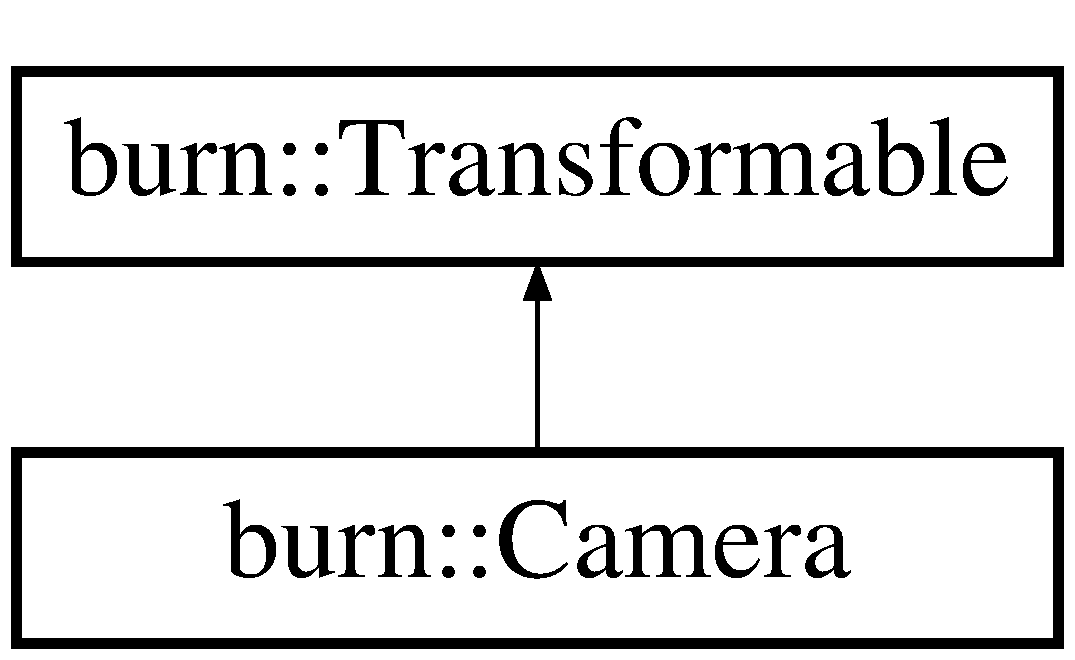
\includegraphics[height=2.000000cm]{classburn_1_1_camera}
\end{center}
\end{figure}
\subsection*{Public Member Functions}
\begin{DoxyCompactItemize}
\item 
\hyperlink{classburn_1_1_camera_aa0eac6e197cfbebe709b524eae890a02}{Camera} ()
\begin{DoxyCompactList}\small\item\em Default Contstructor of \hyperlink{classburn_1_1_camera}{Camera}. Default values\-: \end{DoxyCompactList}\item 
\hyperlink{classburn_1_1_camera_a717df173cafcdce81c01eb6744332ae7}{$\sim$\-Camera} ()
\begin{DoxyCompactList}\small\item\em Default Destructor. \end{DoxyCompactList}\item 
void \hyperlink{classburn_1_1_camera_ac3ebe6eb9c44fe8068e397c8e22b5c72}{set\-Aspect\-Ratio} (const float \&aspect\-Ratio)
\begin{DoxyCompactList}\small\item\em Changes the aspectratio that the scene will be drawn with. \end{DoxyCompactList}\item 
const float \& \hyperlink{classburn_1_1_camera_a0867612bbd199c663e477ffe68e989f6}{get\-Aspect\-Ratio} () const 
\begin{DoxyCompactList}\small\item\em Returns the current aspectratio. \end{DoxyCompactList}\item 
void \hyperlink{classburn_1_1_camera_aacfbde225b770a51a020ec15403b1c41}{look\-At} (const \hyperlink{namespaceburn_afdd7cfb352b9612432faf6947b6fff74}{Vector3f} \&point)
\begin{DoxyCompactList}\small\item\em Sets the point the camera will face to. \end{DoxyCompactList}\item 
const \hyperlink{namespaceburn_afdd7cfb352b9612432faf6947b6fff74}{Vector3f} \& \hyperlink{classburn_1_1_camera_a6e2e4ace192d77e5a9d9b62d2c2915da}{get\-Look\-At} () const 
\begin{DoxyCompactList}\small\item\em Returns the point the camera is facing. \end{DoxyCompactList}\item 
void \hyperlink{classburn_1_1_camera_a075d0fa32315aa3b9c55a2fa5135bdfd}{set\-Fov} (const float \&fov)
\begin{DoxyCompactList}\small\item\em Sets the Field-\/\-Of-\/\-View. \end{DoxyCompactList}\item 
const float \& \hyperlink{classburn_1_1_camera_ac74fe26c2f2b0d762e5886fa8ab1f97f}{get\-Fov} () const 
\begin{DoxyCompactList}\small\item\em Returns the current Field-\/\-Of-\/\-View. \end{DoxyCompactList}\end{DoxyCompactItemize}
\subsection*{Additional Inherited Members}


\subsection{Constructor \& Destructor Documentation}
\hypertarget{classburn_1_1_camera_aa0eac6e197cfbebe709b524eae890a02}{\index{burn\-::\-Camera@{burn\-::\-Camera}!Camera@{Camera}}
\index{Camera@{Camera}!burn::Camera@{burn\-::\-Camera}}
\subsubsection[{Camera}]{\setlength{\rightskip}{0pt plus 5cm}burn\-::\-Camera\-::\-Camera (
\begin{DoxyParamCaption}
{}
\end{DoxyParamCaption}
)}}\label{classburn_1_1_camera_aa0eac6e197cfbebe709b524eae890a02}


Default Contstructor of \hyperlink{classburn_1_1_camera}{Camera}. Default values\-: 


\begin{DoxyItemize}
\item Aspect\-Ratio\-: 16/9
\item Look\-At\-: 0/0/0 (Origin)
\item F\-O\-V\-: 45
\end{DoxyItemize}

\begin{DoxyNote}{Note}
In order to see results by changing values, ensure that your camera is active. 
\end{DoxyNote}
\hypertarget{classburn_1_1_camera_a717df173cafcdce81c01eb6744332ae7}{\index{burn\-::\-Camera@{burn\-::\-Camera}!$\sim$\-Camera@{$\sim$\-Camera}}
\index{$\sim$\-Camera@{$\sim$\-Camera}!burn::Camera@{burn\-::\-Camera}}
\subsubsection[{$\sim$\-Camera}]{\setlength{\rightskip}{0pt plus 5cm}burn\-::\-Camera\-::$\sim$\-Camera (
\begin{DoxyParamCaption}
{}
\end{DoxyParamCaption}
)}}\label{classburn_1_1_camera_a717df173cafcdce81c01eb6744332ae7}


Default Destructor. 

\begin{DoxyNote}{Note}
Make sure to delete the camera with Scene\-::remove\-Camera() when you have created it with Scene\-::create\-Camera() ! 
\end{DoxyNote}


\subsection{Member Function Documentation}
\hypertarget{classburn_1_1_camera_a0867612bbd199c663e477ffe68e989f6}{\index{burn\-::\-Camera@{burn\-::\-Camera}!get\-Aspect\-Ratio@{get\-Aspect\-Ratio}}
\index{get\-Aspect\-Ratio@{get\-Aspect\-Ratio}!burn::Camera@{burn\-::\-Camera}}
\subsubsection[{get\-Aspect\-Ratio}]{\setlength{\rightskip}{0pt plus 5cm}const float\& burn\-::\-Camera\-::get\-Aspect\-Ratio (
\begin{DoxyParamCaption}
{}
\end{DoxyParamCaption}
) const}}\label{classburn_1_1_camera_a0867612bbd199c663e477ffe68e989f6}


Returns the current aspectratio. 

\begin{DoxyReturn}{Returns}
The current Aspect\-Ratio
\end{DoxyReturn}
\hyperlink{classburn_1_1_camera_ac3ebe6eb9c44fe8068e397c8e22b5c72}{set\-Aspect\-Ratio()} \hypertarget{classburn_1_1_camera_ac74fe26c2f2b0d762e5886fa8ab1f97f}{\index{burn\-::\-Camera@{burn\-::\-Camera}!get\-Fov@{get\-Fov}}
\index{get\-Fov@{get\-Fov}!burn::Camera@{burn\-::\-Camera}}
\subsubsection[{get\-Fov}]{\setlength{\rightskip}{0pt plus 5cm}const float\& burn\-::\-Camera\-::get\-Fov (
\begin{DoxyParamCaption}
{}
\end{DoxyParamCaption}
) const}}\label{classburn_1_1_camera_ac74fe26c2f2b0d762e5886fa8ab1f97f}


Returns the current Field-\/\-Of-\/\-View. 

\begin{DoxyReturn}{Returns}
A value between 0 and 90 
\end{DoxyReturn}
\hypertarget{classburn_1_1_camera_a6e2e4ace192d77e5a9d9b62d2c2915da}{\index{burn\-::\-Camera@{burn\-::\-Camera}!get\-Look\-At@{get\-Look\-At}}
\index{get\-Look\-At@{get\-Look\-At}!burn::Camera@{burn\-::\-Camera}}
\subsubsection[{get\-Look\-At}]{\setlength{\rightskip}{0pt plus 5cm}const {\bf Vector3f}\& burn\-::\-Camera\-::get\-Look\-At (
\begin{DoxyParamCaption}
{}
\end{DoxyParamCaption}
) const}}\label{classburn_1_1_camera_a6e2e4ace192d77e5a9d9b62d2c2915da}


Returns the point the camera is facing. 

\begin{DoxyReturn}{Returns}
A Vector3f defining the faced point
\end{DoxyReturn}
\begin{DoxySeeAlso}{See Also}
\hyperlink{classburn_1_1_camera_aacfbde225b770a51a020ec15403b1c41}{look\-At()} 
\end{DoxySeeAlso}
\hypertarget{classburn_1_1_camera_aacfbde225b770a51a020ec15403b1c41}{\index{burn\-::\-Camera@{burn\-::\-Camera}!look\-At@{look\-At}}
\index{look\-At@{look\-At}!burn::Camera@{burn\-::\-Camera}}
\subsubsection[{look\-At}]{\setlength{\rightskip}{0pt plus 5cm}void burn\-::\-Camera\-::look\-At (
\begin{DoxyParamCaption}
\item[{const {\bf Vector3f} \&}]{point}
\end{DoxyParamCaption}
)}}\label{classburn_1_1_camera_aacfbde225b770a51a020ec15403b1c41}


Sets the point the camera will face to. 


\begin{DoxyParams}{Parameters}
{\em point} & A Vector3f defining the faced point\\
\hline
\end{DoxyParams}
\begin{DoxySeeAlso}{See Also}
\hyperlink{classburn_1_1_camera_a6e2e4ace192d77e5a9d9b62d2c2915da}{get\-Look\-At()} 
\end{DoxySeeAlso}
\hypertarget{classburn_1_1_camera_ac3ebe6eb9c44fe8068e397c8e22b5c72}{\index{burn\-::\-Camera@{burn\-::\-Camera}!set\-Aspect\-Ratio@{set\-Aspect\-Ratio}}
\index{set\-Aspect\-Ratio@{set\-Aspect\-Ratio}!burn::Camera@{burn\-::\-Camera}}
\subsubsection[{set\-Aspect\-Ratio}]{\setlength{\rightskip}{0pt plus 5cm}void burn\-::\-Camera\-::set\-Aspect\-Ratio (
\begin{DoxyParamCaption}
\item[{const float \&}]{aspect\-Ratio}
\end{DoxyParamCaption}
)}}\label{classburn_1_1_camera_ac3ebe6eb9c44fe8068e397c8e22b5c72}


Changes the aspectratio that the scene will be drawn with. 


\begin{DoxyParams}{Parameters}
{\em aspect\-Ratio} & The Aspect\-Ratio. Usually the width/height of the \hyperlink{classburn_1_1_window}{Window}\\
\hline
\end{DoxyParams}
\begin{DoxyNote}{Note}
Make sure to set your camera as active in order to see results.
\end{DoxyNote}
\begin{DoxySeeAlso}{See Also}
\hyperlink{classburn_1_1_camera_ac3ebe6eb9c44fe8068e397c8e22b5c72}{set\-Aspect\-Ratio()} 
\end{DoxySeeAlso}
\hypertarget{classburn_1_1_camera_a075d0fa32315aa3b9c55a2fa5135bdfd}{\index{burn\-::\-Camera@{burn\-::\-Camera}!set\-Fov@{set\-Fov}}
\index{set\-Fov@{set\-Fov}!burn::Camera@{burn\-::\-Camera}}
\subsubsection[{set\-Fov}]{\setlength{\rightskip}{0pt plus 5cm}void burn\-::\-Camera\-::set\-Fov (
\begin{DoxyParamCaption}
\item[{const float \&}]{fov}
\end{DoxyParamCaption}
)}}\label{classburn_1_1_camera_a075d0fa32315aa3b9c55a2fa5135bdfd}


Sets the Field-\/\-Of-\/\-View. 


\begin{DoxyParams}{Parameters}
{\em fov} & A value between 0 and 90 \\
\hline
\end{DoxyParams}


The documentation for this class was generated from the following file\-:\begin{DoxyCompactItemize}
\item 
include/\-Burngine/\-Graphics/\-Scene/\hyperlink{_camera_8h}{Camera.\-h}\end{DoxyCompactItemize}

\hypertarget{classburn_1_1_material}{\section{burn\-:\-:Material Class Reference}
\label{classburn_1_1_material}\index{burn\-::\-Material@{burn\-::\-Material}}
}


{\ttfamily \#include $<$Material.\-h$>$}

\subsection*{Public Types}
\begin{DoxyCompactItemize}
\item 
enum \hyperlink{classburn_1_1_material_a704108f8bb133e1911495b84bd0826b8}{Flag} \{ \hyperlink{classburn_1_1_material_a704108f8bb133e1911495b84bd0826b8a20ce785514749ab3909bc895127e2823}{L\-I\-G\-H\-T\-I\-N\-G} = 0, 
\hyperlink{classburn_1_1_material_a704108f8bb133e1911495b84bd0826b8a76028dd1ab583178b4e69a0894260c78}{C\-O\-U\-N\-T}
 \}
\item 
enum \hyperlink{classburn_1_1_material_a2d219315cf05e59bbffe8e3831cc6c43}{Type} \{ \hyperlink{classburn_1_1_material_a2d219315cf05e59bbffe8e3831cc6c43ae346efa71a38eb8fcbcba453a89c6aa4}{S\-O\-L\-I\-D\-\_\-\-C\-O\-L\-O\-R} = 0, 
\hyperlink{classburn_1_1_material_a2d219315cf05e59bbffe8e3831cc6c43a56549fc4dfe95a8e1fbb6bb48560f084}{T\-E\-X\-T\-U\-R\-E\-D}
 \}
\end{DoxyCompactItemize}
\subsection*{Public Member Functions}
\begin{DoxyCompactItemize}
\item 
\hyperlink{classburn_1_1_material_a790cff05e96bd7956582777754a56a34}{Material} ()
\begin{DoxyCompactList}\small\item\em The default constructor Default values\-: \end{DoxyCompactList}\item 
\hyperlink{classburn_1_1_material_a449723d0d12182275e5d0d8a6a01f41d}{$\sim$\-Material} ()
\begin{DoxyCompactList}\small\item\em The default destructor. \end{DoxyCompactList}\item 
void \hyperlink{classburn_1_1_material_a833037afe81bc0aa52ceb4581b66087f}{set\-Flag} (\hyperlink{classburn_1_1_material_a704108f8bb133e1911495b84bd0826b8}{Flag} flag, bool enabled=true)
\begin{DoxyCompactList}\small\item\em Sets the specified flag on true or false. \end{DoxyCompactList}\item 
void \hyperlink{classburn_1_1_material_a287ad604c643dc76fc07d27b45ceecd2}{set\-Type} (\hyperlink{classburn_1_1_material_a2d219315cf05e59bbffe8e3831cc6c43}{Type} type)
\begin{DoxyCompactList}\small\item\em Sets the type of the material. The \hyperlink{classburn_1_1_scene_node}{Scene\-Node} will choose the right \hyperlink{classburn_1_1_shader}{Shader}. \end{DoxyCompactList}\item 
const \hyperlink{classburn_1_1_material_a2d219315cf05e59bbffe8e3831cc6c43}{Type} \& \hyperlink{classburn_1_1_material_afce65f6bded42bd03552741fe70649d8}{get\-Type} () const 
\begin{DoxyCompactList}\small\item\em Returns the current type. \end{DoxyCompactList}\item 
bool \hyperlink{classburn_1_1_material_afa32027c9de752c96b74e08b3f1e42af}{is\-Flag\-Set} (\hyperlink{classburn_1_1_material_a704108f8bb133e1911495b84bd0826b8}{Flag} flag) const 
\begin{DoxyCompactList}\small\item\em Returns the current status of a flag. \end{DoxyCompactList}\item 
void \hyperlink{classburn_1_1_material_ae50bc615e9bb17bc9eb232345fb1e776}{set\-Specular\-Color} (const \hyperlink{namespaceburn_afdd7cfb352b9612432faf6947b6fff74}{Vector3f} \&color)
\item 
const \hyperlink{namespaceburn_afdd7cfb352b9612432faf6947b6fff74}{Vector3f} \& \hyperlink{classburn_1_1_material_ab7d639a776c308b57eb0b3210b27449e}{get\-Specular\-Color} () const 
\item 
void \hyperlink{classburn_1_1_material_a0b50c4daafb286d54d5159bc93fc695c}{set\-Diffuse\-Color} (const \hyperlink{namespaceburn_afdd7cfb352b9612432faf6947b6fff74}{Vector3f} \&color)
\item 
const \hyperlink{namespaceburn_afdd7cfb352b9612432faf6947b6fff74}{Vector3f} \& \hyperlink{classburn_1_1_material_acc1501d3c24c0bf6c2f120d1e1a67c0f}{get\-Diffuse\-Color} () const 
\item 
void \hyperlink{classburn_1_1_material_a730e2d8f5d444f6ce45e1f25a4f424d6}{set\-Index} (const unsigned int \&index)
\item 
const unsigned int \& \hyperlink{classburn_1_1_material_a7e30e5e26a8a9648910ef17901452d20}{get\-Index} () const 
\item 
void \hyperlink{classburn_1_1_material_a016895c77f4fd7393ab263ac7455e5a2}{use\-Diffuse\-Color} (bool should\-Use\-Diffuse=true)
\item 
bool \hyperlink{classburn_1_1_material_a4f2d46a41409a068985c7377eeb1f3c4}{is\-Using\-Diffuse\-Color} () const 
\end{DoxyCompactItemize}


\subsection{Member Enumeration Documentation}
\hypertarget{classburn_1_1_material_a704108f8bb133e1911495b84bd0826b8}{\index{burn\-::\-Material@{burn\-::\-Material}!Flag@{Flag}}
\index{Flag@{Flag}!burn::Material@{burn\-::\-Material}}
\subsubsection[{Flag}]{\setlength{\rightskip}{0pt plus 5cm}enum {\bf burn\-::\-Material\-::\-Flag}}}\label{classburn_1_1_material_a704108f8bb133e1911495b84bd0826b8}
\begin{Desc}
\item[Enumerator]\par
\begin{description}
\index{L\-I\-G\-H\-T\-I\-N\-G@{L\-I\-G\-H\-T\-I\-N\-G}!burn\-::\-Material@{burn\-::\-Material}}\index{burn\-::\-Material@{burn\-::\-Material}!L\-I\-G\-H\-T\-I\-N\-G@{L\-I\-G\-H\-T\-I\-N\-G}}\item[{\em 
\hypertarget{classburn_1_1_material_a704108f8bb133e1911495b84bd0826b8a20ce785514749ab3909bc895127e2823}{L\-I\-G\-H\-T\-I\-N\-G}\label{classburn_1_1_material_a704108f8bb133e1911495b84bd0826b8a20ce785514749ab3909bc895127e2823}
}]\index{C\-O\-U\-N\-T@{C\-O\-U\-N\-T}!burn\-::\-Material@{burn\-::\-Material}}\index{burn\-::\-Material@{burn\-::\-Material}!C\-O\-U\-N\-T@{C\-O\-U\-N\-T}}\item[{\em 
\hypertarget{classburn_1_1_material_a704108f8bb133e1911495b84bd0826b8a76028dd1ab583178b4e69a0894260c78}{C\-O\-U\-N\-T}\label{classburn_1_1_material_a704108f8bb133e1911495b84bd0826b8a76028dd1ab583178b4e69a0894260c78}
}]\end{description}
\end{Desc}
\hypertarget{classburn_1_1_material_a2d219315cf05e59bbffe8e3831cc6c43}{\index{burn\-::\-Material@{burn\-::\-Material}!Type@{Type}}
\index{Type@{Type}!burn::Material@{burn\-::\-Material}}
\subsubsection[{Type}]{\setlength{\rightskip}{0pt plus 5cm}enum {\bf burn\-::\-Material\-::\-Type}}}\label{classburn_1_1_material_a2d219315cf05e59bbffe8e3831cc6c43}
\begin{Desc}
\item[Enumerator]\par
\begin{description}
\index{S\-O\-L\-I\-D\-\_\-\-C\-O\-L\-O\-R@{S\-O\-L\-I\-D\-\_\-\-C\-O\-L\-O\-R}!burn\-::\-Material@{burn\-::\-Material}}\index{burn\-::\-Material@{burn\-::\-Material}!S\-O\-L\-I\-D\-\_\-\-C\-O\-L\-O\-R@{S\-O\-L\-I\-D\-\_\-\-C\-O\-L\-O\-R}}\item[{\em 
\hypertarget{classburn_1_1_material_a2d219315cf05e59bbffe8e3831cc6c43ae346efa71a38eb8fcbcba453a89c6aa4}{S\-O\-L\-I\-D\-\_\-\-C\-O\-L\-O\-R}\label{classburn_1_1_material_a2d219315cf05e59bbffe8e3831cc6c43ae346efa71a38eb8fcbcba453a89c6aa4}
}]\index{T\-E\-X\-T\-U\-R\-E\-D@{T\-E\-X\-T\-U\-R\-E\-D}!burn\-::\-Material@{burn\-::\-Material}}\index{burn\-::\-Material@{burn\-::\-Material}!T\-E\-X\-T\-U\-R\-E\-D@{T\-E\-X\-T\-U\-R\-E\-D}}\item[{\em 
\hypertarget{classburn_1_1_material_a2d219315cf05e59bbffe8e3831cc6c43a56549fc4dfe95a8e1fbb6bb48560f084}{T\-E\-X\-T\-U\-R\-E\-D}\label{classburn_1_1_material_a2d219315cf05e59bbffe8e3831cc6c43a56549fc4dfe95a8e1fbb6bb48560f084}
}]\end{description}
\end{Desc}


\subsection{Constructor \& Destructor Documentation}
\hypertarget{classburn_1_1_material_a790cff05e96bd7956582777754a56a34}{\index{burn\-::\-Material@{burn\-::\-Material}!Material@{Material}}
\index{Material@{Material}!burn::Material@{burn\-::\-Material}}
\subsubsection[{Material}]{\setlength{\rightskip}{0pt plus 5cm}burn\-::\-Material\-::\-Material (
\begin{DoxyParamCaption}
{}
\end{DoxyParamCaption}
)}}\label{classburn_1_1_material_a790cff05e96bd7956582777754a56a34}


The default constructor Default values\-: 


\begin{DoxyItemize}
\item Type\-: S\-O\-L\-I\-D\-\_\-\-C\-O\-L\-O\-R
\item Flag\mbox{[}L\-I\-G\-H\-T\-I\-N\-G\mbox{]}\-: false 
\end{DoxyItemize}\hypertarget{classburn_1_1_material_a449723d0d12182275e5d0d8a6a01f41d}{\index{burn\-::\-Material@{burn\-::\-Material}!$\sim$\-Material@{$\sim$\-Material}}
\index{$\sim$\-Material@{$\sim$\-Material}!burn::Material@{burn\-::\-Material}}
\subsubsection[{$\sim$\-Material}]{\setlength{\rightskip}{0pt plus 5cm}burn\-::\-Material\-::$\sim$\-Material (
\begin{DoxyParamCaption}
{}
\end{DoxyParamCaption}
)}}\label{classburn_1_1_material_a449723d0d12182275e5d0d8a6a01f41d}


The default destructor. 



\subsection{Member Function Documentation}
\hypertarget{classburn_1_1_material_acc1501d3c24c0bf6c2f120d1e1a67c0f}{\index{burn\-::\-Material@{burn\-::\-Material}!get\-Diffuse\-Color@{get\-Diffuse\-Color}}
\index{get\-Diffuse\-Color@{get\-Diffuse\-Color}!burn::Material@{burn\-::\-Material}}
\subsubsection[{get\-Diffuse\-Color}]{\setlength{\rightskip}{0pt plus 5cm}const {\bf Vector3f}\& burn\-::\-Material\-::get\-Diffuse\-Color (
\begin{DoxyParamCaption}
{}
\end{DoxyParamCaption}
) const}}\label{classburn_1_1_material_acc1501d3c24c0bf6c2f120d1e1a67c0f}
\hypertarget{classburn_1_1_material_a7e30e5e26a8a9648910ef17901452d20}{\index{burn\-::\-Material@{burn\-::\-Material}!get\-Index@{get\-Index}}
\index{get\-Index@{get\-Index}!burn::Material@{burn\-::\-Material}}
\subsubsection[{get\-Index}]{\setlength{\rightskip}{0pt plus 5cm}const unsigned int\& burn\-::\-Material\-::get\-Index (
\begin{DoxyParamCaption}
{}
\end{DoxyParamCaption}
) const}}\label{classburn_1_1_material_a7e30e5e26a8a9648910ef17901452d20}
\hypertarget{classburn_1_1_material_ab7d639a776c308b57eb0b3210b27449e}{\index{burn\-::\-Material@{burn\-::\-Material}!get\-Specular\-Color@{get\-Specular\-Color}}
\index{get\-Specular\-Color@{get\-Specular\-Color}!burn::Material@{burn\-::\-Material}}
\subsubsection[{get\-Specular\-Color}]{\setlength{\rightskip}{0pt plus 5cm}const {\bf Vector3f}\& burn\-::\-Material\-::get\-Specular\-Color (
\begin{DoxyParamCaption}
{}
\end{DoxyParamCaption}
) const}}\label{classburn_1_1_material_ab7d639a776c308b57eb0b3210b27449e}
\hypertarget{classburn_1_1_material_afce65f6bded42bd03552741fe70649d8}{\index{burn\-::\-Material@{burn\-::\-Material}!get\-Type@{get\-Type}}
\index{get\-Type@{get\-Type}!burn::Material@{burn\-::\-Material}}
\subsubsection[{get\-Type}]{\setlength{\rightskip}{0pt plus 5cm}const {\bf Type}\& burn\-::\-Material\-::get\-Type (
\begin{DoxyParamCaption}
{}
\end{DoxyParamCaption}
) const}}\label{classburn_1_1_material_afce65f6bded42bd03552741fe70649d8}


Returns the current type. 

\begin{DoxyReturn}{Returns}
The current materialtype
\end{DoxyReturn}
\begin{DoxySeeAlso}{See Also}
\hyperlink{classburn_1_1_material_a287ad604c643dc76fc07d27b45ceecd2}{set\-Type()} 
\end{DoxySeeAlso}
\hypertarget{classburn_1_1_material_afa32027c9de752c96b74e08b3f1e42af}{\index{burn\-::\-Material@{burn\-::\-Material}!is\-Flag\-Set@{is\-Flag\-Set}}
\index{is\-Flag\-Set@{is\-Flag\-Set}!burn::Material@{burn\-::\-Material}}
\subsubsection[{is\-Flag\-Set}]{\setlength{\rightskip}{0pt plus 5cm}bool burn\-::\-Material\-::is\-Flag\-Set (
\begin{DoxyParamCaption}
\item[{{\bf Flag}}]{flag}
\end{DoxyParamCaption}
) const}}\label{classburn_1_1_material_afa32027c9de752c96b74e08b3f1e42af}


Returns the current status of a flag. 


\begin{DoxyParams}{Parameters}
{\em flag} & The flag to check\\
\hline
\end{DoxyParams}
\begin{DoxyReturn}{Returns}
Status of a flag.
\end{DoxyReturn}
\begin{DoxySeeAlso}{See Also}
\hyperlink{classburn_1_1_material_a833037afe81bc0aa52ceb4581b66087f}{set\-Flag()} 
\end{DoxySeeAlso}
\hypertarget{classburn_1_1_material_a4f2d46a41409a068985c7377eeb1f3c4}{\index{burn\-::\-Material@{burn\-::\-Material}!is\-Using\-Diffuse\-Color@{is\-Using\-Diffuse\-Color}}
\index{is\-Using\-Diffuse\-Color@{is\-Using\-Diffuse\-Color}!burn::Material@{burn\-::\-Material}}
\subsubsection[{is\-Using\-Diffuse\-Color}]{\setlength{\rightskip}{0pt plus 5cm}bool burn\-::\-Material\-::is\-Using\-Diffuse\-Color (
\begin{DoxyParamCaption}
{}
\end{DoxyParamCaption}
) const}}\label{classburn_1_1_material_a4f2d46a41409a068985c7377eeb1f3c4}
\hypertarget{classburn_1_1_material_a0b50c4daafb286d54d5159bc93fc695c}{\index{burn\-::\-Material@{burn\-::\-Material}!set\-Diffuse\-Color@{set\-Diffuse\-Color}}
\index{set\-Diffuse\-Color@{set\-Diffuse\-Color}!burn::Material@{burn\-::\-Material}}
\subsubsection[{set\-Diffuse\-Color}]{\setlength{\rightskip}{0pt plus 5cm}void burn\-::\-Material\-::set\-Diffuse\-Color (
\begin{DoxyParamCaption}
\item[{const {\bf Vector3f} \&}]{color}
\end{DoxyParamCaption}
)}}\label{classburn_1_1_material_a0b50c4daafb286d54d5159bc93fc695c}
\hypertarget{classburn_1_1_material_a833037afe81bc0aa52ceb4581b66087f}{\index{burn\-::\-Material@{burn\-::\-Material}!set\-Flag@{set\-Flag}}
\index{set\-Flag@{set\-Flag}!burn::Material@{burn\-::\-Material}}
\subsubsection[{set\-Flag}]{\setlength{\rightskip}{0pt plus 5cm}void burn\-::\-Material\-::set\-Flag (
\begin{DoxyParamCaption}
\item[{{\bf Flag}}]{flag, }
\item[{bool}]{enabled = {\ttfamily true}}
\end{DoxyParamCaption}
)}}\label{classburn_1_1_material_a833037afe81bc0aa52ceb4581b66087f}


Sets the specified flag on true or false. 


\begin{DoxyParams}{Parameters}
{\em flag} & The flag to set \\
\hline
{\em enabled} & Sets the specified flag on true or false\\
\hline
\end{DoxyParams}
\begin{DoxySeeAlso}{See Also}
\hyperlink{classburn_1_1_material_afa32027c9de752c96b74e08b3f1e42af}{is\-Flag\-Set()} 
\end{DoxySeeAlso}
\hypertarget{classburn_1_1_material_a730e2d8f5d444f6ce45e1f25a4f424d6}{\index{burn\-::\-Material@{burn\-::\-Material}!set\-Index@{set\-Index}}
\index{set\-Index@{set\-Index}!burn::Material@{burn\-::\-Material}}
\subsubsection[{set\-Index}]{\setlength{\rightskip}{0pt plus 5cm}void burn\-::\-Material\-::set\-Index (
\begin{DoxyParamCaption}
\item[{const unsigned int \&}]{index}
\end{DoxyParamCaption}
)}}\label{classburn_1_1_material_a730e2d8f5d444f6ce45e1f25a4f424d6}
\hypertarget{classburn_1_1_material_ae50bc615e9bb17bc9eb232345fb1e776}{\index{burn\-::\-Material@{burn\-::\-Material}!set\-Specular\-Color@{set\-Specular\-Color}}
\index{set\-Specular\-Color@{set\-Specular\-Color}!burn::Material@{burn\-::\-Material}}
\subsubsection[{set\-Specular\-Color}]{\setlength{\rightskip}{0pt plus 5cm}void burn\-::\-Material\-::set\-Specular\-Color (
\begin{DoxyParamCaption}
\item[{const {\bf Vector3f} \&}]{color}
\end{DoxyParamCaption}
)}}\label{classburn_1_1_material_ae50bc615e9bb17bc9eb232345fb1e776}
\hypertarget{classburn_1_1_material_a287ad604c643dc76fc07d27b45ceecd2}{\index{burn\-::\-Material@{burn\-::\-Material}!set\-Type@{set\-Type}}
\index{set\-Type@{set\-Type}!burn::Material@{burn\-::\-Material}}
\subsubsection[{set\-Type}]{\setlength{\rightskip}{0pt plus 5cm}void burn\-::\-Material\-::set\-Type (
\begin{DoxyParamCaption}
\item[{{\bf Type}}]{type}
\end{DoxyParamCaption}
)}}\label{classburn_1_1_material_a287ad604c643dc76fc07d27b45ceecd2}


Sets the type of the material. The \hyperlink{classburn_1_1_scene_node}{Scene\-Node} will choose the right \hyperlink{classburn_1_1_shader}{Shader}. 


\begin{DoxyParams}{Parameters}
{\em type} & The materialtype.\\
\hline
\end{DoxyParams}
\begin{DoxySeeAlso}{See Also}
\hyperlink{classburn_1_1_material_afce65f6bded42bd03552741fe70649d8}{get\-Type()}
\end{DoxySeeAlso}
\begin{DoxyNote}{Note}
Ensure that you have loaded the \hyperlink{structburn_1_1_burngine_shaders}{Burngine\-Shaders} before renering. E.\-g. by calling Burngine\-Shaders\-::load\-All\-Shaders() 
\end{DoxyNote}
\hypertarget{classburn_1_1_material_a016895c77f4fd7393ab263ac7455e5a2}{\index{burn\-::\-Material@{burn\-::\-Material}!use\-Diffuse\-Color@{use\-Diffuse\-Color}}
\index{use\-Diffuse\-Color@{use\-Diffuse\-Color}!burn::Material@{burn\-::\-Material}}
\subsubsection[{use\-Diffuse\-Color}]{\setlength{\rightskip}{0pt plus 5cm}void burn\-::\-Material\-::use\-Diffuse\-Color (
\begin{DoxyParamCaption}
\item[{bool}]{should\-Use\-Diffuse = {\ttfamily true}}
\end{DoxyParamCaption}
)}}\label{classburn_1_1_material_a016895c77f4fd7393ab263ac7455e5a2}


The documentation for this class was generated from the following file\-:\begin{DoxyCompactItemize}
\item 
include/\-Burngine/\-Graphics/\-Scene/\hyperlink{_material_8h}{Material.\-h}\end{DoxyCompactItemize}

\hypertarget{classburn_1_1_mesh}{\section{burn\-:\-:Mesh Class Reference}
\label{classburn_1_1_mesh}\index{burn\-::\-Mesh@{burn\-::\-Mesh}}
}


{\ttfamily \#include $<$Mesh.\-h$>$}

\subsection*{Public Member Functions}
\begin{DoxyCompactItemize}
\item 
\hyperlink{classburn_1_1_mesh_a35d4706a490d0f2bb190b6b785621e07}{Mesh} ()
\begin{DoxyCompactList}\small\item\em The default constructor. \end{DoxyCompactList}\item 
\hyperlink{classburn_1_1_mesh_ad8b2e6283ea14b3943a8945ab7f2d27d}{$\sim$\-Mesh} ()
\begin{DoxyCompactList}\small\item\em The default destructor. \end{DoxyCompactList}\item 
bool \hyperlink{classburn_1_1_mesh_a3179d5730bfcf0e781b1c0daebfc7439}{load\-From\-File} (const std\-::string \&file)
\begin{DoxyCompactList}\small\item\em Loads a 3\-D-\/model into the \hyperlink{classburn_1_1_mesh}{Mesh} object. It uses the assimp importer, so it supports the files that assimp does. \end{DoxyCompactList}\item 
void \hyperlink{classburn_1_1_mesh_ae0996bd5d561cdf7b26e27c713facea7}{set\-Vertices} (const std\-::vector$<$ \hyperlink{classburn_1_1_vertex}{Vertex} $>$ \&vertices)
\begin{DoxyCompactList}\small\item\em Sets the vertices of the mesh, so that they can be used for rendering later on. \end{DoxyCompactList}\item 
size\-\_\-t \hyperlink{classburn_1_1_mesh_a076016c8452ff794880480626394e44c}{get\-Vertex\-Count} () const 
\begin{DoxyCompactList}\small\item\em Returns the count of the vertices which the mesh is holding. \end{DoxyCompactList}\item 
const G\-Luint \& \hyperlink{classburn_1_1_mesh_a617b88d25c58c342f02751d67cb5e29b}{get\-Position\-Buffer} () const 
\begin{DoxyCompactList}\small\item\em Returns the id of the position-\/buffer. This is used mostly internally. But you can check the buffer by comparing the returned value with 0. \end{DoxyCompactList}\item 
const G\-Luint \& \hyperlink{classburn_1_1_mesh_ad571f57e9a162b86585c0b3f288bbfc6}{get\-Normal\-Buffer} () const 
\begin{DoxyCompactList}\small\item\em Returns the id of the normal-\/buffer. This is used mostly internally. But you can check the buffer by comparing the returned value with 0. \end{DoxyCompactList}\item 
const G\-Luint \& \hyperlink{classburn_1_1_mesh_ae8757bde80c135f9d8e8e0291e00ffe5}{get\-Color\-Buffer} () const 
\begin{DoxyCompactList}\small\item\em Returns the id of the color-\/buffer. This is used mostly internally. But you can check the buffer by comparing the returned value with 0. \end{DoxyCompactList}\item 
const G\-Luint \& \hyperlink{classburn_1_1_mesh_a5bcc126c9f06b9f04549b02328f2fc72}{get\-Uv\-Buffer} () const 
\begin{DoxyCompactList}\small\item\em Returns the id of the U\-V-\/buffer. This is used mostly internally. But you can check the buffer by comparing the returned value with 0. \end{DoxyCompactList}\item 
void \hyperlink{classburn_1_1_mesh_a2457c00cd236e5933e725bb1d55db0d9}{set\-Texture} (const \hyperlink{classburn_1_1_texture}{Texture} \&texture)
\begin{DoxyCompactList}\small\item\em Sets the \hyperlink{classburn_1_1_texture}{Texture} of the mesh. \end{DoxyCompactList}\item 
const \hyperlink{classburn_1_1_texture}{Texture} \& \hyperlink{classburn_1_1_mesh_acbea44f2a2683c44728bb17e4691d406}{get\-Texture} () const 
\begin{DoxyCompactList}\small\item\em Returns the current \hyperlink{classburn_1_1_texture}{Texture} of the mesh. \end{DoxyCompactList}\item 
\hyperlink{classburn_1_1_material}{Material} \& \hyperlink{classburn_1_1_mesh_a7e3f6168e3bb37e5c30323c5e19b85cc}{get\-Material} ()
\begin{DoxyCompactList}\small\item\em Returns the material that the node is using. \end{DoxyCompactList}\item 
void \hyperlink{classburn_1_1_mesh_a2ff24f1eb82cb417062e8d1ec179d8bd}{set\-Material} (\hyperlink{classburn_1_1_material}{Material} \&material)
\begin{DoxyCompactList}\small\item\em Sets the material of the node. Influences the rendering behaviour. \end{DoxyCompactList}\item 
void \hyperlink{classburn_1_1_mesh_a4880e1e9d0580cd08064290fe4c3d3a0}{update} ()
\item 
void \hyperlink{classburn_1_1_mesh_ad9d9b1c1d6a9486e65e384f28aa009d5}{force\-Update} ()
\end{DoxyCompactItemize}


\subsection{Constructor \& Destructor Documentation}
\hypertarget{classburn_1_1_mesh_a35d4706a490d0f2bb190b6b785621e07}{\index{burn\-::\-Mesh@{burn\-::\-Mesh}!Mesh@{Mesh}}
\index{Mesh@{Mesh}!burn::Mesh@{burn\-::\-Mesh}}
\subsubsection[{Mesh}]{\setlength{\rightskip}{0pt plus 5cm}burn\-::\-Mesh\-::\-Mesh (
\begin{DoxyParamCaption}
{}
\end{DoxyParamCaption}
)}}\label{classburn_1_1_mesh_a35d4706a490d0f2bb190b6b785621e07}


The default constructor. 

\hypertarget{classburn_1_1_mesh_ad8b2e6283ea14b3943a8945ab7f2d27d}{\index{burn\-::\-Mesh@{burn\-::\-Mesh}!$\sim$\-Mesh@{$\sim$\-Mesh}}
\index{$\sim$\-Mesh@{$\sim$\-Mesh}!burn::Mesh@{burn\-::\-Mesh}}
\subsubsection[{$\sim$\-Mesh}]{\setlength{\rightskip}{0pt plus 5cm}burn\-::\-Mesh\-::$\sim$\-Mesh (
\begin{DoxyParamCaption}
{}
\end{DoxyParamCaption}
)}}\label{classburn_1_1_mesh_ad8b2e6283ea14b3943a8945ab7f2d27d}


The default destructor. 



\subsection{Member Function Documentation}
\hypertarget{classburn_1_1_mesh_ad9d9b1c1d6a9486e65e384f28aa009d5}{\index{burn\-::\-Mesh@{burn\-::\-Mesh}!force\-Update@{force\-Update}}
\index{force\-Update@{force\-Update}!burn::Mesh@{burn\-::\-Mesh}}
\subsubsection[{force\-Update}]{\setlength{\rightskip}{0pt plus 5cm}void burn\-::\-Mesh\-::force\-Update (
\begin{DoxyParamCaption}
{}
\end{DoxyParamCaption}
)}}\label{classburn_1_1_mesh_ad9d9b1c1d6a9486e65e384f28aa009d5}
\hypertarget{classburn_1_1_mesh_ae8757bde80c135f9d8e8e0291e00ffe5}{\index{burn\-::\-Mesh@{burn\-::\-Mesh}!get\-Color\-Buffer@{get\-Color\-Buffer}}
\index{get\-Color\-Buffer@{get\-Color\-Buffer}!burn::Mesh@{burn\-::\-Mesh}}
\subsubsection[{get\-Color\-Buffer}]{\setlength{\rightskip}{0pt plus 5cm}const G\-Luint \& burn\-::\-Mesh\-::get\-Color\-Buffer (
\begin{DoxyParamCaption}
{}
\end{DoxyParamCaption}
) const}}\label{classburn_1_1_mesh_ae8757bde80c135f9d8e8e0291e00ffe5}


Returns the id of the color-\/buffer. This is used mostly internally. But you can check the buffer by comparing the returned value with 0. 

\begin{DoxyReturn}{Returns}
Returns the id of the color-\/buffer or 0 if no color-\/buffer exists 
\end{DoxyReturn}
\hypertarget{classburn_1_1_mesh_a7e3f6168e3bb37e5c30323c5e19b85cc}{\index{burn\-::\-Mesh@{burn\-::\-Mesh}!get\-Material@{get\-Material}}
\index{get\-Material@{get\-Material}!burn::Mesh@{burn\-::\-Mesh}}
\subsubsection[{get\-Material}]{\setlength{\rightskip}{0pt plus 5cm}{\bf Material} \& burn\-::\-Mesh\-::get\-Material (
\begin{DoxyParamCaption}
{}
\end{DoxyParamCaption}
)}}\label{classburn_1_1_mesh_a7e3f6168e3bb37e5c30323c5e19b85cc}


Returns the material that the node is using. 

\begin{DoxyReturn}{Returns}
The \hyperlink{classburn_1_1_material}{Material} of the node.
\end{DoxyReturn}
\begin{DoxySeeAlso}{See Also}
\hyperlink{classburn_1_1_mesh_a2ff24f1eb82cb417062e8d1ec179d8bd}{set\-Material()} 
\end{DoxySeeAlso}
\hypertarget{classburn_1_1_mesh_ad571f57e9a162b86585c0b3f288bbfc6}{\index{burn\-::\-Mesh@{burn\-::\-Mesh}!get\-Normal\-Buffer@{get\-Normal\-Buffer}}
\index{get\-Normal\-Buffer@{get\-Normal\-Buffer}!burn::Mesh@{burn\-::\-Mesh}}
\subsubsection[{get\-Normal\-Buffer}]{\setlength{\rightskip}{0pt plus 5cm}const G\-Luint \& burn\-::\-Mesh\-::get\-Normal\-Buffer (
\begin{DoxyParamCaption}
{}
\end{DoxyParamCaption}
) const}}\label{classburn_1_1_mesh_ad571f57e9a162b86585c0b3f288bbfc6}


Returns the id of the normal-\/buffer. This is used mostly internally. But you can check the buffer by comparing the returned value with 0. 

\begin{DoxyReturn}{Returns}
Returns the id of the normal-\/buffer or 0 if no normal-\/buffer exists 
\end{DoxyReturn}
\hypertarget{classburn_1_1_mesh_a617b88d25c58c342f02751d67cb5e29b}{\index{burn\-::\-Mesh@{burn\-::\-Mesh}!get\-Position\-Buffer@{get\-Position\-Buffer}}
\index{get\-Position\-Buffer@{get\-Position\-Buffer}!burn::Mesh@{burn\-::\-Mesh}}
\subsubsection[{get\-Position\-Buffer}]{\setlength{\rightskip}{0pt plus 5cm}const G\-Luint \& burn\-::\-Mesh\-::get\-Position\-Buffer (
\begin{DoxyParamCaption}
{}
\end{DoxyParamCaption}
) const}}\label{classburn_1_1_mesh_a617b88d25c58c342f02751d67cb5e29b}


Returns the id of the position-\/buffer. This is used mostly internally. But you can check the buffer by comparing the returned value with 0. 

\begin{DoxyReturn}{Returns}
Returns the id of the position-\/buffer or 0 if no position-\/buffer exists 
\end{DoxyReturn}
\hypertarget{classburn_1_1_mesh_acbea44f2a2683c44728bb17e4691d406}{\index{burn\-::\-Mesh@{burn\-::\-Mesh}!get\-Texture@{get\-Texture}}
\index{get\-Texture@{get\-Texture}!burn::Mesh@{burn\-::\-Mesh}}
\subsubsection[{get\-Texture}]{\setlength{\rightskip}{0pt plus 5cm}const {\bf Texture} \& burn\-::\-Mesh\-::get\-Texture (
\begin{DoxyParamCaption}
{}
\end{DoxyParamCaption}
) const}}\label{classburn_1_1_mesh_acbea44f2a2683c44728bb17e4691d406}


Returns the current \hyperlink{classburn_1_1_texture}{Texture} of the mesh. 

\begin{DoxyReturn}{Returns}
The current \hyperlink{classburn_1_1_texture}{Texture}
\end{DoxyReturn}
\begin{DoxySeeAlso}{See Also}
\hyperlink{classburn_1_1_mesh_a2457c00cd236e5933e725bb1d55db0d9}{set\-Texture()} 
\end{DoxySeeAlso}
\hypertarget{classburn_1_1_mesh_a5bcc126c9f06b9f04549b02328f2fc72}{\index{burn\-::\-Mesh@{burn\-::\-Mesh}!get\-Uv\-Buffer@{get\-Uv\-Buffer}}
\index{get\-Uv\-Buffer@{get\-Uv\-Buffer}!burn::Mesh@{burn\-::\-Mesh}}
\subsubsection[{get\-Uv\-Buffer}]{\setlength{\rightskip}{0pt plus 5cm}const G\-Luint \& burn\-::\-Mesh\-::get\-Uv\-Buffer (
\begin{DoxyParamCaption}
{}
\end{DoxyParamCaption}
) const}}\label{classburn_1_1_mesh_a5bcc126c9f06b9f04549b02328f2fc72}


Returns the id of the U\-V-\/buffer. This is used mostly internally. But you can check the buffer by comparing the returned value with 0. 

\begin{DoxyReturn}{Returns}
Returns the id of the U\-V-\/buffer or 0 if no U\-V-\/buffer exists 
\end{DoxyReturn}
\hypertarget{classburn_1_1_mesh_a076016c8452ff794880480626394e44c}{\index{burn\-::\-Mesh@{burn\-::\-Mesh}!get\-Vertex\-Count@{get\-Vertex\-Count}}
\index{get\-Vertex\-Count@{get\-Vertex\-Count}!burn::Mesh@{burn\-::\-Mesh}}
\subsubsection[{get\-Vertex\-Count}]{\setlength{\rightskip}{0pt plus 5cm}size\-\_\-t burn\-::\-Mesh\-::get\-Vertex\-Count (
\begin{DoxyParamCaption}
{}
\end{DoxyParamCaption}
) const}}\label{classburn_1_1_mesh_a076016c8452ff794880480626394e44c}


Returns the count of the vertices which the mesh is holding. 

\begin{DoxyReturn}{Returns}
The count of vertices
\end{DoxyReturn}
\begin{DoxySeeAlso}{See Also}
\hyperlink{classburn_1_1_mesh_ae0996bd5d561cdf7b26e27c713facea7}{set\-Vertices()} 
\end{DoxySeeAlso}
\hypertarget{classburn_1_1_mesh_a3179d5730bfcf0e781b1c0daebfc7439}{\index{burn\-::\-Mesh@{burn\-::\-Mesh}!load\-From\-File@{load\-From\-File}}
\index{load\-From\-File@{load\-From\-File}!burn::Mesh@{burn\-::\-Mesh}}
\subsubsection[{load\-From\-File}]{\setlength{\rightskip}{0pt plus 5cm}bool burn\-::\-Mesh\-::load\-From\-File (
\begin{DoxyParamCaption}
\item[{const std\-::string \&}]{file}
\end{DoxyParamCaption}
)}}\label{classburn_1_1_mesh_a3179d5730bfcf0e781b1c0daebfc7439}


Loads a 3\-D-\/model into the \hyperlink{classburn_1_1_mesh}{Mesh} object. It uses the assimp importer, so it supports the files that assimp does. 


\begin{DoxyParams}{Parameters}
{\em file} & The file to load\\
\hline
\end{DoxyParams}
\begin{DoxyReturn}{Returns}
Returns true on load-\/success 
\end{DoxyReturn}
\hypertarget{classburn_1_1_mesh_a2ff24f1eb82cb417062e8d1ec179d8bd}{\index{burn\-::\-Mesh@{burn\-::\-Mesh}!set\-Material@{set\-Material}}
\index{set\-Material@{set\-Material}!burn::Mesh@{burn\-::\-Mesh}}
\subsubsection[{set\-Material}]{\setlength{\rightskip}{0pt plus 5cm}void burn\-::\-Mesh\-::set\-Material (
\begin{DoxyParamCaption}
\item[{{\bf Material} \&}]{material}
\end{DoxyParamCaption}
)}}\label{classburn_1_1_mesh_a2ff24f1eb82cb417062e8d1ec179d8bd}


Sets the material of the node. Influences the rendering behaviour. 


\begin{DoxyParams}{Parameters}
{\em material} & The \hyperlink{classburn_1_1_material}{Material} to use.\\
\hline
\end{DoxyParams}
\begin{DoxySeeAlso}{See Also}
\hyperlink{classburn_1_1_mesh_a7e3f6168e3bb37e5c30323c5e19b85cc}{get\-Material()} 
\end{DoxySeeAlso}
\hypertarget{classburn_1_1_mesh_a2457c00cd236e5933e725bb1d55db0d9}{\index{burn\-::\-Mesh@{burn\-::\-Mesh}!set\-Texture@{set\-Texture}}
\index{set\-Texture@{set\-Texture}!burn::Mesh@{burn\-::\-Mesh}}
\subsubsection[{set\-Texture}]{\setlength{\rightskip}{0pt plus 5cm}void burn\-::\-Mesh\-::set\-Texture (
\begin{DoxyParamCaption}
\item[{const {\bf Texture} \&}]{texture}
\end{DoxyParamCaption}
)}}\label{classburn_1_1_mesh_a2457c00cd236e5933e725bb1d55db0d9}


Sets the \hyperlink{classburn_1_1_texture}{Texture} of the mesh. 


\begin{DoxyParams}{Parameters}
{\em texture} & The \hyperlink{classburn_1_1_texture}{Texture} to set\\
\hline
\end{DoxyParams}
\begin{DoxySeeAlso}{See Also}
\hyperlink{classburn_1_1_mesh_acbea44f2a2683c44728bb17e4691d406}{get\-Texture()} 
\end{DoxySeeAlso}
\hypertarget{classburn_1_1_mesh_ae0996bd5d561cdf7b26e27c713facea7}{\index{burn\-::\-Mesh@{burn\-::\-Mesh}!set\-Vertices@{set\-Vertices}}
\index{set\-Vertices@{set\-Vertices}!burn::Mesh@{burn\-::\-Mesh}}
\subsubsection[{set\-Vertices}]{\setlength{\rightskip}{0pt plus 5cm}void burn\-::\-Mesh\-::set\-Vertices (
\begin{DoxyParamCaption}
\item[{const std\-::vector$<$ {\bf Vertex} $>$ \&}]{vertices}
\end{DoxyParamCaption}
)}}\label{classburn_1_1_mesh_ae0996bd5d561cdf7b26e27c713facea7}


Sets the vertices of the mesh, so that they can be used for rendering later on. 


\begin{DoxyParams}{Parameters}
{\em vertices} & A vector with vertices\\
\hline
\end{DoxyParams}
\begin{DoxySeeAlso}{See Also}
\hyperlink{classburn_1_1_vertex}{Vertex} 
\end{DoxySeeAlso}
\hypertarget{classburn_1_1_mesh_a4880e1e9d0580cd08064290fe4c3d3a0}{\index{burn\-::\-Mesh@{burn\-::\-Mesh}!update@{update}}
\index{update@{update}!burn::Mesh@{burn\-::\-Mesh}}
\subsubsection[{update}]{\setlength{\rightskip}{0pt plus 5cm}void burn\-::\-Mesh\-::update (
\begin{DoxyParamCaption}
{}
\end{DoxyParamCaption}
)}}\label{classburn_1_1_mesh_a4880e1e9d0580cd08064290fe4c3d3a0}


The documentation for this class was generated from the following files\-:\begin{DoxyCompactItemize}
\item 
include/\-Burngine/\-Graphics/\hyperlink{_mesh_8h}{Mesh.\-h}\item 
include/\-Burngine/\-Graphics/\hyperlink{_mesh_8cpp}{Mesh.\-cpp}\end{DoxyCompactItemize}

\hypertarget{classburn_1_1_scene}{\section{burn\-:\-:Scene Class Reference}
\label{classburn_1_1_scene}\index{burn\-::\-Scene@{burn\-::\-Scene}}
}


{\ttfamily \#include $<$Scene.\-h$>$}

\subsection*{Public Types}
\begin{DoxyCompactItemize}
\item 
enum \hyperlink{classburn_1_1_scene_a992349a23199d694dca7b8cbd4957299}{Render\-Modus} \{ \\*
\hyperlink{classburn_1_1_scene_a992349a23199d694dca7b8cbd4957299a9de887ba3d66505de29d661ec0cb0c63}{C\-O\-M\-P\-O\-S\-I\-T\-I\-O\-N}, 
\hyperlink{classburn_1_1_scene_a992349a23199d694dca7b8cbd4957299ac85a19cebcbd9de06a84f792bec68230}{D\-I\-F\-F\-U\-S\-E}, 
\hyperlink{classburn_1_1_scene_a992349a23199d694dca7b8cbd4957299ab2f9ede76e57d852bf0e82b5e3f1bb76}{N\-O\-R\-M\-A\-L\-\_\-\-W\-S}, 
\hyperlink{classburn_1_1_scene_a992349a23199d694dca7b8cbd4957299a8795288c1c09c990d1e3230b2b16261b}{D\-E\-P\-T\-H}, 
\\*
\hyperlink{classburn_1_1_scene_a992349a23199d694dca7b8cbd4957299abf537b9d28f1932ce09a6879e834ec8d}{P\-O\-S\-I\-T\-I\-O\-N\-\_\-\-W\-S}
 \}
\end{DoxyCompactItemize}
\subsection*{Public Member Functions}
\begin{DoxyCompactItemize}
\item 
\hyperlink{classburn_1_1_scene_a14bb493f34a5c489f2460b94698c8f72}{Scene} (const \hyperlink{classburn_1_1_window}{Window} \&parent\-Window)
\begin{DoxyCompactList}\small\item\em The default constructor. \end{DoxyCompactList}\item 
\hyperlink{classburn_1_1_scene_a7722cda0111bd22ca193174326e66924}{$\sim$\-Scene} ()
\begin{DoxyCompactList}\small\item\em The default destructor. When called by e.\-g. deleting the scene it cleans up its data. In other words it deletes all nodes/cameras/etc. it is holding. \end{DoxyCompactList}\item 
void \hyperlink{classburn_1_1_scene_aca5f35cf0478da8ac4bc79975610ed65}{draw} (const \hyperlink{classburn_1_1_camera}{Camera} \&camera, const \hyperlink{classburn_1_1_scene_a992349a23199d694dca7b8cbd4957299}{Render\-Modus} \&modus=\hyperlink{classburn_1_1_scene_a992349a23199d694dca7b8cbd4957299a9de887ba3d66505de29d661ec0cb0c63}{C\-O\-M\-P\-O\-S\-I\-T\-I\-O\-N})
\begin{DoxyCompactList}\small\item\em Draws every \hyperlink{classburn_1_1_scene_node}{Scene\-Node}. \end{DoxyCompactList}\item 
void \hyperlink{classburn_1_1_scene_aa013e68565bda374fa704f816d8e6847}{attach\-Scene\-Node} (\hyperlink{classburn_1_1_scene_node}{Scene\-Node} \&node)
\item 
void \hyperlink{classburn_1_1_scene_a999ba40b417a1074b58c73e837170e51}{detach\-Scene\-Node} (\hyperlink{classburn_1_1_scene_node}{Scene\-Node} \&node)
\item 
void \hyperlink{classburn_1_1_scene_a32378fec20f95d1ed972869e0a4a5b20}{attach\-Light} (\hyperlink{classburn_1_1_light}{Light} \&light)
\item 
void \hyperlink{classburn_1_1_scene_a6e8c366da48a859641a08d82ac4b293d}{detach\-Light} (\hyperlink{classburn_1_1_light}{Light} \&light)
\item 
void \hyperlink{classburn_1_1_scene_a8d4c2bc5288fed85613b59f68e05e96c}{detach\-All} ()
\item 
void \hyperlink{classburn_1_1_scene_ae569a4b21af331b5403ca444d83e4884}{set\-Sky\-Box} (const \hyperlink{classburn_1_1_sky_box}{Sky\-Box} \&sky\-Box)
\item 
void \hyperlink{classburn_1_1_scene_a8bfd8a10ac26bd647b2391ff6c3b4b66}{set\-Ambient\-Color} (const \hyperlink{namespaceburn_afdd7cfb352b9612432faf6947b6fff74}{Vector3f} \&color)
\item 
const \hyperlink{namespaceburn_afdd7cfb352b9612432faf6947b6fff74}{Vector3f} \& \hyperlink{classburn_1_1_scene_a8abbd3b6bb1737c80366d059bbdc1ea5}{get\-Ambient\-Color} () const 
\end{DoxyCompactItemize}


\subsection{Member Enumeration Documentation}
\hypertarget{classburn_1_1_scene_a992349a23199d694dca7b8cbd4957299}{\index{burn\-::\-Scene@{burn\-::\-Scene}!Render\-Modus@{Render\-Modus}}
\index{Render\-Modus@{Render\-Modus}!burn::Scene@{burn\-::\-Scene}}
\subsubsection[{Render\-Modus}]{\setlength{\rightskip}{0pt plus 5cm}enum {\bf burn\-::\-Scene\-::\-Render\-Modus}}}\label{classburn_1_1_scene_a992349a23199d694dca7b8cbd4957299}
\begin{Desc}
\item[Enumerator]\par
\begin{description}
\index{C\-O\-M\-P\-O\-S\-I\-T\-I\-O\-N@{C\-O\-M\-P\-O\-S\-I\-T\-I\-O\-N}!burn\-::\-Scene@{burn\-::\-Scene}}\index{burn\-::\-Scene@{burn\-::\-Scene}!C\-O\-M\-P\-O\-S\-I\-T\-I\-O\-N@{C\-O\-M\-P\-O\-S\-I\-T\-I\-O\-N}}\item[{\em 
\hypertarget{classburn_1_1_scene_a992349a23199d694dca7b8cbd4957299a9de887ba3d66505de29d661ec0cb0c63}{C\-O\-M\-P\-O\-S\-I\-T\-I\-O\-N}\label{classburn_1_1_scene_a992349a23199d694dca7b8cbd4957299a9de887ba3d66505de29d661ec0cb0c63}
}]\index{D\-I\-F\-F\-U\-S\-E@{D\-I\-F\-F\-U\-S\-E}!burn\-::\-Scene@{burn\-::\-Scene}}\index{burn\-::\-Scene@{burn\-::\-Scene}!D\-I\-F\-F\-U\-S\-E@{D\-I\-F\-F\-U\-S\-E}}\item[{\em 
\hypertarget{classburn_1_1_scene_a992349a23199d694dca7b8cbd4957299ac85a19cebcbd9de06a84f792bec68230}{D\-I\-F\-F\-U\-S\-E}\label{classburn_1_1_scene_a992349a23199d694dca7b8cbd4957299ac85a19cebcbd9de06a84f792bec68230}
}]\index{N\-O\-R\-M\-A\-L\-\_\-\-W\-S@{N\-O\-R\-M\-A\-L\-\_\-\-W\-S}!burn\-::\-Scene@{burn\-::\-Scene}}\index{burn\-::\-Scene@{burn\-::\-Scene}!N\-O\-R\-M\-A\-L\-\_\-\-W\-S@{N\-O\-R\-M\-A\-L\-\_\-\-W\-S}}\item[{\em 
\hypertarget{classburn_1_1_scene_a992349a23199d694dca7b8cbd4957299ab2f9ede76e57d852bf0e82b5e3f1bb76}{N\-O\-R\-M\-A\-L\-\_\-\-W\-S}\label{classburn_1_1_scene_a992349a23199d694dca7b8cbd4957299ab2f9ede76e57d852bf0e82b5e3f1bb76}
}]\index{D\-E\-P\-T\-H@{D\-E\-P\-T\-H}!burn\-::\-Scene@{burn\-::\-Scene}}\index{burn\-::\-Scene@{burn\-::\-Scene}!D\-E\-P\-T\-H@{D\-E\-P\-T\-H}}\item[{\em 
\hypertarget{classburn_1_1_scene_a992349a23199d694dca7b8cbd4957299a8795288c1c09c990d1e3230b2b16261b}{D\-E\-P\-T\-H}\label{classburn_1_1_scene_a992349a23199d694dca7b8cbd4957299a8795288c1c09c990d1e3230b2b16261b}
}]\index{P\-O\-S\-I\-T\-I\-O\-N\-\_\-\-W\-S@{P\-O\-S\-I\-T\-I\-O\-N\-\_\-\-W\-S}!burn\-::\-Scene@{burn\-::\-Scene}}\index{burn\-::\-Scene@{burn\-::\-Scene}!P\-O\-S\-I\-T\-I\-O\-N\-\_\-\-W\-S@{P\-O\-S\-I\-T\-I\-O\-N\-\_\-\-W\-S}}\item[{\em 
\hypertarget{classburn_1_1_scene_a992349a23199d694dca7b8cbd4957299abf537b9d28f1932ce09a6879e834ec8d}{P\-O\-S\-I\-T\-I\-O\-N\-\_\-\-W\-S}\label{classburn_1_1_scene_a992349a23199d694dca7b8cbd4957299abf537b9d28f1932ce09a6879e834ec8d}
}]\end{description}
\end{Desc}


\subsection{Constructor \& Destructor Documentation}
\hypertarget{classburn_1_1_scene_a14bb493f34a5c489f2460b94698c8f72}{\index{burn\-::\-Scene@{burn\-::\-Scene}!Scene@{Scene}}
\index{Scene@{Scene}!burn::Scene@{burn\-::\-Scene}}
\subsubsection[{Scene}]{\setlength{\rightskip}{0pt plus 5cm}burn\-::\-Scene\-::\-Scene (
\begin{DoxyParamCaption}
\item[{const {\bf Window} \&}]{parent\-Window}
\end{DoxyParamCaption}
)}}\label{classburn_1_1_scene_a14bb493f34a5c489f2460b94698c8f72}


The default constructor. 

\hypertarget{classburn_1_1_scene_a7722cda0111bd22ca193174326e66924}{\index{burn\-::\-Scene@{burn\-::\-Scene}!$\sim$\-Scene@{$\sim$\-Scene}}
\index{$\sim$\-Scene@{$\sim$\-Scene}!burn::Scene@{burn\-::\-Scene}}
\subsubsection[{$\sim$\-Scene}]{\setlength{\rightskip}{0pt plus 5cm}burn\-::\-Scene\-::$\sim$\-Scene (
\begin{DoxyParamCaption}
{}
\end{DoxyParamCaption}
)}}\label{classburn_1_1_scene_a7722cda0111bd22ca193174326e66924}


The default destructor. When called by e.\-g. deleting the scene it cleans up its data. In other words it deletes all nodes/cameras/etc. it is holding. 



\subsection{Member Function Documentation}
\hypertarget{classburn_1_1_scene_a32378fec20f95d1ed972869e0a4a5b20}{\index{burn\-::\-Scene@{burn\-::\-Scene}!attach\-Light@{attach\-Light}}
\index{attach\-Light@{attach\-Light}!burn::Scene@{burn\-::\-Scene}}
\subsubsection[{attach\-Light}]{\setlength{\rightskip}{0pt plus 5cm}void burn\-::\-Scene\-::attach\-Light (
\begin{DoxyParamCaption}
\item[{{\bf Light} \&}]{light}
\end{DoxyParamCaption}
)}}\label{classburn_1_1_scene_a32378fec20f95d1ed972869e0a4a5b20}
\hypertarget{classburn_1_1_scene_aa013e68565bda374fa704f816d8e6847}{\index{burn\-::\-Scene@{burn\-::\-Scene}!attach\-Scene\-Node@{attach\-Scene\-Node}}
\index{attach\-Scene\-Node@{attach\-Scene\-Node}!burn::Scene@{burn\-::\-Scene}}
\subsubsection[{attach\-Scene\-Node}]{\setlength{\rightskip}{0pt plus 5cm}void burn\-::\-Scene\-::attach\-Scene\-Node (
\begin{DoxyParamCaption}
\item[{{\bf Scene\-Node} \&}]{node}
\end{DoxyParamCaption}
)}}\label{classburn_1_1_scene_aa013e68565bda374fa704f816d8e6847}
\hypertarget{classburn_1_1_scene_a8d4c2bc5288fed85613b59f68e05e96c}{\index{burn\-::\-Scene@{burn\-::\-Scene}!detach\-All@{detach\-All}}
\index{detach\-All@{detach\-All}!burn::Scene@{burn\-::\-Scene}}
\subsubsection[{detach\-All}]{\setlength{\rightskip}{0pt plus 5cm}void burn\-::\-Scene\-::detach\-All (
\begin{DoxyParamCaption}
{}
\end{DoxyParamCaption}
)}}\label{classburn_1_1_scene_a8d4c2bc5288fed85613b59f68e05e96c}
\hypertarget{classburn_1_1_scene_a6e8c366da48a859641a08d82ac4b293d}{\index{burn\-::\-Scene@{burn\-::\-Scene}!detach\-Light@{detach\-Light}}
\index{detach\-Light@{detach\-Light}!burn::Scene@{burn\-::\-Scene}}
\subsubsection[{detach\-Light}]{\setlength{\rightskip}{0pt plus 5cm}void burn\-::\-Scene\-::detach\-Light (
\begin{DoxyParamCaption}
\item[{{\bf Light} \&}]{light}
\end{DoxyParamCaption}
)}}\label{classburn_1_1_scene_a6e8c366da48a859641a08d82ac4b293d}
\hypertarget{classburn_1_1_scene_a999ba40b417a1074b58c73e837170e51}{\index{burn\-::\-Scene@{burn\-::\-Scene}!detach\-Scene\-Node@{detach\-Scene\-Node}}
\index{detach\-Scene\-Node@{detach\-Scene\-Node}!burn::Scene@{burn\-::\-Scene}}
\subsubsection[{detach\-Scene\-Node}]{\setlength{\rightskip}{0pt plus 5cm}void burn\-::\-Scene\-::detach\-Scene\-Node (
\begin{DoxyParamCaption}
\item[{{\bf Scene\-Node} \&}]{node}
\end{DoxyParamCaption}
)}}\label{classburn_1_1_scene_a999ba40b417a1074b58c73e837170e51}
\hypertarget{classburn_1_1_scene_aca5f35cf0478da8ac4bc79975610ed65}{\index{burn\-::\-Scene@{burn\-::\-Scene}!draw@{draw}}
\index{draw@{draw}!burn::Scene@{burn\-::\-Scene}}
\subsubsection[{draw}]{\setlength{\rightskip}{0pt plus 5cm}void burn\-::\-Scene\-::draw (
\begin{DoxyParamCaption}
\item[{const {\bf Camera} \&}]{camera, }
\item[{const {\bf Render\-Modus} \&}]{modus = {\ttfamily {\bf C\-O\-M\-P\-O\-S\-I\-T\-I\-O\-N}}}
\end{DoxyParamCaption}
)}}\label{classburn_1_1_scene_aca5f35cf0478da8ac4bc79975610ed65}


Draws every \hyperlink{classburn_1_1_scene_node}{Scene\-Node}. 


\begin{DoxyParams}{Parameters}
{\em modus} & Choose a g\-Buffer to dump to screen or set to C\-O\-M\-P\-O\-S\-I\-T\-I\-O\-N to see final result \\
\hline
\end{DoxyParams}
\hypertarget{classburn_1_1_scene_a8abbd3b6bb1737c80366d059bbdc1ea5}{\index{burn\-::\-Scene@{burn\-::\-Scene}!get\-Ambient\-Color@{get\-Ambient\-Color}}
\index{get\-Ambient\-Color@{get\-Ambient\-Color}!burn::Scene@{burn\-::\-Scene}}
\subsubsection[{get\-Ambient\-Color}]{\setlength{\rightskip}{0pt plus 5cm}const {\bf Vector3f}\& burn\-::\-Scene\-::get\-Ambient\-Color (
\begin{DoxyParamCaption}
{}
\end{DoxyParamCaption}
) const}}\label{classburn_1_1_scene_a8abbd3b6bb1737c80366d059bbdc1ea5}
\hypertarget{classburn_1_1_scene_a8bfd8a10ac26bd647b2391ff6c3b4b66}{\index{burn\-::\-Scene@{burn\-::\-Scene}!set\-Ambient\-Color@{set\-Ambient\-Color}}
\index{set\-Ambient\-Color@{set\-Ambient\-Color}!burn::Scene@{burn\-::\-Scene}}
\subsubsection[{set\-Ambient\-Color}]{\setlength{\rightskip}{0pt plus 5cm}void burn\-::\-Scene\-::set\-Ambient\-Color (
\begin{DoxyParamCaption}
\item[{const {\bf Vector3f} \&}]{color}
\end{DoxyParamCaption}
)}}\label{classburn_1_1_scene_a8bfd8a10ac26bd647b2391ff6c3b4b66}
\hypertarget{classburn_1_1_scene_ae569a4b21af331b5403ca444d83e4884}{\index{burn\-::\-Scene@{burn\-::\-Scene}!set\-Sky\-Box@{set\-Sky\-Box}}
\index{set\-Sky\-Box@{set\-Sky\-Box}!burn::Scene@{burn\-::\-Scene}}
\subsubsection[{set\-Sky\-Box}]{\setlength{\rightskip}{0pt plus 5cm}void burn\-::\-Scene\-::set\-Sky\-Box (
\begin{DoxyParamCaption}
\item[{const {\bf Sky\-Box} \&}]{sky\-Box}
\end{DoxyParamCaption}
)}}\label{classburn_1_1_scene_ae569a4b21af331b5403ca444d83e4884}


The documentation for this class was generated from the following file\-:\begin{DoxyCompactItemize}
\item 
include/\-Burngine/\-Graphics/\-Scene/\hyperlink{_scene_8h}{Scene.\-h}\end{DoxyCompactItemize}

\hypertarget{classburn_1_1_scene_node}{\section{burn\-:\-:Scene\-Node Class Reference}
\label{classburn_1_1_scene_node}\index{burn\-::\-Scene\-Node@{burn\-::\-Scene\-Node}}
}


{\ttfamily \#include $<$Scene\-Node.\-h$>$}

Inheritance diagram for burn\-:\-:Scene\-Node\-:\begin{figure}[H]
\begin{center}
\leavevmode
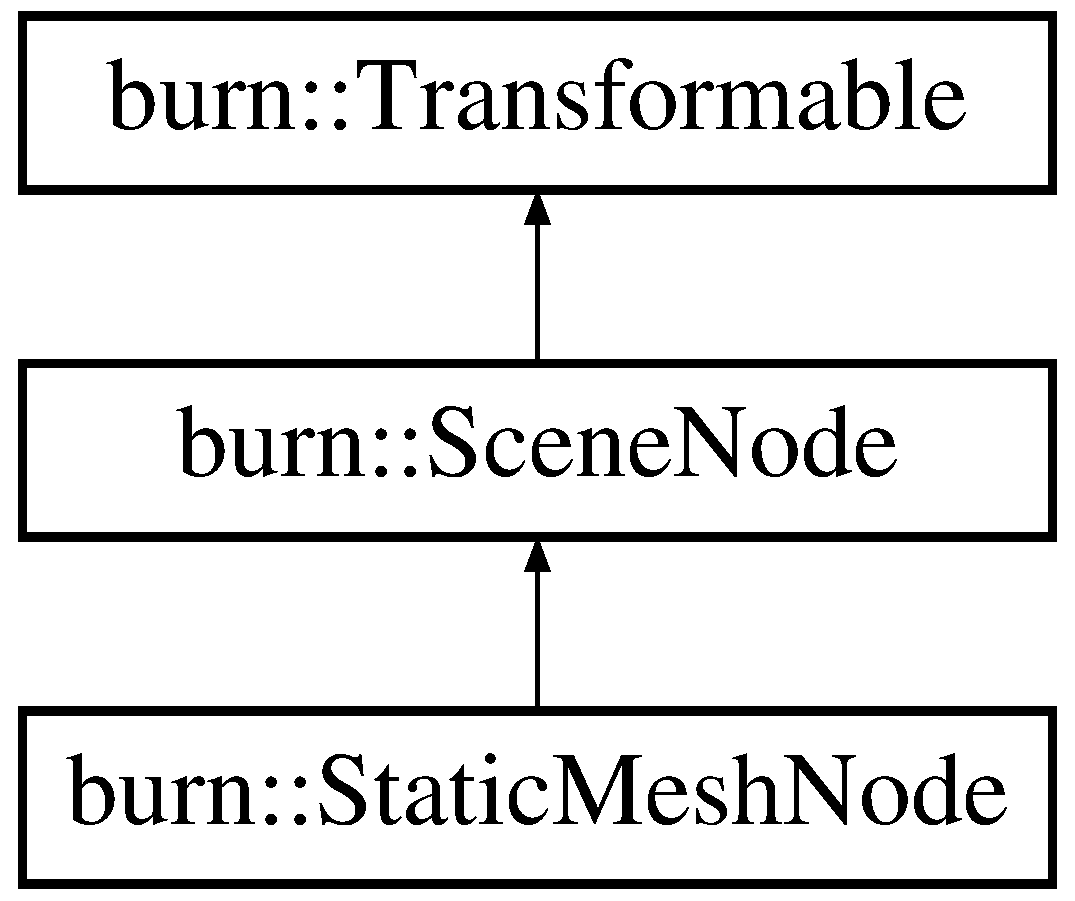
\includegraphics[height=3.000000cm]{classburn_1_1_scene_node}
\end{center}
\end{figure}
\subsection*{Public Member Functions}
\begin{DoxyCompactItemize}
\item 
\hyperlink{classburn_1_1_scene_node_a107d42062677132d1104391fd2bf2530}{Scene\-Node} ()
\begin{DoxyCompactList}\small\item\em Default Constructor. \end{DoxyCompactList}\item 
virtual \hyperlink{classburn_1_1_scene_node_aa651409167ec065930115c8b31057e35}{$\sim$\-Scene\-Node} ()
\begin{DoxyCompactList}\small\item\em Default Destructor. \end{DoxyCompactList}\item 
virtual void \hyperlink{classburn_1_1_scene_node_adcea597571e59f15421c7a9ae0bfdbc3}{draw} (\hyperlink{classburn_1_1_camera}{Camera} $\ast$camera=nullptr)=0
\begin{DoxyCompactList}\small\item\em Virtual method for rendering. \end{DoxyCompactList}\item 
const \hyperlink{classburn_1_1_material}{Material} \& \hyperlink{classburn_1_1_scene_node_a90bbe26a50c9039986bb60b52fd82a7d}{get\-Material} () const 
\begin{DoxyCompactList}\small\item\em Returns the material that the node is using. \end{DoxyCompactList}\item 
void \hyperlink{classburn_1_1_scene_node_a66ab4afa17f078a3814d4bbd88ed9ea1}{set\-Material} (const \hyperlink{classburn_1_1_material}{Material} \&material)
\begin{DoxyCompactList}\small\item\em Sets the material of the node. Influences the rendering behaviour. \end{DoxyCompactList}\end{DoxyCompactItemize}
\subsection*{Protected Attributes}
\begin{DoxyCompactItemize}
\item 
\hyperlink{classburn_1_1_material}{Material} \hyperlink{classburn_1_1_scene_node_a8474c310dafc48e860ebb5ed7ecc7f8f}{\-\_\-material}
\end{DoxyCompactItemize}


\subsection{Constructor \& Destructor Documentation}
\hypertarget{classburn_1_1_scene_node_a107d42062677132d1104391fd2bf2530}{\index{burn\-::\-Scene\-Node@{burn\-::\-Scene\-Node}!Scene\-Node@{Scene\-Node}}
\index{Scene\-Node@{Scene\-Node}!burn::SceneNode@{burn\-::\-Scene\-Node}}
\subsubsection[{Scene\-Node}]{\setlength{\rightskip}{0pt plus 5cm}burn\-::\-Scene\-Node\-::\-Scene\-Node (
\begin{DoxyParamCaption}
{}
\end{DoxyParamCaption}
)}}\label{classburn_1_1_scene_node_a107d42062677132d1104391fd2bf2530}


Default Constructor. 

\hypertarget{classburn_1_1_scene_node_aa651409167ec065930115c8b31057e35}{\index{burn\-::\-Scene\-Node@{burn\-::\-Scene\-Node}!$\sim$\-Scene\-Node@{$\sim$\-Scene\-Node}}
\index{$\sim$\-Scene\-Node@{$\sim$\-Scene\-Node}!burn::SceneNode@{burn\-::\-Scene\-Node}}
\subsubsection[{$\sim$\-Scene\-Node}]{\setlength{\rightskip}{0pt plus 5cm}burn\-::\-Scene\-Node\-::$\sim$\-Scene\-Node (
\begin{DoxyParamCaption}
{}
\end{DoxyParamCaption}
)\hspace{0.3cm}{\ttfamily [virtual]}}}\label{classburn_1_1_scene_node_aa651409167ec065930115c8b31057e35}


Default Destructor. 



\subsection{Member Function Documentation}
\hypertarget{classburn_1_1_scene_node_adcea597571e59f15421c7a9ae0bfdbc3}{\index{burn\-::\-Scene\-Node@{burn\-::\-Scene\-Node}!draw@{draw}}
\index{draw@{draw}!burn::SceneNode@{burn\-::\-Scene\-Node}}
\subsubsection[{draw}]{\setlength{\rightskip}{0pt plus 5cm}virtual void burn\-::\-Scene\-Node\-::draw (
\begin{DoxyParamCaption}
\item[{{\bf Camera} $\ast$}]{camera = {\ttfamily nullptr}}
\end{DoxyParamCaption}
)\hspace{0.3cm}{\ttfamily [pure virtual]}}}\label{classburn_1_1_scene_node_adcea597571e59f15421c7a9ae0bfdbc3}


Virtual method for rendering. 


\begin{DoxyParams}{Parameters}
{\em camera} & Pointer to \hyperlink{classburn_1_1_camera}{Camera} to draw node correctly or nullptr for default rendermode. \\
\hline
\end{DoxyParams}


Implemented in \hyperlink{classburn_1_1_static_mesh_node_a7ff88bee9757061b0393ae5324e7989b}{burn\-::\-Static\-Mesh\-Node}.

\hypertarget{classburn_1_1_scene_node_a90bbe26a50c9039986bb60b52fd82a7d}{\index{burn\-::\-Scene\-Node@{burn\-::\-Scene\-Node}!get\-Material@{get\-Material}}
\index{get\-Material@{get\-Material}!burn::SceneNode@{burn\-::\-Scene\-Node}}
\subsubsection[{get\-Material}]{\setlength{\rightskip}{0pt plus 5cm}const {\bf Material} \& burn\-::\-Scene\-Node\-::get\-Material (
\begin{DoxyParamCaption}
{}
\end{DoxyParamCaption}
) const}}\label{classburn_1_1_scene_node_a90bbe26a50c9039986bb60b52fd82a7d}


Returns the material that the node is using. 

\begin{DoxyReturn}{Returns}
The \hyperlink{classburn_1_1_material}{Material} of the node.
\end{DoxyReturn}
\begin{DoxySeeAlso}{See Also}
\hyperlink{classburn_1_1_scene_node_a66ab4afa17f078a3814d4bbd88ed9ea1}{set\-Material()} 
\end{DoxySeeAlso}
\hypertarget{classburn_1_1_scene_node_a66ab4afa17f078a3814d4bbd88ed9ea1}{\index{burn\-::\-Scene\-Node@{burn\-::\-Scene\-Node}!set\-Material@{set\-Material}}
\index{set\-Material@{set\-Material}!burn::SceneNode@{burn\-::\-Scene\-Node}}
\subsubsection[{set\-Material}]{\setlength{\rightskip}{0pt plus 5cm}void burn\-::\-Scene\-Node\-::set\-Material (
\begin{DoxyParamCaption}
\item[{const {\bf Material} \&}]{material}
\end{DoxyParamCaption}
)}}\label{classburn_1_1_scene_node_a66ab4afa17f078a3814d4bbd88ed9ea1}


Sets the material of the node. Influences the rendering behaviour. 


\begin{DoxyParams}{Parameters}
{\em material} & The \hyperlink{classburn_1_1_material}{Material} to use.\\
\hline
\end{DoxyParams}
\begin{DoxySeeAlso}{See Also}
\hyperlink{classburn_1_1_scene_node_a90bbe26a50c9039986bb60b52fd82a7d}{get\-Material()} 
\end{DoxySeeAlso}


\subsection{Member Data Documentation}
\hypertarget{classburn_1_1_scene_node_a8474c310dafc48e860ebb5ed7ecc7f8f}{\index{burn\-::\-Scene\-Node@{burn\-::\-Scene\-Node}!\-\_\-material@{\-\_\-material}}
\index{\-\_\-material@{\-\_\-material}!burn::SceneNode@{burn\-::\-Scene\-Node}}
\subsubsection[{\-\_\-material}]{\setlength{\rightskip}{0pt plus 5cm}{\bf Material} burn\-::\-Scene\-Node\-::\-\_\-material\hspace{0.3cm}{\ttfamily [protected]}}}\label{classburn_1_1_scene_node_a8474c310dafc48e860ebb5ed7ecc7f8f}


The documentation for this class was generated from the following files\-:\begin{DoxyCompactItemize}
\item 
include/\-Burngine/\-Graphics/\hyperlink{_scene_node_8h}{Scene\-Node.\-h}\item 
include/\-Burngine/\-Graphics/\hyperlink{_scene_node_8cpp}{Scene\-Node.\-cpp}\end{DoxyCompactItemize}

\hypertarget{classburn_1_1_shader}{\section{burn\-:\-:Shader Class Reference}
\label{classburn_1_1_shader}\index{burn\-::\-Shader@{burn\-::\-Shader}}
}


{\ttfamily \#include $<$Shader.\-h$>$}

\subsection*{Public Member Functions}
\begin{DoxyCompactItemize}
\item 
\hyperlink{classburn_1_1_shader_a9795869452f44ff05a2a4b1f278bc990}{Shader} ()
\begin{DoxyCompactList}\small\item\em Default constructor. Default values\-: \end{DoxyCompactList}\item 
\hyperlink{classburn_1_1_shader_a4f67c0a15b6cf9146869cfbcdbdfb541}{$\sim$\-Shader} ()
\begin{DoxyCompactList}\small\item\em Default destructor. Deletes shaderprogram from Open\-G\-L if needed. \end{DoxyCompactList}\item 
bool \hyperlink{classburn_1_1_shader_ae2975b4b68d38d8aa3d045df082e7c2a}{load\-From\-String} (const std\-::string \&vertex\-Shader, const std\-::string \&fragment\-Shader)
\begin{DoxyCompactList}\small\item\em Loads and creates shaderprograms by passing in a vertex-\/ and fragmentshader. \end{DoxyCompactList}\item 
void \hyperlink{classburn_1_1_shader_a8f476e17b38b96d84ea57c31d7aab78d}{activate} () const 
\begin{DoxyCompactList}\small\item\em Activates the shader. It will be used for rendering until no other \hyperlink{classburn_1_1_shader}{Shader} had been called or this one had been destroyed. \end{DoxyCompactList}\item 
G\-Luint \hyperlink{classburn_1_1_shader_ae96b86c6da489d759bec9be7664040dc}{get\-Uniform\-Location} (const std\-::string \&uniform\-Name) const 
\begin{DoxyCompactList}\small\item\em Returns the position of a uniform inside the shaderprogram. This is useful to pass matrices for example. Internal usage mostly. \end{DoxyCompactList}\end{DoxyCompactItemize}


\subsection{Constructor \& Destructor Documentation}
\hypertarget{classburn_1_1_shader_a9795869452f44ff05a2a4b1f278bc990}{\index{burn\-::\-Shader@{burn\-::\-Shader}!Shader@{Shader}}
\index{Shader@{Shader}!burn::Shader@{burn\-::\-Shader}}
\subsubsection[{Shader}]{\setlength{\rightskip}{0pt plus 5cm}burn\-::\-Shader\-::\-Shader (
\begin{DoxyParamCaption}
{}
\end{DoxyParamCaption}
)}}\label{classburn_1_1_shader_a9795869452f44ff05a2a4b1f278bc990}


Default constructor. Default values\-: 


\begin{DoxyItemize}
\item I\-D\-: 0 (invalid I\-D) 
\end{DoxyItemize}\hypertarget{classburn_1_1_shader_a4f67c0a15b6cf9146869cfbcdbdfb541}{\index{burn\-::\-Shader@{burn\-::\-Shader}!$\sim$\-Shader@{$\sim$\-Shader}}
\index{$\sim$\-Shader@{$\sim$\-Shader}!burn::Shader@{burn\-::\-Shader}}
\subsubsection[{$\sim$\-Shader}]{\setlength{\rightskip}{0pt plus 5cm}burn\-::\-Shader\-::$\sim$\-Shader (
\begin{DoxyParamCaption}
{}
\end{DoxyParamCaption}
)}}\label{classburn_1_1_shader_a4f67c0a15b6cf9146869cfbcdbdfb541}


Default destructor. Deletes shaderprogram from Open\-G\-L if needed. 



\subsection{Member Function Documentation}
\hypertarget{classburn_1_1_shader_a8f476e17b38b96d84ea57c31d7aab78d}{\index{burn\-::\-Shader@{burn\-::\-Shader}!activate@{activate}}
\index{activate@{activate}!burn::Shader@{burn\-::\-Shader}}
\subsubsection[{activate}]{\setlength{\rightskip}{0pt plus 5cm}void burn\-::\-Shader\-::activate (
\begin{DoxyParamCaption}
{}
\end{DoxyParamCaption}
) const}}\label{classburn_1_1_shader_a8f476e17b38b96d84ea57c31d7aab78d}


Activates the shader. It will be used for rendering until no other \hyperlink{classburn_1_1_shader}{Shader} had been called or this one had been destroyed. 

\begin{DoxyNote}{Note}
If no \hyperlink{classburn_1_1_shader}{Shader} was created by e.\-g. calling \hyperlink{classburn_1_1_shader_ae2975b4b68d38d8aa3d045df082e7c2a}{load\-From\-String()}, this call will disable shaders at all.
\end{DoxyNote}
\begin{DoxySeeAlso}{See Also}
\hyperlink{classburn_1_1_shader_ae2975b4b68d38d8aa3d045df082e7c2a}{load\-From\-String()} 
\end{DoxySeeAlso}
\hypertarget{classburn_1_1_shader_ae96b86c6da489d759bec9be7664040dc}{\index{burn\-::\-Shader@{burn\-::\-Shader}!get\-Uniform\-Location@{get\-Uniform\-Location}}
\index{get\-Uniform\-Location@{get\-Uniform\-Location}!burn::Shader@{burn\-::\-Shader}}
\subsubsection[{get\-Uniform\-Location}]{\setlength{\rightskip}{0pt plus 5cm}G\-Luint burn\-::\-Shader\-::get\-Uniform\-Location (
\begin{DoxyParamCaption}
\item[{const std\-::string \&}]{uniform\-Name}
\end{DoxyParamCaption}
) const}}\label{classburn_1_1_shader_ae96b86c6da489d759bec9be7664040dc}


Returns the position of a uniform inside the shaderprogram. This is useful to pass matrices for example. Internal usage mostly. 


\begin{DoxyParams}{Parameters}
{\em uniform\-Name} & The name of the uniform.\\
\hline
\end{DoxyParams}
\begin{DoxyReturn}{Returns}
Returns a value $>$= 0 on success or -\/1 when the uniform could not be found. 
\end{DoxyReturn}
\hypertarget{classburn_1_1_shader_ae2975b4b68d38d8aa3d045df082e7c2a}{\index{burn\-::\-Shader@{burn\-::\-Shader}!load\-From\-String@{load\-From\-String}}
\index{load\-From\-String@{load\-From\-String}!burn::Shader@{burn\-::\-Shader}}
\subsubsection[{load\-From\-String}]{\setlength{\rightskip}{0pt plus 5cm}bool burn\-::\-Shader\-::load\-From\-String (
\begin{DoxyParamCaption}
\item[{const std\-::string \&}]{vertex\-Shader, }
\item[{const std\-::string \&}]{fragment\-Shader}
\end{DoxyParamCaption}
)}}\label{classburn_1_1_shader_ae2975b4b68d38d8aa3d045df082e7c2a}


Loads and creates shaderprograms by passing in a vertex-\/ and fragmentshader. 


\begin{DoxyParams}{Parameters}
{\em vertex\-Shader} & The vertexshader. \\
\hline
{\em fragment\-Shader} & The fragmentshader.\\
\hline
\end{DoxyParams}
\begin{DoxyReturn}{Returns}
Returns true when shader was created successfully.
\end{DoxyReturn}
\begin{DoxySeeAlso}{See Also}
\hyperlink{classburn_1_1_shader_a8f476e17b38b96d84ea57c31d7aab78d}{activate()} 
\end{DoxySeeAlso}


The documentation for this class was generated from the following files\-:\begin{DoxyCompactItemize}
\item 
include/\-Burngine/\-Graphics/\hyperlink{_shader_8h}{Shader.\-h}\item 
include/\-Burngine/\-Graphics/\hyperlink{_shader_8cpp}{Shader.\-cpp}\end{DoxyCompactItemize}

\hypertarget{classburn_1_1_static_mesh_node}{\section{burn\-:\-:Static\-Mesh\-Node Class Reference}
\label{classburn_1_1_static_mesh_node}\index{burn\-::\-Static\-Mesh\-Node@{burn\-::\-Static\-Mesh\-Node}}
}


{\ttfamily \#include $<$Static\-Mesh\-Node.\-h$>$}

Inheritance diagram for burn\-:\-:Static\-Mesh\-Node\-:\begin{figure}[H]
\begin{center}
\leavevmode
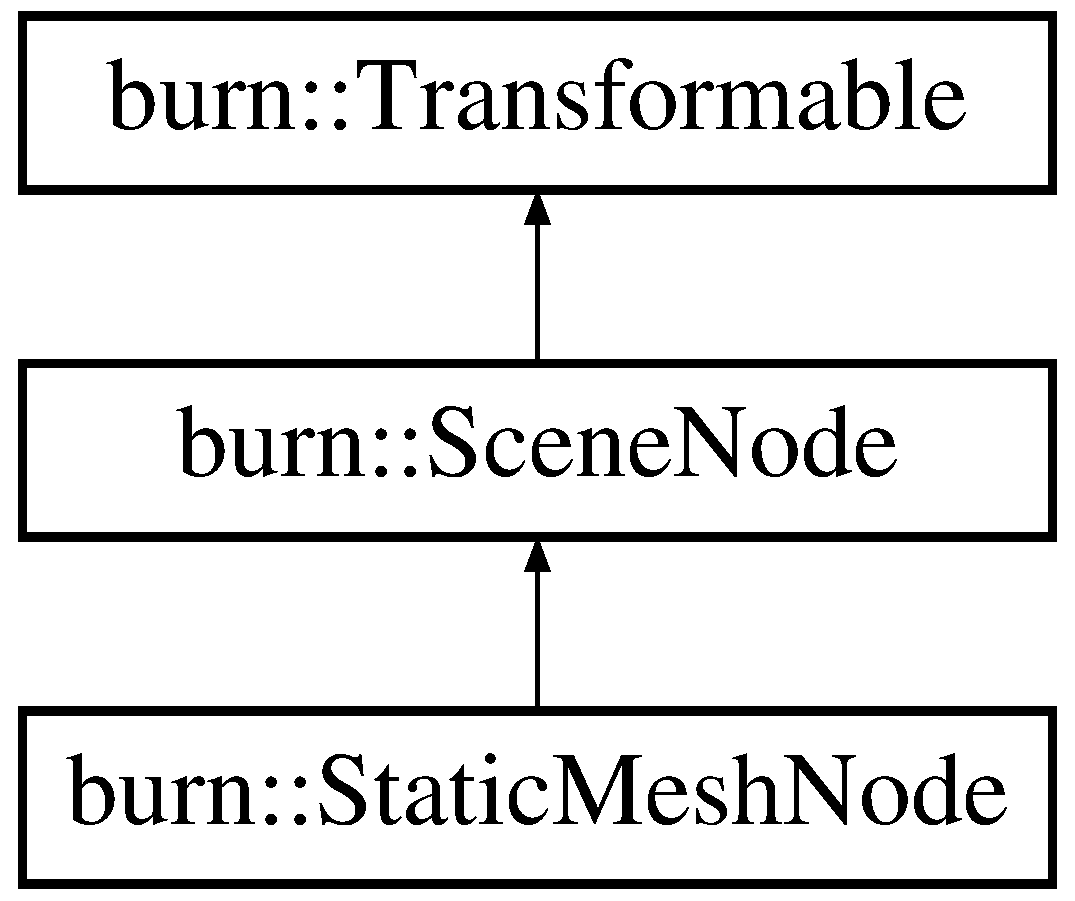
\includegraphics[height=3.000000cm]{classburn_1_1_static_mesh_node}
\end{center}
\end{figure}
\subsection*{Public Member Functions}
\begin{DoxyCompactItemize}
\item 
\hyperlink{classburn_1_1_static_mesh_node_a051ef5fe091cf8e93cc4dd1bae753cbd}{Static\-Mesh\-Node} ()
\item 
\hyperlink{classburn_1_1_static_mesh_node_a68e00b329768da175ee153c46069364e}{$\sim$\-Static\-Mesh\-Node} ()
\item 
void \hyperlink{classburn_1_1_static_mesh_node_af78ecebdfd7c25997caf35ef4ebecdfb}{set\-Mesh} (const \hyperlink{classburn_1_1_mesh}{Mesh} \&mesh)
\item 
const \hyperlink{classburn_1_1_mesh}{Mesh} \& \hyperlink{classburn_1_1_static_mesh_node_ad269a91df547f3a3092d193e4210e081}{get\-Mesh} () const 
\item 
virtual void \hyperlink{classburn_1_1_static_mesh_node_a7ff88bee9757061b0393ae5324e7989b}{draw} (\hyperlink{classburn_1_1_camera}{Camera} $\ast$cam=nullptr)
\end{DoxyCompactItemize}
\subsection*{Additional Inherited Members}


\subsection{Constructor \& Destructor Documentation}
\hypertarget{classburn_1_1_static_mesh_node_a051ef5fe091cf8e93cc4dd1bae753cbd}{\index{burn\-::\-Static\-Mesh\-Node@{burn\-::\-Static\-Mesh\-Node}!Static\-Mesh\-Node@{Static\-Mesh\-Node}}
\index{Static\-Mesh\-Node@{Static\-Mesh\-Node}!burn::StaticMeshNode@{burn\-::\-Static\-Mesh\-Node}}
\subsubsection[{Static\-Mesh\-Node}]{\setlength{\rightskip}{0pt plus 5cm}burn\-::\-Static\-Mesh\-Node\-::\-Static\-Mesh\-Node (
\begin{DoxyParamCaption}
{}
\end{DoxyParamCaption}
)}}\label{classburn_1_1_static_mesh_node_a051ef5fe091cf8e93cc4dd1bae753cbd}
\hypertarget{classburn_1_1_static_mesh_node_a68e00b329768da175ee153c46069364e}{\index{burn\-::\-Static\-Mesh\-Node@{burn\-::\-Static\-Mesh\-Node}!$\sim$\-Static\-Mesh\-Node@{$\sim$\-Static\-Mesh\-Node}}
\index{$\sim$\-Static\-Mesh\-Node@{$\sim$\-Static\-Mesh\-Node}!burn::StaticMeshNode@{burn\-::\-Static\-Mesh\-Node}}
\subsubsection[{$\sim$\-Static\-Mesh\-Node}]{\setlength{\rightskip}{0pt plus 5cm}burn\-::\-Static\-Mesh\-Node\-::$\sim$\-Static\-Mesh\-Node (
\begin{DoxyParamCaption}
{}
\end{DoxyParamCaption}
)}}\label{classburn_1_1_static_mesh_node_a68e00b329768da175ee153c46069364e}


\subsection{Member Function Documentation}
\hypertarget{classburn_1_1_static_mesh_node_a7ff88bee9757061b0393ae5324e7989b}{\index{burn\-::\-Static\-Mesh\-Node@{burn\-::\-Static\-Mesh\-Node}!draw@{draw}}
\index{draw@{draw}!burn::StaticMeshNode@{burn\-::\-Static\-Mesh\-Node}}
\subsubsection[{draw}]{\setlength{\rightskip}{0pt plus 5cm}void burn\-::\-Static\-Mesh\-Node\-::draw (
\begin{DoxyParamCaption}
\item[{{\bf Camera} $\ast$}]{cam = {\ttfamily nullptr}}
\end{DoxyParamCaption}
)\hspace{0.3cm}{\ttfamily [virtual]}}}\label{classburn_1_1_static_mesh_node_a7ff88bee9757061b0393ae5324e7989b}


Implements \hyperlink{classburn_1_1_scene_node_adcea597571e59f15421c7a9ae0bfdbc3}{burn\-::\-Scene\-Node}.

\hypertarget{classburn_1_1_static_mesh_node_ad269a91df547f3a3092d193e4210e081}{\index{burn\-::\-Static\-Mesh\-Node@{burn\-::\-Static\-Mesh\-Node}!get\-Mesh@{get\-Mesh}}
\index{get\-Mesh@{get\-Mesh}!burn::StaticMeshNode@{burn\-::\-Static\-Mesh\-Node}}
\subsubsection[{get\-Mesh}]{\setlength{\rightskip}{0pt plus 5cm}const {\bf Mesh} \& burn\-::\-Static\-Mesh\-Node\-::get\-Mesh (
\begin{DoxyParamCaption}
{}
\end{DoxyParamCaption}
) const}}\label{classburn_1_1_static_mesh_node_ad269a91df547f3a3092d193e4210e081}
\hypertarget{classburn_1_1_static_mesh_node_af78ecebdfd7c25997caf35ef4ebecdfb}{\index{burn\-::\-Static\-Mesh\-Node@{burn\-::\-Static\-Mesh\-Node}!set\-Mesh@{set\-Mesh}}
\index{set\-Mesh@{set\-Mesh}!burn::StaticMeshNode@{burn\-::\-Static\-Mesh\-Node}}
\subsubsection[{set\-Mesh}]{\setlength{\rightskip}{0pt plus 5cm}void burn\-::\-Static\-Mesh\-Node\-::set\-Mesh (
\begin{DoxyParamCaption}
\item[{const {\bf Mesh} \&}]{mesh}
\end{DoxyParamCaption}
)}}\label{classburn_1_1_static_mesh_node_af78ecebdfd7c25997caf35ef4ebecdfb}


The documentation for this class was generated from the following files\-:\begin{DoxyCompactItemize}
\item 
include/\-Burngine/\-Graphics/\hyperlink{_static_mesh_node_8h}{Static\-Mesh\-Node.\-h}\item 
include/\-Burngine/\-Graphics/\hyperlink{_static_mesh_node_8cpp}{Static\-Mesh\-Node.\-cpp}\end{DoxyCompactItemize}

\hypertarget{classburn_1_1_transformable}{\section{burn\-:\-:Transformable Class Reference}
\label{classburn_1_1_transformable}\index{burn\-::\-Transformable@{burn\-::\-Transformable}}
}


Provides methods to move an object in 3\-D-\/space.  




{\ttfamily \#include $<$Transformable.\-h$>$}

Inheritance diagram for burn\-:\-:Transformable\-:\begin{figure}[H]
\begin{center}
\leavevmode
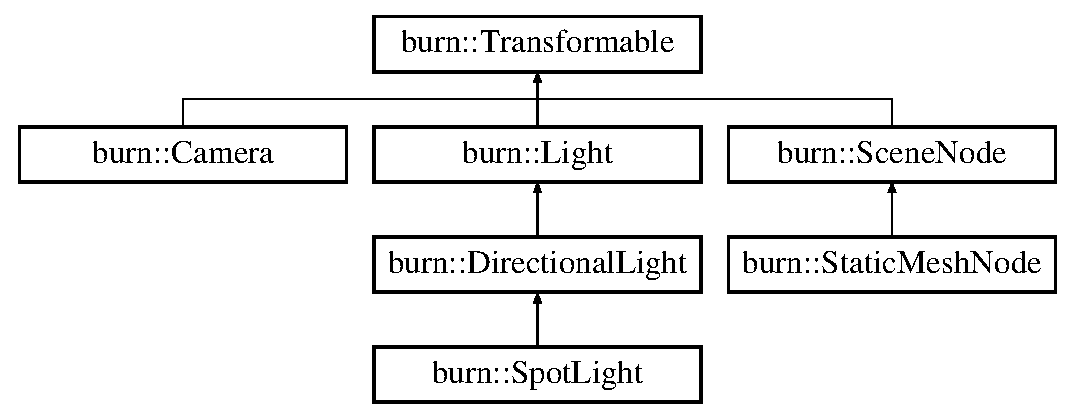
\includegraphics[height=4.000000cm]{classburn_1_1_transformable}
\end{center}
\end{figure}
\subsection*{Public Member Functions}
\begin{DoxyCompactItemize}
\item 
\hyperlink{classburn_1_1_transformable_ab5df8f6f319ebc8888465632a1567981}{Transformable} ()
\begin{DoxyCompactList}\small\item\em The default constructor. \end{DoxyCompactList}\item 
\hyperlink{classburn_1_1_transformable_a96fb19be22efcefb4723781146de28fe}{Transformable} (const \hyperlink{classburn_1_1_transformable}{Transformable} \&other)
\item 
\hyperlink{classburn_1_1_transformable}{Transformable} \& \hyperlink{classburn_1_1_transformable_aee23249ee60e4a3e590046e633c3a979}{operator=} (const \hyperlink{classburn_1_1_transformable}{Transformable} \&other)
\item 
virtual \hyperlink{classburn_1_1_transformable_ac3b6e91f17a6b8f5db8027e72942f269}{$\sim$\-Transformable} ()
\begin{DoxyCompactList}\small\item\em Virtual destructor, because this class should be derived only. \end{DoxyCompactList}\item 
void \hyperlink{classburn_1_1_transformable_a408d484d0ed48c1d7499391b3f2d4a66}{set\-Position} (const \hyperlink{namespaceburn_afdd7cfb352b9612432faf6947b6fff74}{Vector3f} \&position)
\begin{DoxyCompactList}\small\item\em Sets the position of the object. \end{DoxyCompactList}\item 
const \hyperlink{namespaceburn_afdd7cfb352b9612432faf6947b6fff74}{Vector3f} \& \hyperlink{classburn_1_1_transformable_aab2eb6fb8e64349a9f83bc6939477b74}{get\-Position} () const 
\begin{DoxyCompactList}\small\item\em Returns the current position of the object. \end{DoxyCompactList}\item 
void \hyperlink{classburn_1_1_transformable_adad877d654e3ac20ed0ff6edf002e040}{set\-Rotation} (const \hyperlink{namespaceburn_afdd7cfb352b9612432faf6947b6fff74}{Vector3f} \&rotation)
\begin{DoxyCompactList}\small\item\em Sets the rotation of the object. \end{DoxyCompactList}\item 
const \hyperlink{namespaceburn_afdd7cfb352b9612432faf6947b6fff74}{Vector3f} \& \hyperlink{classburn_1_1_transformable_af16b32fb2143e7a459b8446e898c4359}{get\-Rotation} () const 
\begin{DoxyCompactList}\small\item\em Returns the current rotation of the object. \end{DoxyCompactList}\item 
void \hyperlink{classburn_1_1_transformable_a7e73a5706524923d4fc6c13990b7f575}{set\-Scale} (const \hyperlink{namespaceburn_afdd7cfb352b9612432faf6947b6fff74}{Vector3f} \&scale)
\begin{DoxyCompactList}\small\item\em Sets the scale of the object. \end{DoxyCompactList}\item 
const \hyperlink{namespaceburn_afdd7cfb352b9612432faf6947b6fff74}{Vector3f} \& \hyperlink{classburn_1_1_transformable_a62d533b4a7d03b3b2aa9c783cb7cb061}{get\-Scale} () const 
\begin{DoxyCompactList}\small\item\em Return the current scale of the object. \end{DoxyCompactList}\item 
const \hyperlink{namespaceburn_a643e9d2ffceb4304e3755a100268a7a3}{Matrix4f} \& \hyperlink{classburn_1_1_transformable_ac77cb89c24baf4eaf730b478b2f9b2b5}{get\-Model\-Matrix} ()
\begin{DoxyCompactList}\small\item\em Returns the current modelmatrix of the object. \end{DoxyCompactList}\end{DoxyCompactItemize}
\subsection*{Protected Attributes}
\begin{DoxyCompactItemize}
\item 
\hyperlink{namespaceburn_afdd7cfb352b9612432faf6947b6fff74}{Vector3f} \hyperlink{classburn_1_1_transformable_a1cb1a52f8518c7c2f50e45d8cd902767}{\-\_\-position}
\item 
\hyperlink{namespaceburn_afdd7cfb352b9612432faf6947b6fff74}{Vector3f} \hyperlink{classburn_1_1_transformable_a80e5ca4d02b2d58593b751b040e86492}{\-\_\-scale}
\item 
\hyperlink{namespaceburn_afdd7cfb352b9612432faf6947b6fff74}{Vector3f} \hyperlink{classburn_1_1_transformable_ad62e417f44d78cbeedfd30e62c1b896d}{\-\_\-rotation}
\item 
\hyperlink{namespaceburn_a643e9d2ffceb4304e3755a100268a7a3}{Matrix4f} \hyperlink{classburn_1_1_transformable_a6a06bcec86a7f2e70eba6fe7e8bbe61c}{\-\_\-model\-Matrix}
\end{DoxyCompactItemize}


\subsection{Detailed Description}
Provides methods to move an object in 3\-D-\/space. 

\subsection{Constructor \& Destructor Documentation}
\hypertarget{classburn_1_1_transformable_ab5df8f6f319ebc8888465632a1567981}{\index{burn\-::\-Transformable@{burn\-::\-Transformable}!Transformable@{Transformable}}
\index{Transformable@{Transformable}!burn::Transformable@{burn\-::\-Transformable}}
\subsubsection[{Transformable}]{\setlength{\rightskip}{0pt plus 5cm}burn\-::\-Transformable\-::\-Transformable (
\begin{DoxyParamCaption}
{}
\end{DoxyParamCaption}
)}}\label{classburn_1_1_transformable_ab5df8f6f319ebc8888465632a1567981}


The default constructor. 

\hypertarget{classburn_1_1_transformable_a96fb19be22efcefb4723781146de28fe}{\index{burn\-::\-Transformable@{burn\-::\-Transformable}!Transformable@{Transformable}}
\index{Transformable@{Transformable}!burn::Transformable@{burn\-::\-Transformable}}
\subsubsection[{Transformable}]{\setlength{\rightskip}{0pt plus 5cm}burn\-::\-Transformable\-::\-Transformable (
\begin{DoxyParamCaption}
\item[{const {\bf Transformable} \&}]{other}
\end{DoxyParamCaption}
)}}\label{classburn_1_1_transformable_a96fb19be22efcefb4723781146de28fe}
\hypertarget{classburn_1_1_transformable_ac3b6e91f17a6b8f5db8027e72942f269}{\index{burn\-::\-Transformable@{burn\-::\-Transformable}!$\sim$\-Transformable@{$\sim$\-Transformable}}
\index{$\sim$\-Transformable@{$\sim$\-Transformable}!burn::Transformable@{burn\-::\-Transformable}}
\subsubsection[{$\sim$\-Transformable}]{\setlength{\rightskip}{0pt plus 5cm}virtual burn\-::\-Transformable\-::$\sim$\-Transformable (
\begin{DoxyParamCaption}
{}
\end{DoxyParamCaption}
)\hspace{0.3cm}{\ttfamily [virtual]}}}\label{classburn_1_1_transformable_ac3b6e91f17a6b8f5db8027e72942f269}


Virtual destructor, because this class should be derived only. 



\subsection{Member Function Documentation}
\hypertarget{classburn_1_1_transformable_ac77cb89c24baf4eaf730b478b2f9b2b5}{\index{burn\-::\-Transformable@{burn\-::\-Transformable}!get\-Model\-Matrix@{get\-Model\-Matrix}}
\index{get\-Model\-Matrix@{get\-Model\-Matrix}!burn::Transformable@{burn\-::\-Transformable}}
\subsubsection[{get\-Model\-Matrix}]{\setlength{\rightskip}{0pt plus 5cm}const {\bf Matrix4f}\& burn\-::\-Transformable\-::get\-Model\-Matrix (
\begin{DoxyParamCaption}
{}
\end{DoxyParamCaption}
)}}\label{classburn_1_1_transformable_ac77cb89c24baf4eaf730b478b2f9b2b5}


Returns the current modelmatrix of the object. 

\begin{DoxyReturn}{Returns}
The current modelmatrix 
\end{DoxyReturn}
\hypertarget{classburn_1_1_transformable_aab2eb6fb8e64349a9f83bc6939477b74}{\index{burn\-::\-Transformable@{burn\-::\-Transformable}!get\-Position@{get\-Position}}
\index{get\-Position@{get\-Position}!burn::Transformable@{burn\-::\-Transformable}}
\subsubsection[{get\-Position}]{\setlength{\rightskip}{0pt plus 5cm}const {\bf Vector3f}\& burn\-::\-Transformable\-::get\-Position (
\begin{DoxyParamCaption}
{}
\end{DoxyParamCaption}
) const}}\label{classburn_1_1_transformable_aab2eb6fb8e64349a9f83bc6939477b74}


Returns the current position of the object. 

\begin{DoxyReturn}{Returns}
The current position
\end{DoxyReturn}
\begin{DoxySeeAlso}{See Also}
\hyperlink{classburn_1_1_transformable_a408d484d0ed48c1d7499391b3f2d4a66}{set\-Position()} 
\end{DoxySeeAlso}
\hypertarget{classburn_1_1_transformable_af16b32fb2143e7a459b8446e898c4359}{\index{burn\-::\-Transformable@{burn\-::\-Transformable}!get\-Rotation@{get\-Rotation}}
\index{get\-Rotation@{get\-Rotation}!burn::Transformable@{burn\-::\-Transformable}}
\subsubsection[{get\-Rotation}]{\setlength{\rightskip}{0pt plus 5cm}const {\bf Vector3f}\& burn\-::\-Transformable\-::get\-Rotation (
\begin{DoxyParamCaption}
{}
\end{DoxyParamCaption}
) const}}\label{classburn_1_1_transformable_af16b32fb2143e7a459b8446e898c4359}


Returns the current rotation of the object. 

\begin{DoxyReturn}{Returns}
The current rotation
\end{DoxyReturn}
\begin{DoxySeeAlso}{See Also}
\hyperlink{classburn_1_1_transformable_adad877d654e3ac20ed0ff6edf002e040}{set\-Rotation()} 
\end{DoxySeeAlso}
\hypertarget{classburn_1_1_transformable_a62d533b4a7d03b3b2aa9c783cb7cb061}{\index{burn\-::\-Transformable@{burn\-::\-Transformable}!get\-Scale@{get\-Scale}}
\index{get\-Scale@{get\-Scale}!burn::Transformable@{burn\-::\-Transformable}}
\subsubsection[{get\-Scale}]{\setlength{\rightskip}{0pt plus 5cm}const {\bf Vector3f}\& burn\-::\-Transformable\-::get\-Scale (
\begin{DoxyParamCaption}
{}
\end{DoxyParamCaption}
) const}}\label{classburn_1_1_transformable_a62d533b4a7d03b3b2aa9c783cb7cb061}


Return the current scale of the object. 

\begin{DoxyReturn}{Returns}
The current scale
\end{DoxyReturn}
\begin{DoxySeeAlso}{See Also}
\hyperlink{classburn_1_1_transformable_a7e73a5706524923d4fc6c13990b7f575}{set\-Scale()} 
\end{DoxySeeAlso}
\hypertarget{classburn_1_1_transformable_aee23249ee60e4a3e590046e633c3a979}{\index{burn\-::\-Transformable@{burn\-::\-Transformable}!operator=@{operator=}}
\index{operator=@{operator=}!burn::Transformable@{burn\-::\-Transformable}}
\subsubsection[{operator=}]{\setlength{\rightskip}{0pt plus 5cm}{\bf Transformable}\& burn\-::\-Transformable\-::operator= (
\begin{DoxyParamCaption}
\item[{const {\bf Transformable} \&}]{other}
\end{DoxyParamCaption}
)}}\label{classburn_1_1_transformable_aee23249ee60e4a3e590046e633c3a979}
\hypertarget{classburn_1_1_transformable_a408d484d0ed48c1d7499391b3f2d4a66}{\index{burn\-::\-Transformable@{burn\-::\-Transformable}!set\-Position@{set\-Position}}
\index{set\-Position@{set\-Position}!burn::Transformable@{burn\-::\-Transformable}}
\subsubsection[{set\-Position}]{\setlength{\rightskip}{0pt plus 5cm}void burn\-::\-Transformable\-::set\-Position (
\begin{DoxyParamCaption}
\item[{const {\bf Vector3f} \&}]{position}
\end{DoxyParamCaption}
)}}\label{classburn_1_1_transformable_a408d484d0ed48c1d7499391b3f2d4a66}


Sets the position of the object. 


\begin{DoxyParams}{Parameters}
{\em position} & The new position\\
\hline
\end{DoxyParams}
\begin{DoxySeeAlso}{See Also}
\hyperlink{classburn_1_1_transformable_aab2eb6fb8e64349a9f83bc6939477b74}{get\-Position()} 
\end{DoxySeeAlso}
\hypertarget{classburn_1_1_transformable_adad877d654e3ac20ed0ff6edf002e040}{\index{burn\-::\-Transformable@{burn\-::\-Transformable}!set\-Rotation@{set\-Rotation}}
\index{set\-Rotation@{set\-Rotation}!burn::Transformable@{burn\-::\-Transformable}}
\subsubsection[{set\-Rotation}]{\setlength{\rightskip}{0pt plus 5cm}void burn\-::\-Transformable\-::set\-Rotation (
\begin{DoxyParamCaption}
\item[{const {\bf Vector3f} \&}]{rotation}
\end{DoxyParamCaption}
)}}\label{classburn_1_1_transformable_adad877d654e3ac20ed0ff6edf002e040}


Sets the rotation of the object. 


\begin{DoxyParams}{Parameters}
{\em rotation} & The new rotation\\
\hline
\end{DoxyParams}
\begin{DoxySeeAlso}{See Also}
\hyperlink{classburn_1_1_transformable_af16b32fb2143e7a459b8446e898c4359}{get\-Rotation()} 
\end{DoxySeeAlso}
\hypertarget{classburn_1_1_transformable_a7e73a5706524923d4fc6c13990b7f575}{\index{burn\-::\-Transformable@{burn\-::\-Transformable}!set\-Scale@{set\-Scale}}
\index{set\-Scale@{set\-Scale}!burn::Transformable@{burn\-::\-Transformable}}
\subsubsection[{set\-Scale}]{\setlength{\rightskip}{0pt plus 5cm}void burn\-::\-Transformable\-::set\-Scale (
\begin{DoxyParamCaption}
\item[{const {\bf Vector3f} \&}]{scale}
\end{DoxyParamCaption}
)}}\label{classburn_1_1_transformable_a7e73a5706524923d4fc6c13990b7f575}


Sets the scale of the object. 


\begin{DoxyParams}{Parameters}
{\em scale} & The new scale\\
\hline
\end{DoxyParams}
\begin{DoxySeeAlso}{See Also}
\hyperlink{classburn_1_1_transformable_a62d533b4a7d03b3b2aa9c783cb7cb061}{get\-Scale()} 
\end{DoxySeeAlso}


\subsection{Member Data Documentation}
\hypertarget{classburn_1_1_transformable_a6a06bcec86a7f2e70eba6fe7e8bbe61c}{\index{burn\-::\-Transformable@{burn\-::\-Transformable}!\-\_\-model\-Matrix@{\-\_\-model\-Matrix}}
\index{\-\_\-model\-Matrix@{\-\_\-model\-Matrix}!burn::Transformable@{burn\-::\-Transformable}}
\subsubsection[{\-\_\-model\-Matrix}]{\setlength{\rightskip}{0pt plus 5cm}{\bf Matrix4f} burn\-::\-Transformable\-::\-\_\-model\-Matrix\hspace{0.3cm}{\ttfamily [protected]}}}\label{classburn_1_1_transformable_a6a06bcec86a7f2e70eba6fe7e8bbe61c}
\hypertarget{classburn_1_1_transformable_a1cb1a52f8518c7c2f50e45d8cd902767}{\index{burn\-::\-Transformable@{burn\-::\-Transformable}!\-\_\-position@{\-\_\-position}}
\index{\-\_\-position@{\-\_\-position}!burn::Transformable@{burn\-::\-Transformable}}
\subsubsection[{\-\_\-position}]{\setlength{\rightskip}{0pt plus 5cm}{\bf Vector3f} burn\-::\-Transformable\-::\-\_\-position\hspace{0.3cm}{\ttfamily [protected]}}}\label{classburn_1_1_transformable_a1cb1a52f8518c7c2f50e45d8cd902767}
\hypertarget{classburn_1_1_transformable_ad62e417f44d78cbeedfd30e62c1b896d}{\index{burn\-::\-Transformable@{burn\-::\-Transformable}!\-\_\-rotation@{\-\_\-rotation}}
\index{\-\_\-rotation@{\-\_\-rotation}!burn::Transformable@{burn\-::\-Transformable}}
\subsubsection[{\-\_\-rotation}]{\setlength{\rightskip}{0pt plus 5cm}{\bf Vector3f} burn\-::\-Transformable\-::\-\_\-rotation\hspace{0.3cm}{\ttfamily [protected]}}}\label{classburn_1_1_transformable_ad62e417f44d78cbeedfd30e62c1b896d}
\hypertarget{classburn_1_1_transformable_a80e5ca4d02b2d58593b751b040e86492}{\index{burn\-::\-Transformable@{burn\-::\-Transformable}!\-\_\-scale@{\-\_\-scale}}
\index{\-\_\-scale@{\-\_\-scale}!burn::Transformable@{burn\-::\-Transformable}}
\subsubsection[{\-\_\-scale}]{\setlength{\rightskip}{0pt plus 5cm}{\bf Vector3f} burn\-::\-Transformable\-::\-\_\-scale\hspace{0.3cm}{\ttfamily [protected]}}}\label{classburn_1_1_transformable_a80e5ca4d02b2d58593b751b040e86492}


The documentation for this class was generated from the following file\-:\begin{DoxyCompactItemize}
\item 
include/\-Burngine/\-Graphics/\-Scene/\hyperlink{_transformable_8h}{Transformable.\-h}\end{DoxyCompactItemize}

\hypertarget{classburn_1_1_vertex}{\section{burn\-:\-:Vertex Class Reference}
\label{classburn_1_1_vertex}\index{burn\-::\-Vertex@{burn\-::\-Vertex}}
}


{\ttfamily \#include $<$Vertex.\-h$>$}

\subsection*{Public Member Functions}
\begin{DoxyCompactItemize}
\item 
\hyperlink{classburn_1_1_vertex_ae8eacfebc5e61f6660f875fb6eefdb03}{Vertex} (const \hyperlink{namespaceburn_a9d6d349c94bc4dc9699427216128a0ef}{Vector3f} \&position=\hyperlink{namespaceburn_a9d6d349c94bc4dc9699427216128a0ef}{Vector3f}(), const \hyperlink{namespaceburn_a9d6d349c94bc4dc9699427216128a0ef}{Vector3f} \&color=\hyperlink{namespaceburn_a9d6d349c94bc4dc9699427216128a0ef}{Vector3f}(), const \hyperlink{namespaceburn_a2af71ec5609a2f2d501827804e86a9b8}{Vector2f} \&uv=\hyperlink{namespaceburn_a2af71ec5609a2f2d501827804e86a9b8}{Vector2f}())
\item 
\hyperlink{classburn_1_1_vertex_ad950d9459711c1ba4223de35623f75b6}{$\sim$\-Vertex} ()
\item 
void \hyperlink{classburn_1_1_vertex_aa38bae183bbe857f9fabeb8e5510e9a0}{set\-Position} (const \hyperlink{namespaceburn_a9d6d349c94bc4dc9699427216128a0ef}{Vector3f} \&position)
\item 
const \hyperlink{namespaceburn_a9d6d349c94bc4dc9699427216128a0ef}{Vector3f} \& \hyperlink{classburn_1_1_vertex_afdc13277da83f244302ddfc1b6863444}{get\-Position} () const 
\item 
void \hyperlink{classburn_1_1_vertex_a57e2bf8a6e58c7d02c8431f03239cc6b}{set\-Color} (const \hyperlink{namespaceburn_a9d6d349c94bc4dc9699427216128a0ef}{Vector3f} \&color)
\item 
const \hyperlink{namespaceburn_a9d6d349c94bc4dc9699427216128a0ef}{Vector3f} \& \hyperlink{classburn_1_1_vertex_a1dcb11a63a04b0e279e8a69df85dd8d6}{get\-Color} () const 
\item 
void \hyperlink{classburn_1_1_vertex_afc4eff1b4065852cb856b690006e0bd8}{set\-Uv} (const \hyperlink{namespaceburn_a2af71ec5609a2f2d501827804e86a9b8}{Vector2f} \&uv)
\item 
const \hyperlink{namespaceburn_a2af71ec5609a2f2d501827804e86a9b8}{Vector2f} \& \hyperlink{classburn_1_1_vertex_a277e9b082825c211acf730b46580301a}{get\-Uv} () const 
\end{DoxyCompactItemize}


\subsection{Constructor \& Destructor Documentation}
\hypertarget{classburn_1_1_vertex_ae8eacfebc5e61f6660f875fb6eefdb03}{\index{burn\-::\-Vertex@{burn\-::\-Vertex}!Vertex@{Vertex}}
\index{Vertex@{Vertex}!burn::Vertex@{burn\-::\-Vertex}}
\subsubsection[{Vertex}]{\setlength{\rightskip}{0pt plus 5cm}burn\-::\-Vertex\-::\-Vertex (
\begin{DoxyParamCaption}
\item[{const {\bf Vector3f} \&}]{position = {\ttfamily {\bf Vector3f}()}, }
\item[{const {\bf Vector3f} \&}]{color = {\ttfamily {\bf Vector3f}()}, }
\item[{const {\bf Vector2f} \&}]{uv = {\ttfamily {\bf Vector2f}()}}
\end{DoxyParamCaption}
)}}\label{classburn_1_1_vertex_ae8eacfebc5e61f6660f875fb6eefdb03}
\hypertarget{classburn_1_1_vertex_ad950d9459711c1ba4223de35623f75b6}{\index{burn\-::\-Vertex@{burn\-::\-Vertex}!$\sim$\-Vertex@{$\sim$\-Vertex}}
\index{$\sim$\-Vertex@{$\sim$\-Vertex}!burn::Vertex@{burn\-::\-Vertex}}
\subsubsection[{$\sim$\-Vertex}]{\setlength{\rightskip}{0pt plus 5cm}burn\-::\-Vertex\-::$\sim$\-Vertex (
\begin{DoxyParamCaption}
{}
\end{DoxyParamCaption}
)}}\label{classburn_1_1_vertex_ad950d9459711c1ba4223de35623f75b6}


\subsection{Member Function Documentation}
\hypertarget{classburn_1_1_vertex_a1dcb11a63a04b0e279e8a69df85dd8d6}{\index{burn\-::\-Vertex@{burn\-::\-Vertex}!get\-Color@{get\-Color}}
\index{get\-Color@{get\-Color}!burn::Vertex@{burn\-::\-Vertex}}
\subsubsection[{get\-Color}]{\setlength{\rightskip}{0pt plus 5cm}const {\bf Vector3f} \& burn\-::\-Vertex\-::get\-Color (
\begin{DoxyParamCaption}
{}
\end{DoxyParamCaption}
) const}}\label{classburn_1_1_vertex_a1dcb11a63a04b0e279e8a69df85dd8d6}
\hypertarget{classburn_1_1_vertex_afdc13277da83f244302ddfc1b6863444}{\index{burn\-::\-Vertex@{burn\-::\-Vertex}!get\-Position@{get\-Position}}
\index{get\-Position@{get\-Position}!burn::Vertex@{burn\-::\-Vertex}}
\subsubsection[{get\-Position}]{\setlength{\rightskip}{0pt plus 5cm}const {\bf Vector3f} \& burn\-::\-Vertex\-::get\-Position (
\begin{DoxyParamCaption}
{}
\end{DoxyParamCaption}
) const}}\label{classburn_1_1_vertex_afdc13277da83f244302ddfc1b6863444}
\hypertarget{classburn_1_1_vertex_a277e9b082825c211acf730b46580301a}{\index{burn\-::\-Vertex@{burn\-::\-Vertex}!get\-Uv@{get\-Uv}}
\index{get\-Uv@{get\-Uv}!burn::Vertex@{burn\-::\-Vertex}}
\subsubsection[{get\-Uv}]{\setlength{\rightskip}{0pt plus 5cm}const {\bf Vector2f} \& burn\-::\-Vertex\-::get\-Uv (
\begin{DoxyParamCaption}
{}
\end{DoxyParamCaption}
) const}}\label{classburn_1_1_vertex_a277e9b082825c211acf730b46580301a}
\hypertarget{classburn_1_1_vertex_a57e2bf8a6e58c7d02c8431f03239cc6b}{\index{burn\-::\-Vertex@{burn\-::\-Vertex}!set\-Color@{set\-Color}}
\index{set\-Color@{set\-Color}!burn::Vertex@{burn\-::\-Vertex}}
\subsubsection[{set\-Color}]{\setlength{\rightskip}{0pt plus 5cm}void burn\-::\-Vertex\-::set\-Color (
\begin{DoxyParamCaption}
\item[{const {\bf Vector3f} \&}]{color}
\end{DoxyParamCaption}
)}}\label{classburn_1_1_vertex_a57e2bf8a6e58c7d02c8431f03239cc6b}
\hypertarget{classburn_1_1_vertex_aa38bae183bbe857f9fabeb8e5510e9a0}{\index{burn\-::\-Vertex@{burn\-::\-Vertex}!set\-Position@{set\-Position}}
\index{set\-Position@{set\-Position}!burn::Vertex@{burn\-::\-Vertex}}
\subsubsection[{set\-Position}]{\setlength{\rightskip}{0pt plus 5cm}void burn\-::\-Vertex\-::set\-Position (
\begin{DoxyParamCaption}
\item[{const {\bf Vector3f} \&}]{position}
\end{DoxyParamCaption}
)}}\label{classburn_1_1_vertex_aa38bae183bbe857f9fabeb8e5510e9a0}
\hypertarget{classburn_1_1_vertex_afc4eff1b4065852cb856b690006e0bd8}{\index{burn\-::\-Vertex@{burn\-::\-Vertex}!set\-Uv@{set\-Uv}}
\index{set\-Uv@{set\-Uv}!burn::Vertex@{burn\-::\-Vertex}}
\subsubsection[{set\-Uv}]{\setlength{\rightskip}{0pt plus 5cm}void burn\-::\-Vertex\-::set\-Uv (
\begin{DoxyParamCaption}
\item[{const {\bf Vector2f} \&}]{uv}
\end{DoxyParamCaption}
)}}\label{classburn_1_1_vertex_afc4eff1b4065852cb856b690006e0bd8}


The documentation for this class was generated from the following files\-:\begin{DoxyCompactItemize}
\item 
include/\-Burngine/\-Graphics/\hyperlink{_vertex_8h}{Vertex.\-h}\item 
include/\-Burngine/\-Graphics/\hyperlink{_vertex_8cpp}{Vertex.\-cpp}\end{DoxyCompactItemize}

\hypertarget{classburn_1_1_window}{\section{burn\-:\-:Window Class Reference}
\label{classburn_1_1_window}\index{burn\-::\-Window@{burn\-::\-Window}}
}


The most important class of Burngine. It defines the Open\-G\-L-\/\-Context which is needed for all graphical commands.  




{\ttfamily \#include $<$Window.\-h$>$}

\subsection*{Public Types}
\begin{DoxyCompactItemize}
\item 
enum \hyperlink{classburn_1_1_window_ab964403748eb7540e38e649e81711da3}{Blend\-Mode} \{ \hyperlink{classburn_1_1_window_ab964403748eb7540e38e649e81711da3a332b363e82d02455450855da94d4311d}{O\-V\-E\-R\-W\-R\-I\-T\-E}, 
\hyperlink{classburn_1_1_window_ab964403748eb7540e38e649e81711da3acd775a8203f8a3c574eef9858fd3ccb0}{A\-D\-D}, 
\hyperlink{classburn_1_1_window_ab964403748eb7540e38e649e81711da3a012f10a0a89f5327bac712313452f919}{M\-U\-L\-T\-I\-P\-L\-Y}
 \}
\end{DoxyCompactItemize}
\subsection*{Public Member Functions}
\begin{DoxyCompactItemize}
\item 
\hyperlink{classburn_1_1_window_acc7f6464e1ed22854f41342becb51e62}{Window} ()
\begin{DoxyCompactList}\small\item\em The default constructor. \end{DoxyCompactList}\item 
\hyperlink{classburn_1_1_window_a47bd487f48808cab78faa5713e15f0c3}{$\sim$\-Window} ()
\begin{DoxyCompactList}\small\item\em The default destructor. \end{DoxyCompactList}\item 
bool \hyperlink{classburn_1_1_window_a6b8ac2866e1997d479becef84b3a4cf2}{create} (const \hyperlink{classburn_1_1_window_settings}{Window\-Settings} \&ws=\hyperlink{classburn_1_1_window_settings}{Window\-Settings}(), bool load\-Shaders=true)
\begin{DoxyCompactList}\small\item\em Creates a window defined by \hyperlink{classburn_1_1_window_settings}{Window\-Settings}. \end{DoxyCompactList}\item 
const \hyperlink{classburn_1_1_window_settings}{Window\-Settings} \& \hyperlink{classburn_1_1_window_a988e564ed812770ae184cf22bf05e730}{get\-Settings} () const 
\item 
bool \hyperlink{classburn_1_1_window_a1bed3eba8c1da3f0a58a3ed5de2c1071}{close} ()
\begin{DoxyCompactList}\small\item\em Destroys the current window. \end{DoxyCompactList}\item 
bool \hyperlink{classburn_1_1_window_aefd7af7009fee4982b04ac946540f7ee}{keep\-Opened} () const 
\begin{DoxyCompactList}\small\item\em This call will check events which want to close the window. \end{DoxyCompactList}\item 
void \hyperlink{classburn_1_1_window_a81e1da9f111938b38bc4c2c06dac9cfd}{update} ()
\begin{DoxyCompactList}\small\item\em Updates and handles all events. This must be called again and again in order to tell the O\-S that the program is not stuck and running fine. \end{DoxyCompactList}\item 
void \hyperlink{classburn_1_1_window_a2e6c75cedaeb5571aaac2921bf8bcb6e}{clear} () const 
\begin{DoxyCompactList}\small\item\em Cleares the back buffer. (The buffer on which Burngine is rendering) \end{DoxyCompactList}\item 
void \hyperlink{classburn_1_1_window_a017ddbce346ebe3e11e2abc6ce0948e0}{display} ()
\begin{DoxyCompactList}\small\item\em Swaps the back buffer with the front buffer. Due to the call the buffer on which had been drawn will be displayed. \end{DoxyCompactList}\item 
void \hyperlink{classburn_1_1_window_a840d45e13910496fe9edd45d844e46a1}{set\-Framerate\-Limit} (const unsigned int \&fps)
\begin{DoxyCompactList}\small\item\em Caps the framerate of the window. Set 0 (default) to disable the framerate limit. \end{DoxyCompactList}\item 
const unsigned int \& \hyperlink{classburn_1_1_window_aa694b6ed57c02e625fff074f31a107c9}{get\-Framerate\-Limit} () const 
\begin{DoxyCompactList}\small\item\em Returns the current framerate limit of the window. \end{DoxyCompactList}\item 
const double \& \hyperlink{classburn_1_1_window_ae5af78665f468bd19ebb38a8ac13b701}{get\-Elapsed\-Time} () const 
\begin{DoxyCompactList}\small\item\em Returns the time in seconds which was needed to draw the last frame. This is useful to make calculations framerate-\/independing but depending on time. \end{DoxyCompactList}\item 
void \hyperlink{classburn_1_1_window_a7bfc2454c14e5065c67d6bd86cb0af92}{bind} () const 
\item 
std\-::shared\-\_\-ptr$<$ \hyperlink{classburn_1_1_scene}{Scene} $>$ \hyperlink{classburn_1_1_window_acd7968ffd781f6f62259171e4c633031}{create\-Scene} ()
\item 
void \hyperlink{classburn_1_1_window_a4beebeb46f4b35c38c382e1042288f18}{remove\-Scene} (const std\-::shared\-\_\-ptr$<$ \hyperlink{classburn_1_1_scene}{Scene} $>$ \&scene)
\end{DoxyCompactItemize}
\subsection*{Static Public Member Functions}
\begin{DoxyCompactItemize}
\item 
static bool \hyperlink{classburn_1_1_window_ab5f58992b7d89ca04c57516bd128780c}{is\-Context\-Created} ()
\begin{DoxyCompactList}\small\item\em This function is used to ensure, that an Open\-G\-L-\/\-Context exists. Calling Open\-G\-L-\/\-Methods will result in crashes when no context is created. This is internally used by all classes that call Open\-G\-L-\/\-Methods. \end{DoxyCompactList}\item 
static void \hyperlink{classburn_1_1_window_a8398c823ad79ab6c2a300f021ff556b6}{set\-Blend\-Mode} (const \hyperlink{classburn_1_1_window_ab964403748eb7540e38e649e81711da3}{Blend\-Mode} \&blend\-Mode)
\begin{DoxyCompactList}\small\item\em This is used to set the blending mode when rendering. Initially O\-V\-E\-R\-W\-R\-I\-T\-E is used. So everything you draw will ignore, what was already drawn. \end{DoxyCompactList}\end{DoxyCompactItemize}


\subsection{Detailed Description}
The most important class of Burngine. It defines the Open\-G\-L-\/\-Context which is needed for all graphical commands. 

\subsection{Member Enumeration Documentation}
\hypertarget{classburn_1_1_window_ab964403748eb7540e38e649e81711da3}{\index{burn\-::\-Window@{burn\-::\-Window}!Blend\-Mode@{Blend\-Mode}}
\index{Blend\-Mode@{Blend\-Mode}!burn::Window@{burn\-::\-Window}}
\subsubsection[{Blend\-Mode}]{\setlength{\rightskip}{0pt plus 5cm}enum {\bf burn\-::\-Window\-::\-Blend\-Mode}}}\label{classburn_1_1_window_ab964403748eb7540e38e649e81711da3}
\begin{Desc}
\item[Enumerator]\par
\begin{description}
\index{O\-V\-E\-R\-W\-R\-I\-T\-E@{O\-V\-E\-R\-W\-R\-I\-T\-E}!burn\-::\-Window@{burn\-::\-Window}}\index{burn\-::\-Window@{burn\-::\-Window}!O\-V\-E\-R\-W\-R\-I\-T\-E@{O\-V\-E\-R\-W\-R\-I\-T\-E}}\item[{\em 
\hypertarget{classburn_1_1_window_ab964403748eb7540e38e649e81711da3a332b363e82d02455450855da94d4311d}{O\-V\-E\-R\-W\-R\-I\-T\-E}\label{classburn_1_1_window_ab964403748eb7540e38e649e81711da3a332b363e82d02455450855da94d4311d}
}]\index{A\-D\-D@{A\-D\-D}!burn\-::\-Window@{burn\-::\-Window}}\index{burn\-::\-Window@{burn\-::\-Window}!A\-D\-D@{A\-D\-D}}\item[{\em 
\hypertarget{classburn_1_1_window_ab964403748eb7540e38e649e81711da3acd775a8203f8a3c574eef9858fd3ccb0}{A\-D\-D}\label{classburn_1_1_window_ab964403748eb7540e38e649e81711da3acd775a8203f8a3c574eef9858fd3ccb0}
}]\index{M\-U\-L\-T\-I\-P\-L\-Y@{M\-U\-L\-T\-I\-P\-L\-Y}!burn\-::\-Window@{burn\-::\-Window}}\index{burn\-::\-Window@{burn\-::\-Window}!M\-U\-L\-T\-I\-P\-L\-Y@{M\-U\-L\-T\-I\-P\-L\-Y}}\item[{\em 
\hypertarget{classburn_1_1_window_ab964403748eb7540e38e649e81711da3a012f10a0a89f5327bac712313452f919}{M\-U\-L\-T\-I\-P\-L\-Y}\label{classburn_1_1_window_ab964403748eb7540e38e649e81711da3a012f10a0a89f5327bac712313452f919}
}]\end{description}
\end{Desc}


\subsection{Constructor \& Destructor Documentation}
\hypertarget{classburn_1_1_window_acc7f6464e1ed22854f41342becb51e62}{\index{burn\-::\-Window@{burn\-::\-Window}!Window@{Window}}
\index{Window@{Window}!burn::Window@{burn\-::\-Window}}
\subsubsection[{Window}]{\setlength{\rightskip}{0pt plus 5cm}burn\-::\-Window\-::\-Window (
\begin{DoxyParamCaption}
{}
\end{DoxyParamCaption}
)}}\label{classburn_1_1_window_acc7f6464e1ed22854f41342becb51e62}


The default constructor. 

\hypertarget{classburn_1_1_window_a47bd487f48808cab78faa5713e15f0c3}{\index{burn\-::\-Window@{burn\-::\-Window}!$\sim$\-Window@{$\sim$\-Window}}
\index{$\sim$\-Window@{$\sim$\-Window}!burn::Window@{burn\-::\-Window}}
\subsubsection[{$\sim$\-Window}]{\setlength{\rightskip}{0pt plus 5cm}burn\-::\-Window\-::$\sim$\-Window (
\begin{DoxyParamCaption}
{}
\end{DoxyParamCaption}
)}}\label{classburn_1_1_window_a47bd487f48808cab78faa5713e15f0c3}


The default destructor. 



\subsection{Member Function Documentation}
\hypertarget{classburn_1_1_window_a7bfc2454c14e5065c67d6bd86cb0af92}{\index{burn\-::\-Window@{burn\-::\-Window}!bind@{bind}}
\index{bind@{bind}!burn::Window@{burn\-::\-Window}}
\subsubsection[{bind}]{\setlength{\rightskip}{0pt plus 5cm}void burn\-::\-Window\-::bind (
\begin{DoxyParamCaption}
{}
\end{DoxyParamCaption}
) const}}\label{classburn_1_1_window_a7bfc2454c14e5065c67d6bd86cb0af92}
\hypertarget{classburn_1_1_window_a2e6c75cedaeb5571aaac2921bf8bcb6e}{\index{burn\-::\-Window@{burn\-::\-Window}!clear@{clear}}
\index{clear@{clear}!burn::Window@{burn\-::\-Window}}
\subsubsection[{clear}]{\setlength{\rightskip}{0pt plus 5cm}void burn\-::\-Window\-::clear (
\begin{DoxyParamCaption}
{}
\end{DoxyParamCaption}
) const}}\label{classburn_1_1_window_a2e6c75cedaeb5571aaac2921bf8bcb6e}


Cleares the back buffer. (The buffer on which Burngine is rendering) 

\hypertarget{classburn_1_1_window_a1bed3eba8c1da3f0a58a3ed5de2c1071}{\index{burn\-::\-Window@{burn\-::\-Window}!close@{close}}
\index{close@{close}!burn::Window@{burn\-::\-Window}}
\subsubsection[{close}]{\setlength{\rightskip}{0pt plus 5cm}bool burn\-::\-Window\-::close (
\begin{DoxyParamCaption}
{}
\end{DoxyParamCaption}
)}}\label{classburn_1_1_window_a1bed3eba8c1da3f0a58a3ed5de2c1071}


Destroys the current window. 

\begin{DoxyReturn}{Returns}
Returns true on success
\end{DoxyReturn}
\begin{DoxySeeAlso}{See Also}
\hyperlink{classburn_1_1_window_a6b8ac2866e1997d479becef84b3a4cf2}{create()} 
\end{DoxySeeAlso}
\hypertarget{classburn_1_1_window_a6b8ac2866e1997d479becef84b3a4cf2}{\index{burn\-::\-Window@{burn\-::\-Window}!create@{create}}
\index{create@{create}!burn::Window@{burn\-::\-Window}}
\subsubsection[{create}]{\setlength{\rightskip}{0pt plus 5cm}bool burn\-::\-Window\-::create (
\begin{DoxyParamCaption}
\item[{const {\bf Window\-Settings} \&}]{ws = {\ttfamily {\bf Window\-Settings}()}, }
\item[{bool}]{load\-Shaders = {\ttfamily true}}
\end{DoxyParamCaption}
)}}\label{classburn_1_1_window_a6b8ac2866e1997d479becef84b3a4cf2}


Creates a window defined by \hyperlink{classburn_1_1_window_settings}{Window\-Settings}. 


\begin{DoxyParams}{Parameters}
{\em ws} & The \hyperlink{classburn_1_1_window_settings}{Window\-Settings} which the window should be created to accordingly. \\
\hline
{\em load\-Shaders} & Loads the predefined \hyperlink{structburn_1_1_burngine_shaders}{Burngine\-Shaders}. If you set this to false, pay attention loading them manually before drawing anything, that uses no costum shaders!\\
\hline
\end{DoxyParams}
\begin{DoxyReturn}{Returns}
Returns true on success
\end{DoxyReturn}
\begin{DoxyNote}{Note}
This function will destroy the window created by this class if needed. If you like to have multiple windows, create multiple classes of type \hyperlink{classburn_1_1_window}{Window} and call \hyperlink{classburn_1_1_window_a6b8ac2866e1997d479becef84b3a4cf2}{create()} on each.
\end{DoxyNote}
\begin{DoxySeeAlso}{See Also}
\hyperlink{classburn_1_1_window_a1bed3eba8c1da3f0a58a3ed5de2c1071}{close()} 
\end{DoxySeeAlso}
\hypertarget{classburn_1_1_window_acd7968ffd781f6f62259171e4c633031}{\index{burn\-::\-Window@{burn\-::\-Window}!create\-Scene@{create\-Scene}}
\index{create\-Scene@{create\-Scene}!burn::Window@{burn\-::\-Window}}
\subsubsection[{create\-Scene}]{\setlength{\rightskip}{0pt plus 5cm}std\-::shared\-\_\-ptr$<$ {\bf Scene} $>$ burn\-::\-Window\-::create\-Scene (
\begin{DoxyParamCaption}
{}
\end{DoxyParamCaption}
)}}\label{classburn_1_1_window_acd7968ffd781f6f62259171e4c633031}
\hypertarget{classburn_1_1_window_a017ddbce346ebe3e11e2abc6ce0948e0}{\index{burn\-::\-Window@{burn\-::\-Window}!display@{display}}
\index{display@{display}!burn::Window@{burn\-::\-Window}}
\subsubsection[{display}]{\setlength{\rightskip}{0pt plus 5cm}void burn\-::\-Window\-::display (
\begin{DoxyParamCaption}
{}
\end{DoxyParamCaption}
)}}\label{classburn_1_1_window_a017ddbce346ebe3e11e2abc6ce0948e0}


Swaps the back buffer with the front buffer. Due to the call the buffer on which had been drawn will be displayed. 

\begin{DoxyNote}{Note}
This method takes the framerate limit in account. 
\end{DoxyNote}
\hypertarget{classburn_1_1_window_ae5af78665f468bd19ebb38a8ac13b701}{\index{burn\-::\-Window@{burn\-::\-Window}!get\-Elapsed\-Time@{get\-Elapsed\-Time}}
\index{get\-Elapsed\-Time@{get\-Elapsed\-Time}!burn::Window@{burn\-::\-Window}}
\subsubsection[{get\-Elapsed\-Time}]{\setlength{\rightskip}{0pt plus 5cm}const double \& burn\-::\-Window\-::get\-Elapsed\-Time (
\begin{DoxyParamCaption}
{}
\end{DoxyParamCaption}
) const}}\label{classburn_1_1_window_ae5af78665f468bd19ebb38a8ac13b701}


Returns the time in seconds which was needed to draw the last frame. This is useful to make calculations framerate-\/independing but depending on time. 

\begin{DoxyReturn}{Returns}
The elapsed time of the last frame in seconds 
\end{DoxyReturn}
\hypertarget{classburn_1_1_window_aa694b6ed57c02e625fff074f31a107c9}{\index{burn\-::\-Window@{burn\-::\-Window}!get\-Framerate\-Limit@{get\-Framerate\-Limit}}
\index{get\-Framerate\-Limit@{get\-Framerate\-Limit}!burn::Window@{burn\-::\-Window}}
\subsubsection[{get\-Framerate\-Limit}]{\setlength{\rightskip}{0pt plus 5cm}const unsigned int \& burn\-::\-Window\-::get\-Framerate\-Limit (
\begin{DoxyParamCaption}
{}
\end{DoxyParamCaption}
) const}}\label{classburn_1_1_window_aa694b6ed57c02e625fff074f31a107c9}


Returns the current framerate limit of the window. 

\begin{DoxyReturn}{Returns}
The framerate limit or 0 when no limit is set
\end{DoxyReturn}
\begin{DoxySeeAlso}{See Also}
\hyperlink{classburn_1_1_window_a840d45e13910496fe9edd45d844e46a1}{set\-Framerate\-Limit()} 
\end{DoxySeeAlso}
\hypertarget{classburn_1_1_window_a988e564ed812770ae184cf22bf05e730}{\index{burn\-::\-Window@{burn\-::\-Window}!get\-Settings@{get\-Settings}}
\index{get\-Settings@{get\-Settings}!burn::Window@{burn\-::\-Window}}
\subsubsection[{get\-Settings}]{\setlength{\rightskip}{0pt plus 5cm}const {\bf Window\-Settings} \& burn\-::\-Window\-::get\-Settings (
\begin{DoxyParamCaption}
{}
\end{DoxyParamCaption}
) const}}\label{classburn_1_1_window_a988e564ed812770ae184cf22bf05e730}
\hypertarget{classburn_1_1_window_ab5f58992b7d89ca04c57516bd128780c}{\index{burn\-::\-Window@{burn\-::\-Window}!is\-Context\-Created@{is\-Context\-Created}}
\index{is\-Context\-Created@{is\-Context\-Created}!burn::Window@{burn\-::\-Window}}
\subsubsection[{is\-Context\-Created}]{\setlength{\rightskip}{0pt plus 5cm}bool burn\-::\-Window\-::is\-Context\-Created (
\begin{DoxyParamCaption}
{}
\end{DoxyParamCaption}
)\hspace{0.3cm}{\ttfamily [inline]}, {\ttfamily [static]}}}\label{classburn_1_1_window_ab5f58992b7d89ca04c57516bd128780c}


This function is used to ensure, that an Open\-G\-L-\/\-Context exists. Calling Open\-G\-L-\/\-Methods will result in crashes when no context is created. This is internally used by all classes that call Open\-G\-L-\/\-Methods. 

A Context is created as soon as a window was created. \hypertarget{classburn_1_1_window_aefd7af7009fee4982b04ac946540f7ee}{\index{burn\-::\-Window@{burn\-::\-Window}!keep\-Opened@{keep\-Opened}}
\index{keep\-Opened@{keep\-Opened}!burn::Window@{burn\-::\-Window}}
\subsubsection[{keep\-Opened}]{\setlength{\rightskip}{0pt plus 5cm}bool burn\-::\-Window\-::keep\-Opened (
\begin{DoxyParamCaption}
{}
\end{DoxyParamCaption}
) const}}\label{classburn_1_1_window_aefd7af7009fee4982b04ac946540f7ee}


This call will check events which want to close the window. 

\begin{DoxyReturn}{Returns}
Returns false if the window should be closed.
\end{DoxyReturn}
\begin{DoxySeeAlso}{See Also}
\hyperlink{classburn_1_1_window_a81e1da9f111938b38bc4c2c06dac9cfd}{update()}
\end{DoxySeeAlso}
\begin{DoxyNote}{Note}
Events will be updated by calling \hyperlink{classburn_1_1_window_a81e1da9f111938b38bc4c2c06dac9cfd}{update()} 
\end{DoxyNote}
\hypertarget{classburn_1_1_window_a4beebeb46f4b35c38c382e1042288f18}{\index{burn\-::\-Window@{burn\-::\-Window}!remove\-Scene@{remove\-Scene}}
\index{remove\-Scene@{remove\-Scene}!burn::Window@{burn\-::\-Window}}
\subsubsection[{remove\-Scene}]{\setlength{\rightskip}{0pt plus 5cm}void burn\-::\-Window\-::remove\-Scene (
\begin{DoxyParamCaption}
\item[{const std\-::shared\-\_\-ptr$<$ {\bf Scene} $>$ \&}]{scene}
\end{DoxyParamCaption}
)}}\label{classburn_1_1_window_a4beebeb46f4b35c38c382e1042288f18}
\hypertarget{classburn_1_1_window_a8398c823ad79ab6c2a300f021ff556b6}{\index{burn\-::\-Window@{burn\-::\-Window}!set\-Blend\-Mode@{set\-Blend\-Mode}}
\index{set\-Blend\-Mode@{set\-Blend\-Mode}!burn::Window@{burn\-::\-Window}}
\subsubsection[{set\-Blend\-Mode}]{\setlength{\rightskip}{0pt plus 5cm}void burn\-::\-Window\-::set\-Blend\-Mode (
\begin{DoxyParamCaption}
\item[{const {\bf Blend\-Mode} \&}]{blend\-Mode}
\end{DoxyParamCaption}
)\hspace{0.3cm}{\ttfamily [inline]}, {\ttfamily [static]}}}\label{classburn_1_1_window_a8398c823ad79ab6c2a300f021ff556b6}


This is used to set the blending mode when rendering. Initially O\-V\-E\-R\-W\-R\-I\-T\-E is used. So everything you draw will ignore, what was already drawn. 

\begin{DoxyNote}{Note}
Setting the blendmode will only work, when an Open\-G\-L context is created! 
\end{DoxyNote}
\begin{DoxySeeAlso}{See Also}
\hyperlink{classburn_1_1_window_ab5f58992b7d89ca04c57516bd128780c}{is\-Context\-Created()} 
\end{DoxySeeAlso}
\hypertarget{classburn_1_1_window_a840d45e13910496fe9edd45d844e46a1}{\index{burn\-::\-Window@{burn\-::\-Window}!set\-Framerate\-Limit@{set\-Framerate\-Limit}}
\index{set\-Framerate\-Limit@{set\-Framerate\-Limit}!burn::Window@{burn\-::\-Window}}
\subsubsection[{set\-Framerate\-Limit}]{\setlength{\rightskip}{0pt plus 5cm}void burn\-::\-Window\-::set\-Framerate\-Limit (
\begin{DoxyParamCaption}
\item[{const unsigned int \&}]{fps}
\end{DoxyParamCaption}
)}}\label{classburn_1_1_window_a840d45e13910496fe9edd45d844e46a1}


Caps the framerate of the window. Set 0 (default) to disable the framerate limit. 


\begin{DoxyParams}{Parameters}
{\em fps} & Frames per second\\
\hline
\end{DoxyParams}
\begin{DoxySeeAlso}{See Also}
\hyperlink{classburn_1_1_window_a017ddbce346ebe3e11e2abc6ce0948e0}{display()} 

\hyperlink{classburn_1_1_window_aa694b6ed57c02e625fff074f31a107c9}{get\-Framerate\-Limit()} 
\end{DoxySeeAlso}
\hypertarget{classburn_1_1_window_a81e1da9f111938b38bc4c2c06dac9cfd}{\index{burn\-::\-Window@{burn\-::\-Window}!update@{update}}
\index{update@{update}!burn::Window@{burn\-::\-Window}}
\subsubsection[{update}]{\setlength{\rightskip}{0pt plus 5cm}void burn\-::\-Window\-::update (
\begin{DoxyParamCaption}
{}
\end{DoxyParamCaption}
)}}\label{classburn_1_1_window_a81e1da9f111938b38bc4c2c06dac9cfd}


Updates and handles all events. This must be called again and again in order to tell the O\-S that the program is not stuck and running fine. 

\begin{DoxySeeAlso}{See Also}
\hyperlink{classburn_1_1_window_aefd7af7009fee4982b04ac946540f7ee}{keep\-Opened()} 
\end{DoxySeeAlso}


The documentation for this class was generated from the following files\-:\begin{DoxyCompactItemize}
\item 
include/\-Burngine/\-Graphics/\hyperlink{_window_8h}{Window.\-h}\item 
include/\-Burngine/\-Graphics/\hyperlink{_window_8cpp}{Window.\-cpp}\end{DoxyCompactItemize}

\hypertarget{classburn_1_1_window_settings}{\section{burn\-:\-:Window\-Settings Class Reference}
\label{classburn_1_1_window_settings}\index{burn\-::\-Window\-Settings@{burn\-::\-Window\-Settings}}
}


{\ttfamily \#include $<$Window\-Settings.\-h$>$}

\subsection*{Public Member Functions}
\begin{DoxyCompactItemize}
\item 
\hyperlink{classburn_1_1_window_settings_afad87ac1cc0fc38729d5f2d2c073dc58}{Window\-Settings} (const unsigned int \&width=400, const unsigned int \&height=300, const std\-::string \&title=\char`\"{}\char`\"{}, const bool \&fullscreen=false)
\item 
\hyperlink{classburn_1_1_window_settings_a7ce3e5e4cee8bd804519c96e6f35c136}{$\sim$\-Window\-Settings} ()
\item 
void \hyperlink{classburn_1_1_window_settings_aea8c01713c043323181a49559b223b31}{set\-Width} (const unsigned int \&width)
\item 
void \hyperlink{classburn_1_1_window_settings_a9fd838b0e2d53de939da4a11aa696700}{set\-Height} (const unsigned int \&height)
\item 
void \hyperlink{classburn_1_1_window_settings_ab3e290d74fdd3a39bfea8f2b48fd7036}{set\-Title} (const std\-::string \&title)
\item 
void \hyperlink{classburn_1_1_window_settings_a40cbbd8c1fe6303176f947c75a49368a}{set\-Fullscreen} (const bool \&fullscreen=true)
\item 
const unsigned int \& \hyperlink{classburn_1_1_window_settings_a52ab177b1d13ce1a3623f093d0a59b96}{get\-Width} () const 
\item 
const unsigned int \& \hyperlink{classburn_1_1_window_settings_a9cca56ebd1c101ccd470989a7b472378}{get\-Height} () const 
\item 
const std\-::string \& \hyperlink{classburn_1_1_window_settings_ab0e0c2ae932c94deda5d7523d9dc5a77}{get\-Title} () const 
\item 
const bool \& \hyperlink{classburn_1_1_window_settings_a9d142978442ffa08540b348fe62ecca1}{is\-Fullscreen} () const 
\end{DoxyCompactItemize}


\subsection{Constructor \& Destructor Documentation}
\hypertarget{classburn_1_1_window_settings_afad87ac1cc0fc38729d5f2d2c073dc58}{\index{burn\-::\-Window\-Settings@{burn\-::\-Window\-Settings}!Window\-Settings@{Window\-Settings}}
\index{Window\-Settings@{Window\-Settings}!burn::WindowSettings@{burn\-::\-Window\-Settings}}
\subsubsection[{Window\-Settings}]{\setlength{\rightskip}{0pt plus 5cm}burn\-::\-Window\-Settings\-::\-Window\-Settings (
\begin{DoxyParamCaption}
\item[{const unsigned int \&}]{width = {\ttfamily 400}, }
\item[{const unsigned int \&}]{height = {\ttfamily 300}, }
\item[{const std\-::string \&}]{title = {\ttfamily \char`\"{}\char`\"{}}, }
\item[{const bool \&}]{fullscreen = {\ttfamily false}}
\end{DoxyParamCaption}
)}}\label{classburn_1_1_window_settings_afad87ac1cc0fc38729d5f2d2c073dc58}
\hypertarget{classburn_1_1_window_settings_a7ce3e5e4cee8bd804519c96e6f35c136}{\index{burn\-::\-Window\-Settings@{burn\-::\-Window\-Settings}!$\sim$\-Window\-Settings@{$\sim$\-Window\-Settings}}
\index{$\sim$\-Window\-Settings@{$\sim$\-Window\-Settings}!burn::WindowSettings@{burn\-::\-Window\-Settings}}
\subsubsection[{$\sim$\-Window\-Settings}]{\setlength{\rightskip}{0pt plus 5cm}burn\-::\-Window\-Settings\-::$\sim$\-Window\-Settings (
\begin{DoxyParamCaption}
{}
\end{DoxyParamCaption}
)}}\label{classburn_1_1_window_settings_a7ce3e5e4cee8bd804519c96e6f35c136}


\subsection{Member Function Documentation}
\hypertarget{classburn_1_1_window_settings_a9cca56ebd1c101ccd470989a7b472378}{\index{burn\-::\-Window\-Settings@{burn\-::\-Window\-Settings}!get\-Height@{get\-Height}}
\index{get\-Height@{get\-Height}!burn::WindowSettings@{burn\-::\-Window\-Settings}}
\subsubsection[{get\-Height}]{\setlength{\rightskip}{0pt plus 5cm}const unsigned int \& burn\-::\-Window\-Settings\-::get\-Height (
\begin{DoxyParamCaption}
{}
\end{DoxyParamCaption}
) const}}\label{classburn_1_1_window_settings_a9cca56ebd1c101ccd470989a7b472378}
\hypertarget{classburn_1_1_window_settings_ab0e0c2ae932c94deda5d7523d9dc5a77}{\index{burn\-::\-Window\-Settings@{burn\-::\-Window\-Settings}!get\-Title@{get\-Title}}
\index{get\-Title@{get\-Title}!burn::WindowSettings@{burn\-::\-Window\-Settings}}
\subsubsection[{get\-Title}]{\setlength{\rightskip}{0pt plus 5cm}const std\-::string \& burn\-::\-Window\-Settings\-::get\-Title (
\begin{DoxyParamCaption}
{}
\end{DoxyParamCaption}
) const}}\label{classburn_1_1_window_settings_ab0e0c2ae932c94deda5d7523d9dc5a77}
\hypertarget{classburn_1_1_window_settings_a52ab177b1d13ce1a3623f093d0a59b96}{\index{burn\-::\-Window\-Settings@{burn\-::\-Window\-Settings}!get\-Width@{get\-Width}}
\index{get\-Width@{get\-Width}!burn::WindowSettings@{burn\-::\-Window\-Settings}}
\subsubsection[{get\-Width}]{\setlength{\rightskip}{0pt plus 5cm}const unsigned int \& burn\-::\-Window\-Settings\-::get\-Width (
\begin{DoxyParamCaption}
{}
\end{DoxyParamCaption}
) const}}\label{classburn_1_1_window_settings_a52ab177b1d13ce1a3623f093d0a59b96}
\hypertarget{classburn_1_1_window_settings_a9d142978442ffa08540b348fe62ecca1}{\index{burn\-::\-Window\-Settings@{burn\-::\-Window\-Settings}!is\-Fullscreen@{is\-Fullscreen}}
\index{is\-Fullscreen@{is\-Fullscreen}!burn::WindowSettings@{burn\-::\-Window\-Settings}}
\subsubsection[{is\-Fullscreen}]{\setlength{\rightskip}{0pt plus 5cm}const bool \& burn\-::\-Window\-Settings\-::is\-Fullscreen (
\begin{DoxyParamCaption}
{}
\end{DoxyParamCaption}
) const}}\label{classburn_1_1_window_settings_a9d142978442ffa08540b348fe62ecca1}
\hypertarget{classburn_1_1_window_settings_a40cbbd8c1fe6303176f947c75a49368a}{\index{burn\-::\-Window\-Settings@{burn\-::\-Window\-Settings}!set\-Fullscreen@{set\-Fullscreen}}
\index{set\-Fullscreen@{set\-Fullscreen}!burn::WindowSettings@{burn\-::\-Window\-Settings}}
\subsubsection[{set\-Fullscreen}]{\setlength{\rightskip}{0pt plus 5cm}void burn\-::\-Window\-Settings\-::set\-Fullscreen (
\begin{DoxyParamCaption}
\item[{const bool \&}]{fullscreen = {\ttfamily true}}
\end{DoxyParamCaption}
)}}\label{classburn_1_1_window_settings_a40cbbd8c1fe6303176f947c75a49368a}
\hypertarget{classburn_1_1_window_settings_a9fd838b0e2d53de939da4a11aa696700}{\index{burn\-::\-Window\-Settings@{burn\-::\-Window\-Settings}!set\-Height@{set\-Height}}
\index{set\-Height@{set\-Height}!burn::WindowSettings@{burn\-::\-Window\-Settings}}
\subsubsection[{set\-Height}]{\setlength{\rightskip}{0pt plus 5cm}void burn\-::\-Window\-Settings\-::set\-Height (
\begin{DoxyParamCaption}
\item[{const unsigned int \&}]{height}
\end{DoxyParamCaption}
)}}\label{classburn_1_1_window_settings_a9fd838b0e2d53de939da4a11aa696700}
\hypertarget{classburn_1_1_window_settings_ab3e290d74fdd3a39bfea8f2b48fd7036}{\index{burn\-::\-Window\-Settings@{burn\-::\-Window\-Settings}!set\-Title@{set\-Title}}
\index{set\-Title@{set\-Title}!burn::WindowSettings@{burn\-::\-Window\-Settings}}
\subsubsection[{set\-Title}]{\setlength{\rightskip}{0pt plus 5cm}void burn\-::\-Window\-Settings\-::set\-Title (
\begin{DoxyParamCaption}
\item[{const std\-::string \&}]{title}
\end{DoxyParamCaption}
)}}\label{classburn_1_1_window_settings_ab3e290d74fdd3a39bfea8f2b48fd7036}
\hypertarget{classburn_1_1_window_settings_aea8c01713c043323181a49559b223b31}{\index{burn\-::\-Window\-Settings@{burn\-::\-Window\-Settings}!set\-Width@{set\-Width}}
\index{set\-Width@{set\-Width}!burn::WindowSettings@{burn\-::\-Window\-Settings}}
\subsubsection[{set\-Width}]{\setlength{\rightskip}{0pt plus 5cm}void burn\-::\-Window\-Settings\-::set\-Width (
\begin{DoxyParamCaption}
\item[{const unsigned int \&}]{width}
\end{DoxyParamCaption}
)}}\label{classburn_1_1_window_settings_aea8c01713c043323181a49559b223b31}


The documentation for this class was generated from the following files\-:\begin{DoxyCompactItemize}
\item 
include/\-Burngine/\-Graphics/\hyperlink{_window_settings_8h}{Window\-Settings.\-h}\item 
include/\-Burngine/\-Graphics/\hyperlink{_window_settings_8cpp}{Window\-Settings.\-cpp}\end{DoxyCompactItemize}

\chapter{File Documentation}
\hypertarget{_burngine_8h}{\section{include/\-Burngine/\-Burngine.h File Reference}
\label{_burngine_8h}\index{include/\-Burngine/\-Burngine.\-h@{include/\-Burngine/\-Burngine.\-h}}
}
{\ttfamily \#include \char`\"{}Graphics/\-Window\-Settings.\-h\char`\"{}}\\*
{\ttfamily \#include \char`\"{}Graphics/\-Window.\-h\char`\"{}}\\*
{\ttfamily \#include \char`\"{}Graphics/\-Scene.\-h\char`\"{}}\\*
{\ttfamily \#include \char`\"{}Graphics/\-Mesh.\-h\char`\"{}}\\*
{\ttfamily \#include \char`\"{}Graphics/\-Scene\-Node.\-h\char`\"{}}\\*
{\ttfamily \#include \char`\"{}Graphics/\-Static\-Mesh\-Node.\-h\char`\"{}}\\*
{\ttfamily \#include \char`\"{}Graphics/\-Vertex.\-h\char`\"{}}\\*
{\ttfamily \#include \char`\"{}Graphics/\-Shader.\-h\char`\"{}}\\*
{\ttfamily \#include \char`\"{}Graphics/\-Material.\-h\char`\"{}}\\*
{\ttfamily \#include \char`\"{}Graphics/\-Transformable.\-h\char`\"{}}\\*
{\ttfamily \#include \char`\"{}System/\-Math.\-h\char`\"{}}\\*
{\ttfamily \#include \char`\"{}Graphics/\-Camera.\-h\char`\"{}}\\*

\hypertarget{_export_8h}{\section{include/\-Burngine/\-Export.h File Reference}
\label{_export_8h}\index{include/\-Burngine/\-Export.\-h@{include/\-Burngine/\-Export.\-h}}
}
{\ttfamily \#include $<$string$>$}\\*
\subsection*{Macros}
\begin{DoxyCompactItemize}
\item 
\#define \hyperlink{_export_8h_a5040e4252a67428f940a23fa9dbfec7b}{B\-U\-R\-N\-G\-I\-N\-E\-\_\-\-A\-P\-I}~\-\_\-\-\_\-declspec(dllexport)
\end{DoxyCompactItemize}


\subsection{Macro Definition Documentation}
\hypertarget{_export_8h_a5040e4252a67428f940a23fa9dbfec7b}{\index{Export.\-h@{Export.\-h}!B\-U\-R\-N\-G\-I\-N\-E\-\_\-\-A\-P\-I@{B\-U\-R\-N\-G\-I\-N\-E\-\_\-\-A\-P\-I}}
\index{B\-U\-R\-N\-G\-I\-N\-E\-\_\-\-A\-P\-I@{B\-U\-R\-N\-G\-I\-N\-E\-\_\-\-A\-P\-I}!Export.h@{Export.\-h}}
\subsubsection[{B\-U\-R\-N\-G\-I\-N\-E\-\_\-\-A\-P\-I}]{\setlength{\rightskip}{0pt plus 5cm}\#define B\-U\-R\-N\-G\-I\-N\-E\-\_\-\-A\-P\-I~\-\_\-\-\_\-declspec(dllexport)}}\label{_export_8h_a5040e4252a67428f940a23fa9dbfec7b}

\hypertarget{_camera_8cpp}{\section{include/\-Burngine/\-Graphics/\-Camera.cpp File Reference}
\label{_camera_8cpp}\index{include/\-Burngine/\-Graphics/\-Camera.\-cpp@{include/\-Burngine/\-Graphics/\-Camera.\-cpp}}
}
{\ttfamily \#include \char`\"{}Camera.\-h\char`\"{}}\\*
\subsection*{Namespaces}
\begin{DoxyCompactItemize}
\item 
\hyperlink{namespaceburn}{burn}
\end{DoxyCompactItemize}
\subsection*{Constant Groups}
\begin{DoxyCompactItemize}
\item 
\hyperlink{namespaceburn}{burn}
\end{DoxyCompactItemize}

\hypertarget{_camera_8h}{\section{include/\-Burngine/\-Graphics/\-Scene/\-Camera.h File Reference}
\label{_camera_8h}\index{include/\-Burngine/\-Graphics/\-Scene/\-Camera.\-h@{include/\-Burngine/\-Graphics/\-Scene/\-Camera.\-h}}
}
{\ttfamily \#include $<$Burngine/\-Export.\-h$>$}\\*
{\ttfamily \#include $<$Burngine/\-Graphics/\-Scene/\-Transformable.\-h$>$}\\*
{\ttfamily \#include $<$vector$>$}\\*
\subsection*{Classes}
\begin{DoxyCompactItemize}
\item 
class \hyperlink{classburn_1_1_camera}{burn\-::\-Camera}
\end{DoxyCompactItemize}
\subsection*{Namespaces}
\begin{DoxyCompactItemize}
\item 
\hyperlink{namespaceburn}{burn}
\begin{DoxyCompactList}\small\item\em $<$-\/ G\-L\-F\-W \end{DoxyCompactList}\end{DoxyCompactItemize}
\subsection*{Constant Groups}
\begin{DoxyCompactItemize}
\item 
\hyperlink{namespaceburn}{burn}
\begin{DoxyCompactList}\small\item\em $<$-\/ G\-L\-F\-W \end{DoxyCompactList}\end{DoxyCompactItemize}

\hypertarget{_material_8cpp}{\section{include/\-Burngine/\-Graphics/\-Material.cpp File Reference}
\label{_material_8cpp}\index{include/\-Burngine/\-Graphics/\-Material.\-cpp@{include/\-Burngine/\-Graphics/\-Material.\-cpp}}
}
{\ttfamily \#include \char`\"{}Material.\-h\char`\"{}}\\*
\subsection*{Namespaces}
\begin{DoxyCompactItemize}
\item 
\hyperlink{namespaceburn}{burn}
\end{DoxyCompactItemize}
\subsection*{Constant Groups}
\begin{DoxyCompactItemize}
\item 
\hyperlink{namespaceburn}{burn}
\end{DoxyCompactItemize}

\hypertarget{_material_8h}{\section{include/\-Burngine/\-Graphics/\-Material.h File Reference}
\label{_material_8h}\index{include/\-Burngine/\-Graphics/\-Material.\-h@{include/\-Burngine/\-Graphics/\-Material.\-h}}
}
{\ttfamily \#include \char`\"{}../\-Export.\-h\char`\"{}}\\*
\subsection*{Classes}
\begin{DoxyCompactItemize}
\item 
class \hyperlink{classburn_1_1_material}{burn\-::\-Material}
\end{DoxyCompactItemize}
\subsection*{Namespaces}
\begin{DoxyCompactItemize}
\item 
\hyperlink{namespaceburn}{burn}
\end{DoxyCompactItemize}
\subsection*{Constant Groups}
\begin{DoxyCompactItemize}
\item 
\hyperlink{namespaceburn}{burn}
\end{DoxyCompactItemize}

\hypertarget{_mesh_8cpp}{\section{include/\-Burngine/\-Graphics/\-Mesh.cpp File Reference}
\label{_mesh_8cpp}\index{include/\-Burngine/\-Graphics/\-Mesh.\-cpp@{include/\-Burngine/\-Graphics/\-Mesh.\-cpp}}
}
{\ttfamily \#include \char`\"{}Mesh.\-h\char`\"{}}\\*
{\ttfamily \#include \char`\"{}Open\-G\-L.\-h\char`\"{}}\\*
{\ttfamily \#include \char`\"{}Window.\-h\char`\"{}}\\*
\subsection*{Namespaces}
\begin{DoxyCompactItemize}
\item 
\hyperlink{namespaceburn}{burn}
\end{DoxyCompactItemize}
\subsection*{Constant Groups}
\begin{DoxyCompactItemize}
\item 
\hyperlink{namespaceburn}{burn}
\end{DoxyCompactItemize}

\hypertarget{_mesh_8h}{\section{include/\-Burngine/\-Graphics/\-Scene/\-Mesh.h File Reference}
\label{_mesh_8h}\index{include/\-Burngine/\-Graphics/\-Scene/\-Mesh.\-h@{include/\-Burngine/\-Graphics/\-Scene/\-Mesh.\-h}}
}
{\ttfamily \#include $<$Burngine/\-Export.\-h$>$}\\*
{\ttfamily \#include $<$Burngine/\-Graphics/\-General/\-Shader.\-h$>$}\\*
{\ttfamily \#include $<$Burngine/\-Graphics/\-General/\-Vertex.\-h$>$}\\*
{\ttfamily \#include $<$Burngine/\-Graphics/\-Scene/\-Material.\-h$>$}\\*
{\ttfamily \#include $<$Burngine/\-Graphics/\-Texture/\-Texture.\-h$>$}\\*
{\ttfamily \#include $<$Burngine/\-Graphics/\-General/\-Vertex\-Buffer\-Object.\-h$>$}\\*
{\ttfamily \#include $<$vector$>$}\\*
\subsection*{Classes}
\begin{DoxyCompactItemize}
\item 
class \hyperlink{classburn_1_1_mesh}{burn\-::\-Mesh}
\end{DoxyCompactItemize}
\subsection*{Namespaces}
\begin{DoxyCompactItemize}
\item 
\hyperlink{namespaceburn}{burn}
\begin{DoxyCompactList}\small\item\em $<$-\/ G\-L\-F\-W \end{DoxyCompactList}\end{DoxyCompactItemize}
\subsection*{Constant Groups}
\begin{DoxyCompactItemize}
\item 
\hyperlink{namespaceburn}{burn}
\begin{DoxyCompactList}\small\item\em $<$-\/ G\-L\-F\-W \end{DoxyCompactList}\end{DoxyCompactItemize}

\hypertarget{_open_g_l_8h}{\section{include/\-Burngine/\-Graphics/\-Open\-G\-L.h File Reference}
\label{_open_g_l_8h}\index{include/\-Burngine/\-Graphics/\-Open\-G\-L.\-h@{include/\-Burngine/\-Graphics/\-Open\-G\-L.\-h}}
}
{\ttfamily \#include \char`\"{}../extern/\-G\-L/glew.\-h\char`\"{}}\\*
{\ttfamily \#include \char`\"{}../extern/glfw3.\-h\char`\"{}}\\*

\hypertarget{_scene_8cpp}{\section{include/\-Burngine/\-Graphics/\-Scene.cpp File Reference}
\label{_scene_8cpp}\index{include/\-Burngine/\-Graphics/\-Scene.\-cpp@{include/\-Burngine/\-Graphics/\-Scene.\-cpp}}
}
{\ttfamily \#include \char`\"{}Scene.\-h\char`\"{}}\\*
{\ttfamily \#include \char`\"{}Window.\-h\char`\"{}}\\*
{\ttfamily \#include \char`\"{}Render\-Texture.\-h\char`\"{}}\\*
{\ttfamily \#include \char`\"{}Scene\-Node.\-h\char`\"{}}\\*
{\ttfamily \#include \char`\"{}Static\-Mesh\-Node.\-h\char`\"{}}\\*
{\ttfamily \#include \char`\"{}Camera.\-h\char`\"{}}\\*
{\ttfamily \#include \char`\"{}Light.\-h\char`\"{}}\\*
\subsection*{Namespaces}
\begin{DoxyCompactItemize}
\item 
\hyperlink{namespaceburn}{burn}
\end{DoxyCompactItemize}
\subsection*{Constant Groups}
\begin{DoxyCompactItemize}
\item 
\hyperlink{namespaceburn}{burn}
\end{DoxyCompactItemize}

\hypertarget{_scene_8h}{\section{include/\-Burngine/\-Graphics/\-Scene/\-Scene.h File Reference}
\label{_scene_8h}\index{include/\-Burngine/\-Graphics/\-Scene/\-Scene.\-h@{include/\-Burngine/\-Graphics/\-Scene/\-Scene.\-h}}
}
{\ttfamily \#include $<$Burngine/\-Export.\-h$>$}\\*
{\ttfamily \#include $<$Burngine/\-System/\-Math.\-h$>$}\\*
{\ttfamily \#include $<$vector$>$}\\*
{\ttfamily \#include $<$memory$>$}\\*
{\ttfamily \#include $<$Burngine/\-Graphics/\-Scene/\-Camera.\-h$>$}\\*
{\ttfamily \#include $<$Burngine/\-Graphics/\-Texture/\-Render\-Texture.\-h$>$}\\*
{\ttfamily \#include $<$Burngine/\-Graphics/\-Scene/\-G\-Buffer.\-h$>$}\\*
{\ttfamily \#include $<$Burngine/\-Graphics/\-Scene/\-Sky\-Box.\-h$>$}\\*
{\ttfamily \#include $<$Burngine/\-Graphics/\-General/\-Vertex\-Buffer\-Object.\-h$>$}\\*
\subsection*{Classes}
\begin{DoxyCompactItemize}
\item 
class \hyperlink{classburn_1_1_scene}{burn\-::\-Scene}
\end{DoxyCompactItemize}
\subsection*{Namespaces}
\begin{DoxyCompactItemize}
\item 
\hyperlink{namespaceburn}{burn}
\begin{DoxyCompactList}\small\item\em $<$-\/ G\-L\-F\-W \end{DoxyCompactList}\end{DoxyCompactItemize}
\subsection*{Constant Groups}
\begin{DoxyCompactItemize}
\item 
\hyperlink{namespaceburn}{burn}
\begin{DoxyCompactList}\small\item\em $<$-\/ G\-L\-F\-W \end{DoxyCompactList}\end{DoxyCompactItemize}

\hypertarget{_scene_node_8cpp}{\section{include/\-Burngine/\-Graphics/\-Scene\-Node.cpp File Reference}
\label{_scene_node_8cpp}\index{include/\-Burngine/\-Graphics/\-Scene\-Node.\-cpp@{include/\-Burngine/\-Graphics/\-Scene\-Node.\-cpp}}
}
{\ttfamily \#include \char`\"{}Scene\-Node.\-h\char`\"{}}\\*
\subsection*{Namespaces}
\begin{DoxyCompactItemize}
\item 
\hyperlink{namespaceburn}{burn}
\end{DoxyCompactItemize}
\subsection*{Constant Groups}
\begin{DoxyCompactItemize}
\item 
\hyperlink{namespaceburn}{burn}
\end{DoxyCompactItemize}

\hypertarget{_scene_node_8h}{\section{include/\-Burngine/\-Graphics/\-Scene/\-Scene\-Node.h File Reference}
\label{_scene_node_8h}\index{include/\-Burngine/\-Graphics/\-Scene/\-Scene\-Node.\-h@{include/\-Burngine/\-Graphics/\-Scene/\-Scene\-Node.\-h}}
}
{\ttfamily \#include $<$Burngine/\-Export.\-h$>$}\\*
{\ttfamily \#include $<$Burngine/\-System/\-Math.\-h$>$}\\*
{\ttfamily \#include $<$Burngine/\-Graphics/\-Scene/\-Transformable.\-h$>$}\\*
{\ttfamily \#include $<$Burngine/\-Graphics/\-General/\-Shader.\-h$>$}\\*
{\ttfamily \#include $<$Burngine/\-Graphics/\-Scene/\-Scene.\-h$>$}\\*
{\ttfamily \#include $<$vector$>$}\\*
\subsection*{Classes}
\begin{DoxyCompactItemize}
\item 
class \hyperlink{classburn_1_1_scene_node}{burn\-::\-Scene\-Node}
\end{DoxyCompactItemize}
\subsection*{Namespaces}
\begin{DoxyCompactItemize}
\item 
\hyperlink{namespaceburn}{burn}
\begin{DoxyCompactList}\small\item\em $<$-\/ G\-L\-F\-W \end{DoxyCompactList}\end{DoxyCompactItemize}
\subsection*{Constant Groups}
\begin{DoxyCompactItemize}
\item 
\hyperlink{namespaceburn}{burn}
\begin{DoxyCompactList}\small\item\em $<$-\/ G\-L\-F\-W \end{DoxyCompactList}\end{DoxyCompactItemize}

\hypertarget{_shader_8cpp}{\section{include/\-Burngine/\-Graphics/\-Shader.cpp File Reference}
\label{_shader_8cpp}\index{include/\-Burngine/\-Graphics/\-Shader.\-cpp@{include/\-Burngine/\-Graphics/\-Shader.\-cpp}}
}
{\ttfamily \#include \char`\"{}Shader.\-h\char`\"{}}\\*
{\ttfamily \#include \char`\"{}Window.\-h\char`\"{}}\\*
{\ttfamily \#include $<$iostream$>$}\\*
{\ttfamily \#include $<$vector$>$}\\*
{\ttfamily \#include \char`\"{}Burngine\-Shader\-Code.\-h\char`\"{}}\\*
\subsection*{Namespaces}
\begin{DoxyCompactItemize}
\item 
\hyperlink{namespaceburn}{burn}
\end{DoxyCompactItemize}
\subsection*{Constant Groups}
\begin{DoxyCompactItemize}
\item 
\hyperlink{namespaceburn}{burn}
\end{DoxyCompactItemize}

\hypertarget{_shader_8h}{\section{include/\-Burngine/\-Graphics/\-General/\-Shader.h File Reference}
\label{_shader_8h}\index{include/\-Burngine/\-Graphics/\-General/\-Shader.\-h@{include/\-Burngine/\-Graphics/\-General/\-Shader.\-h}}
}
{\ttfamily \#include $<$Burngine/\-Export.\-h$>$}\\*
{\ttfamily \#include $<$Burngine/\-Graphics/\-General/\-Open\-G\-L.\-h$>$}\\*
{\ttfamily \#include $<$string$>$}\\*
{\ttfamily \#include $<$Burngine/\-System/\-Math.\-h$>$}\\*
{\ttfamily \#include $<$vector$>$}\\*
{\ttfamily \#include $<$utility$>$}\\*
\subsection*{Classes}
\begin{DoxyCompactItemize}
\item 
class \hyperlink{classburn_1_1_shader}{burn\-::\-Shader}
\item 
struct \hyperlink{structburn_1_1_burngine_shaders}{burn\-::\-Burngine\-Shaders}
\end{DoxyCompactItemize}
\subsection*{Namespaces}
\begin{DoxyCompactItemize}
\item 
\hyperlink{namespaceburn}{burn}
\begin{DoxyCompactList}\small\item\em $<$-\/ G\-L\-F\-W \end{DoxyCompactList}\end{DoxyCompactItemize}
\subsection*{Constant Groups}
\begin{DoxyCompactItemize}
\item 
\hyperlink{namespaceburn}{burn}
\begin{DoxyCompactList}\small\item\em $<$-\/ G\-L\-F\-W \end{DoxyCompactList}\end{DoxyCompactItemize}

\hypertarget{_static_mesh_node_8cpp}{\section{include/\-Burngine/\-Graphics/\-Static\-Mesh\-Node.cpp File Reference}
\label{_static_mesh_node_8cpp}\index{include/\-Burngine/\-Graphics/\-Static\-Mesh\-Node.\-cpp@{include/\-Burngine/\-Graphics/\-Static\-Mesh\-Node.\-cpp}}
}
{\ttfamily \#include \char`\"{}Static\-Mesh\-Node.\-h\char`\"{}}\\*
{\ttfamily \#include \char`\"{}Window.\-h\char`\"{}}\\*
{\ttfamily \#include \char`\"{}Shader.\-h\char`\"{}}\\*
{\ttfamily \#include \char`\"{}Depth\-Cube\-Map.\-h\char`\"{}}\\*
{\ttfamily \#include \char`\"{}Material.\-h\char`\"{}}\\*
{\ttfamily \#include \char`\"{}Camera.\-h\char`\"{}}\\*
{\ttfamily \#include \char`\"{}Mesh.\-h\char`\"{}}\\*
{\ttfamily \#include \char`\"{}Light.\-h\char`\"{}}\\*
{\ttfamily \#include $<$iostream$>$}\\*
\subsection*{Namespaces}
\begin{DoxyCompactItemize}
\item 
\hyperlink{namespaceburn}{burn}
\end{DoxyCompactItemize}
\subsection*{Constant Groups}
\begin{DoxyCompactItemize}
\item 
\hyperlink{namespaceburn}{burn}
\end{DoxyCompactItemize}

\hypertarget{_static_mesh_node_8h}{\section{include/\-Burngine/\-Graphics/\-Static\-Mesh\-Node.h File Reference}
\label{_static_mesh_node_8h}\index{include/\-Burngine/\-Graphics/\-Static\-Mesh\-Node.\-h@{include/\-Burngine/\-Graphics/\-Static\-Mesh\-Node.\-h}}
}
{\ttfamily \#include \char`\"{}../\-Export.\-h\char`\"{}}\\*
{\ttfamily \#include \char`\"{}Scene\-Node.\-h\char`\"{}}\\*
{\ttfamily \#include \char`\"{}Mesh.\-h\char`\"{}}\\*
\subsection*{Classes}
\begin{DoxyCompactItemize}
\item 
class \hyperlink{classburn_1_1_static_mesh_node}{burn\-::\-Static\-Mesh\-Node}
\begin{DoxyCompactList}\small\item\em A static mesh. No animations are possible. \end{DoxyCompactList}\end{DoxyCompactItemize}
\subsection*{Namespaces}
\begin{DoxyCompactItemize}
\item 
\hyperlink{namespaceburn}{burn}
\end{DoxyCompactItemize}
\subsection*{Constant Groups}
\begin{DoxyCompactItemize}
\item 
\hyperlink{namespaceburn}{burn}
\end{DoxyCompactItemize}

\hypertarget{_transformable_8cpp}{\section{include/\-Burngine/\-Graphics/\-Transformable.cpp File Reference}
\label{_transformable_8cpp}\index{include/\-Burngine/\-Graphics/\-Transformable.\-cpp@{include/\-Burngine/\-Graphics/\-Transformable.\-cpp}}
}
{\ttfamily \#include \char`\"{}Transformable.\-h\char`\"{}}\\*
\subsection*{Namespaces}
\begin{DoxyCompactItemize}
\item 
\hyperlink{namespaceburn}{burn}
\end{DoxyCompactItemize}
\subsection*{Constant Groups}
\begin{DoxyCompactItemize}
\item 
\hyperlink{namespaceburn}{burn}
\end{DoxyCompactItemize}

\hypertarget{_transformable_8h}{\section{include/\-Burngine/\-Graphics/\-Transformable.h File Reference}
\label{_transformable_8h}\index{include/\-Burngine/\-Graphics/\-Transformable.\-h@{include/\-Burngine/\-Graphics/\-Transformable.\-h}}
}
{\ttfamily \#include \char`\"{}../\-Export.\-h\char`\"{}}\\*
{\ttfamily \#include \char`\"{}../\-System/\-Math.\-h\char`\"{}}\\*
\subsection*{Classes}
\begin{DoxyCompactItemize}
\item 
class \hyperlink{classburn_1_1_transformable}{burn\-::\-Transformable}
\begin{DoxyCompactList}\small\item\em Provides methods to move an object in 3\-D-\/space. \end{DoxyCompactList}\end{DoxyCompactItemize}
\subsection*{Namespaces}
\begin{DoxyCompactItemize}
\item 
\hyperlink{namespaceburn}{burn}
\end{DoxyCompactItemize}
\subsection*{Constant Groups}
\begin{DoxyCompactItemize}
\item 
\hyperlink{namespaceburn}{burn}
\end{DoxyCompactItemize}

\hypertarget{_vertex_8cpp}{\section{include/\-Burngine/\-Graphics/\-Vertex.cpp File Reference}
\label{_vertex_8cpp}\index{include/\-Burngine/\-Graphics/\-Vertex.\-cpp@{include/\-Burngine/\-Graphics/\-Vertex.\-cpp}}
}
{\ttfamily \#include \char`\"{}Vertex.\-h\char`\"{}}\\*
\subsection*{Namespaces}
\begin{DoxyCompactItemize}
\item 
\hyperlink{namespaceburn}{burn}
\end{DoxyCompactItemize}
\subsection*{Constant Groups}
\begin{DoxyCompactItemize}
\item 
\hyperlink{namespaceburn}{burn}
\end{DoxyCompactItemize}

\hypertarget{_vertex_8h}{\section{include/\-Burngine/\-Graphics/\-Vertex.h File Reference}
\label{_vertex_8h}\index{include/\-Burngine/\-Graphics/\-Vertex.\-h@{include/\-Burngine/\-Graphics/\-Vertex.\-h}}
}
{\ttfamily \#include \char`\"{}../\-Export.\-h\char`\"{}}\\*
{\ttfamily \#include \char`\"{}../\-System/\-Math.\-h\char`\"{}}\\*
\subsection*{Classes}
\begin{DoxyCompactItemize}
\item 
class \hyperlink{classburn_1_1_vertex}{burn\-::\-Vertex}
\begin{DoxyCompactList}\small\item\em Contains position, color and uv. Everything what a vertex can describe. \end{DoxyCompactList}\end{DoxyCompactItemize}
\subsection*{Namespaces}
\begin{DoxyCompactItemize}
\item 
\hyperlink{namespaceburn}{burn}
\end{DoxyCompactItemize}
\subsection*{Constant Groups}
\begin{DoxyCompactItemize}
\item 
\hyperlink{namespaceburn}{burn}
\end{DoxyCompactItemize}

\hypertarget{_window_8cpp}{\section{include/\-Burngine/\-Graphics/\-Window.cpp File Reference}
\label{_window_8cpp}\index{include/\-Burngine/\-Graphics/\-Window.\-cpp@{include/\-Burngine/\-Graphics/\-Window.\-cpp}}
}
{\ttfamily \#include \char`\"{}Window.\-h\char`\"{}}\\*
{\ttfamily \#include $<$iostream$>$}\\*
{\ttfamily \#include $<$unistd.\-h$>$}\\*
{\ttfamily \#include \char`\"{}Scene.\-h\char`\"{}}\\*
{\ttfamily \#include \char`\"{}Shader.\-h\char`\"{}}\\*
\subsection*{Namespaces}
\begin{DoxyCompactItemize}
\item 
\hyperlink{namespaceburn}{burn}
\end{DoxyCompactItemize}
\subsection*{Constant Groups}
\begin{DoxyCompactItemize}
\item 
\hyperlink{namespaceburn}{burn}
\end{DoxyCompactItemize}

\hypertarget{_window_8h}{\section{include/\-Burngine/\-Graphics/\-Window.h File Reference}
\label{_window_8h}\index{include/\-Burngine/\-Graphics/\-Window.\-h@{include/\-Burngine/\-Graphics/\-Window.\-h}}
}
{\ttfamily \#include \char`\"{}../\-Export.\-h\char`\"{}}\\*
{\ttfamily \#include \char`\"{}Window\-Settings.\-h\char`\"{}}\\*
{\ttfamily \#include \char`\"{}Open\-G\-L.\-h\char`\"{}}\\*
\subsection*{Classes}
\begin{DoxyCompactItemize}
\item 
class \hyperlink{classburn_1_1_window}{burn\-::\-Window}
\begin{DoxyCompactList}\small\item\em The most important class of Burngine. It defines the Open\-G\-L-\/\-Context which is needed for all graphical commands. \end{DoxyCompactList}\end{DoxyCompactItemize}
\subsection*{Namespaces}
\begin{DoxyCompactItemize}
\item 
\hyperlink{namespaceburn}{burn}
\end{DoxyCompactItemize}
\subsection*{Constant Groups}
\begin{DoxyCompactItemize}
\item 
\hyperlink{namespaceburn}{burn}
\end{DoxyCompactItemize}

\hypertarget{_window_settings_8cpp}{\section{include/\-Burngine/\-Graphics/\-Window\-Settings.cpp File Reference}
\label{_window_settings_8cpp}\index{include/\-Burngine/\-Graphics/\-Window\-Settings.\-cpp@{include/\-Burngine/\-Graphics/\-Window\-Settings.\-cpp}}
}
{\ttfamily \#include \char`\"{}Window\-Settings.\-h\char`\"{}}\\*
\subsection*{Namespaces}
\begin{DoxyCompactItemize}
\item 
\hyperlink{namespaceburn}{burn}
\end{DoxyCompactItemize}
\subsection*{Constant Groups}
\begin{DoxyCompactItemize}
\item 
\hyperlink{namespaceburn}{burn}
\end{DoxyCompactItemize}

\hypertarget{_window_settings_8h}{\section{include/\-Burngine/\-Graphics/\-Window\-Settings.h File Reference}
\label{_window_settings_8h}\index{include/\-Burngine/\-Graphics/\-Window\-Settings.\-h@{include/\-Burngine/\-Graphics/\-Window\-Settings.\-h}}
}
{\ttfamily \#include \char`\"{}../\-Export.\-h\char`\"{}}\\*
{\ttfamily \#include $<$string$>$}\\*
\subsection*{Classes}
\begin{DoxyCompactItemize}
\item 
class \hyperlink{classburn_1_1_window_settings}{burn\-::\-Window\-Settings}
\end{DoxyCompactItemize}
\subsection*{Namespaces}
\begin{DoxyCompactItemize}
\item 
\hyperlink{namespaceburn}{burn}
\end{DoxyCompactItemize}
\subsection*{Constant Groups}
\begin{DoxyCompactItemize}
\item 
\hyperlink{namespaceburn}{burn}
\end{DoxyCompactItemize}

\hypertarget{_math_8h}{\section{include/\-Burngine/\-System/\-Math.h File Reference}
\label{_math_8h}\index{include/\-Burngine/\-System/\-Math.\-h@{include/\-Burngine/\-System/\-Math.\-h}}
}
{\ttfamily \#include $<$Burngine/\-Export.\-h$>$}\\*
{\ttfamily \#include $<$Burngine/extern/glm/glm.\-hpp$>$}\\*
{\ttfamily \#include $<$Burngine/extern/glm/gtc/matrix\-\_\-transform.\-hpp$>$}\\*
{\ttfamily \#include $<$Burngine/extern/glm/gtx/transform.\-hpp$>$}\\*
\subsection*{Namespaces}
\begin{DoxyCompactItemize}
\item 
\hyperlink{namespaceburn}{burn}
\begin{DoxyCompactList}\small\item\em $<$-\/ G\-L\-F\-W \end{DoxyCompactList}\end{DoxyCompactItemize}
\subsection*{Constant Groups}
\begin{DoxyCompactItemize}
\item 
\hyperlink{namespaceburn}{burn}
\begin{DoxyCompactList}\small\item\em $<$-\/ G\-L\-F\-W \end{DoxyCompactList}\end{DoxyCompactItemize}
\subsection*{Typedefs}
\begin{DoxyCompactItemize}
\item 
typedef glm\-::detail\-::tvec4$<$ float $>$ \hyperlink{namespaceburn_a58a411b9d83c7970518a9250c1c78068}{burn\-::\-Vector4f}
\item 
typedef glm\-::detail\-::tvec3$<$ float $>$ \hyperlink{namespaceburn_afdd7cfb352b9612432faf6947b6fff74}{burn\-::\-Vector3f}
\item 
typedef glm\-::detail\-::tvec2$<$ float $>$ \hyperlink{namespaceburn_af5ed9eb70cbf0fb572098ff43e146a0a}{burn\-::\-Vector2f}
\item 
typedef glm\-::detail\-::tvec4\\*
$<$ double $>$ \hyperlink{namespaceburn_a7ef12007621667d3630580a881b8b924}{burn\-::\-Vector4d}
\item 
typedef glm\-::detail\-::tvec3\\*
$<$ double $>$ \hyperlink{namespaceburn_a8832d94f1b12cd81bb8473a27a843930}{burn\-::\-Vector3d}
\item 
typedef glm\-::detail\-::tvec2\\*
$<$ double $>$ \hyperlink{namespaceburn_a8ae93c5e897bdb83b7df8536308fb0e0}{burn\-::\-Vector2d}
\item 
typedef glm\-::detail\-::tvec4$<$ Int32 $>$ \hyperlink{namespaceburn_ab917ea93d648ebd548923c709dba8b9b}{burn\-::\-Vector4i}
\item 
typedef glm\-::detail\-::tvec3$<$ Int32 $>$ \hyperlink{namespaceburn_ae3588b23ec9999532c43728cae59bde5}{burn\-::\-Vector3i}
\item 
typedef glm\-::detail\-::tvec2$<$ Int32 $>$ \hyperlink{namespaceburn_afb9df6e019eb84491abb84140b4da64e}{burn\-::\-Vector2i}
\item 
typedef glm\-::detail\-::tvec4\\*
$<$ Uint32 $>$ \hyperlink{namespaceburn_a93214dd433466ae567a7bb09a8b28b79}{burn\-::\-Vector4ui}
\item 
typedef glm\-::detail\-::tvec3\\*
$<$ Uint32 $>$ \hyperlink{namespaceburn_aa4ef7f734ba1ec7e71c01692910cc5f8}{burn\-::\-Vector3ui}
\item 
typedef glm\-::detail\-::tvec2\\*
$<$ Uint32 $>$ \hyperlink{namespaceburn_a6805fa33c49c4c3db88a7bebba2c408f}{burn\-::\-Vector2ui}
\item 
typedef glm\-::mat4 \hyperlink{namespaceburn_a643e9d2ffceb4304e3755a100268a7a3}{burn\-::\-Matrix4f}
\end{DoxyCompactItemize}

%--- End generated contents ---

% Index
\newpage
\phantomsection
\addcontentsline{toc}{part}{Index}
\printindex

\end{document}
